% !TEX program = xelatex
%
% Περάστε στο πακέτο dituoi-thesis τις κατάλληλες επιλογές για τη διατριβή σας
%
\PassOptionsToPackage{hidelinks}{hyperref}
\documentclass[en,msc]{dituoi-thesis} % Χρησιμοποιούμε msc ως βάση αλλά θα αλλάξουμε τους τίτλους

% Custom overrides for Bachelor Thesis (ΠΤΥΧΙΑΚΗ ΕΡΓΑΣΙΑ)
\renewcommand{\ditthesisTypeGr}{ΠΤΥΧΙΑΚΗ ΕΡΓΑΣΙΑ}
\renewcommand{\ditdiplwmaGr}{ΠΤΥΧΙΟΥ ΠΛΗΡΟΦΟΡΙΚΗΣ ΚΑΙ ΤΗΛΕΠΙΚΟΙΝΙΩΝ}
\renewcommand{\ditthesisTypeEn}{Bachelor Thesis}
\renewcommand{\ditdiplwmaEn}{B.Sc. in Informatics and Telecommunications}

% Επιλογές για την εμφάνιση
\usepackage{float} % Για το [H] στα σχήματα αν χρειαστεί
\usepackage{graphicx} % Required for \includegraphics
\graphicspath{{Content/}}
\usepackage{xurl} % Better URL breaking
\usepackage{booktabs} % For professional looking tables
\usepackage{multicol} % For multi-column abbreviations list
\usepackage{microtype} % Advanced typography to fix margin overflows

% Some thesis templates don't define these environments; provide fallbacks.
\makeatletter
\@ifundefined{abstract}{%
  \newenvironment{abstract}{\begin{quotation}\noindent}{\end{quotation}}%
}{}
\@ifundefined{abstractGr}{%
  \newenvironment{abstractGr}{\begin{quotation}\noindent}{\end{quotation}}%
}{}
\@ifundefined{acknowledgements}{%
  \newenvironment{acknowledgements}{\chapter*{Acknowledgements}\begin{quotation}\noindent}{\end{quotation}}%
}{}
\makeatother

%
% Συμπληρώστε τα στοιχεία σας στις παρακάτω εντολές
%
\titleGr{ΣΧΕΔΙΑΣΗ ΚΑΙ ΥΛΟΠΟΙΗΣΗ ΕΦΑΡΜΟΓΗΣ ΔΙΑΧΕΙΡΙΣΗΣ ΠΑΡΑΓΓΕΛΙΩΝ ΥΨΗΛΟΥ ΡΥΘΜΟΥ ΓΙΑ ΕΚΔΗΛΩΣΕΙΣ ΜΕ ΜΕΓΑΛΟ ΠΛΗΘΟΣ ΣΥΜΜΕΤΕΧΟΝΤΩΝ}
\titleEn{DESIGN AND IMPLEMENTATION OF A HIGH-THROUGHPUT ORDER MANAGEMENT APPLICATION FOR LARGE-SCALE EVENTS}
\authorGr{Πετράκης Γεώργιος}
\authorEn{Petrakis Georgios}
\arthro{τον}
\aitiatiki{Πετράκη Γεώργιο}
\dateGr{Ιούλιος 2026}
\dateEn{June 2026}
\advisorGr{Μαργαρίτη Σπυριδούλα, Εργαστηριακό Διδακτικό Προσωπικό (Ε.ΔΙ.Π.)}
\advisorEn{Margariti Spyridoula, Laboratory Teaching Staff}

% Custom override for the Title Pages to match the image provided
\makeatletter
\renewcommand{\maketitle}{%
  \hypersetup{%
    pdftitle={\@titleEn},%
    pdfauthor={\@authorEn},%
    pdfsubject={\ditthesisTypeEn},%
    pdfborder={0 0 0.5},%
    linkbordercolor={0.9 0.9 0.9},%
    citebordercolor={0.9 0.9 0.9},%
    urlbordercolor={0.9 0.9 0.9}%
  }%
  \makeenglishtitle%
  \makegreektitle%
}%

\renewcommand{\makegreektitle}{
  \vspace*{3cm}
  \begin{center}
    \textbf{\Large \MakeUppercase{\@titleGr}}
  \end{center}
  \clearpage
}

\renewcommand{\makeenglishtitle}{%
  \begin{center}
    
\includegraphics[width=8cm]{Content/logo_uoi_en.png} \\[\baselineskip]
    
    {\Large UNIVERSITY OF IOANNINA} \\[0.5em]
    {\Large DEPARTMENT OF INFORMATICS AND TELECOMMUNICATIONS} \\[3em]

    \textbf{\LARGE \ditthesisTypeEn} \\[2em]

    \textbf{\LARGE \@titleEn} \\[2em]

    {\Large \@authorEn} \\[4em]
  \end{center}

  \begin{center}
    \large
    Supervisor: Margariti Spyridoula, Laboratory Teaching Staff \\
    Gogos Christos, Professor
  \end{center}
  \vfill
  \begin{center}
    \large Arta, June 2026
  \end{center}
  \clearpage
}%
\makeatother

%
% Για Διδακτορικό συμπληρώστε τις επιτροπές σας (αγνοούνται στο ΜΔΕ/Πτυχιακή)
%
\MSCexaminer{Μαργαρίτη Σπυριδούλα}{Ε.ΔΙ.Π.}%
{Τμήμα Πληροφορικής και Τηλεπικοινωνιών, Πανεπιστήμιο Ιωαννίνων (Επιβλέπουσα)}
\MSCexaminer{Γκόγκος Χρήστος}{Καθηγητής}%
{Τμήμα Πληροφορικής και Τηλεπικοινωνιών, Πανεπιστήμιο Ιωαννίνων}
% Προσθέστε τρίτο μέλος αν υπάρχει
%\MSCexaminer{Όνομα Επίθετο}{Βαθμίδα}%
%    {Τμήμα...}

% Πακέτο για την εμφάνιση περιθωρίων (χρήσιμο για την εύρεση overfull boxes)
%\usepackage{showframe}

% Πακέτο για τη διατήρηση των floats (εικόνες κ.α.) εντός των ενοτήτων
%\usepackage[section]{placeins}

\usepackage{listings}
\usepackage{xcolor}

\definecolor{codegreen}{rgb}{0,0.6,0}
\definecolor{codegray}{rgb}{0.5,0.5,0.5}
\definecolor{codepurple}{rgb}{0.58,0,0.82}
\definecolor{backcolour}{rgb}{0.95,0.95,0.92}

\lstdefinelanguage{JavaScript}{
  keywords={typeof, new, true, false, catch, function, return, null, catch, switch, var, if, in, while, do, else, case, break, const, let, async, await, try, export, import, from, default},
  keywordstyle=\color{blue}\bfseries,
  ndkeywords={class, export, boolean, throw, implements, import, this},
  ndkeywordstyle=\color{darkgray}\bfseries,
  identifierstyle=\color{black},
  sensitive=false,
  comment=[l]{//},
  morecomment=[s]{/*}{*/},
  commentstyle=\color{codegreen}\ttfamily,
  stringstyle=\color{codepurple}\ttfamily,
  morestring=[b]',
  morestring=[b]"
}

\lstdefinestyle{mystyle}{
    backgroundcolor=\color{backcolour},   
    commentstyle=\color{codegreen},
    keywordstyle=\color{magenta},
    numberstyle=\tiny\color{codegray},
    stringstyle=\color{codepurple},
    basicstyle=\ttfamily\footnotesize,
    breakatwhitespace=false,         
    breaklines=true,                 
    captionpos=b,                    
    keepspaces=true,                 
    numbers=left,                    
    numbersep=5pt,                  
    showspaces=false,                
    showstringspaces=false,
    showtabs=false,                  
    tabsize=2
}
\lstset{style=mystyle}

\begin{document}

% Σελίδες χωρίς αρίθμηση
\pagenumbering{gobble}

% Εκτύπωση της σελίδας τίτλου
\maketitle

\thispagestyle{empty}
\vspace*{2cm}
\begin{center}
    Approved by the three-member Examining Committee \\
    Arta, June 2026
\end{center}

\vspace{3cm}

\textbf{EXAMINATION COMMITTEE}

\begin{enumerate}
    \item \textbf{Supervisors} \\
    Margariti Spyridoula, Laboratory Teaching Staff \\
    Gogos Christos, Professor

    \item \textbf{Committee Member} \\
    Vasiliki Liagkou, Assistant Professor
\end{enumerate}

\vfill

\begin{center}
    \copyright\ Petrakis Georgios, 2026. \\
    All rights reserved.
\end{center}

\clearpage
\thispagestyle{empty}
\vspace*{2cm}

\begin{center}
    \textbf{\Large Declaration of Non-Plagiarism}
\end{center}

\vspace{1cm}

\noindent
I am giving an undertaking under Article 7 of Law No. 2121/1993 on Intellectual Property, as the total results of my independent research, with no part of which was assigned to me or anybody else, nor is this dissertation the result of plagiarism. Any resources (in whatever type, format or source) utilized have been listed in the bibliography.

\vspace{3cm}

\noindent
Petrakis Georgios

\vspace{1.5cm}

\noindent
\rule{5cm}{0.4pt} \\
(Signature)

\clearpage


% Εκτύπωση της σελίδας με τις επιτροπές (Προαιρετικό για πτυχιακή, αν δεν το θέλετε σχολιάστε το)
%\makecommittees

% Αρχικοποίηση του minitoc
\dominitoc[n]

%\include{FrontMatter/Dedication} % Προαιρετικό
\begin{acknowledgements}
I would like to extend special thanks to my laboratory teaching assistant/ manager, Spyridoula Margariti and my professor, Christos Gogos for their significant assistance and guidance throughout this project. Their technical knowledge, and continued advice along with encouragement helped to guide the development of this project.

Additionally, I would like to extend sincere appreciation to my parents as well as my family. Your limitless love, endless patience and continuous encouragement have instilled in me the self-assurance and capability to successfully complete academic projects. You have supported me through every challenge we have faced, with no hesitation or expectation. You have given me ample time away from you to enable me to complete this project. However, your unwavering support never diminished. I do not know how long I could have endured without knowing you were confident in me.
\end{acknowledgements} % Προαιρετικό

% Συνεχής αρίθμηση (Arabic) από την αρχή
\pagenumbering{arabic}

% Περιεχόμενα
\pdfbookmark{\contentsname}{contents} % hyperref
\tableofcontents

% Κατάλογος Σχημάτων
\addstarredchapterc{\listfigurename} % minitoc
\listoffigures

% Κατάλογος Πινάκων
\addstarredchapterc{\listtablename} % minitoc
\listoftables

% Κατάλογος Αλγορίθμων
\addstarredchapterc{\listalgorithmname} % minitoc
%\listof{algorithm}{\listalgorithmname}

\addstarredchapterc{List of Abbreviations}
\chapter*{List of Abbreviations}

\small
\begin{multicols}{2}
\noindent
\textbf{API} -- Application Programming Interface \\
\textbf{CAP} -- Consistency, Availability, Partition tolerance \\
\textbf{CORS} -- Cross-Origin Resource Sharing \\
\textbf{CRDT} -- Conflict-free Replicated Data Type \\
\textbf{CSP} -- Content Security Policy \\
\textbf{CSS} -- Cascading Style Sheets \\
\textbf{CV} -- Coefficient of Variation \\
\textbf{DOM} -- Document Object Model \\
\textbf{E2E} -- End-to-End \\
\textbf{FIFO} -- First In, First Out \\
\textbf{HSTS} -- HTTP Strict Transport Security \\
\textbf{HTTP} -- Hypertext Transfer Protocol \\
\textbf{I/O} -- Input/Output \\
\textbf{ISO} -- International Organization for Standardization \\
\textbf{JSON} -- JavaScript Object Notation \\
\textbf{JWT} -- JSON Web Token \\
\textbf{LAN} -- Local Area Network \\
\textbf{MERN} -- MongoDB, Express.js, React, Node.js \\
\textbf{NFC} -- Near-Field Communication \\
\textbf{NoSQL} -- Not Only SQL \\
\textbf{OMS} -- Order Management System \\
\textbf{OWASP} -- Open Web Application Security Project \\
\textbf{P95} -- 95th Percentile \\
\textbf{P99} -- 99th Percentile \\
\textbf{PCI-DSS} -- Payment Card Industry Data Security Standard \\
\textbf{POS} -- Point-of-Sale \\
\textbf{PWA} -- Progressive Web Application \\
\textbf{RBAC} -- Role-Based Access Control \\
\textbf{REST} -- Representational State Transfer \\
\textbf{RFID} -- Radio-Frequency Identification \\
\textbf{RTO} -- Recovery Time Objective \\
\textbf{SPA} -- Single Page Application \\
\textbf{SQL} -- Structured Query Language \\
\textbf{SUS} -- System Usability Scale \\
\textbf{TCP} -- Transmission Control Protocol \\
\textbf{UI} -- User Interface \\
\textbf{VDOM} -- Virtual Document Object Model \\
\textbf{WSGI} -- Web Server Gateway Interface \\
\textbf{XSS} -- Cross-Site Scripting
\end{multicols}


% Περίληψη και εκτεταμένη περίληψη
\addstarredchapterc{Abstract}
\chapter*{Abstract}
\begin{abstract}
  The ability to provide uninterrupted connectivity and employ ``cloud-first'' architecture for the Order Management System and Event Industries has become a major focus of digital disruption in both of these spaces. However, due to the nature of their temporary events (i.e., Cultural Festivals) and associated ad-hoc network infrastructures, they are considered extremely hostile. This is largely due to extreme latency spikes, localized Radio Frequency Interference (RFI), and complete loss of connectivity. As such, in environments where there are numerous intensity points (e.g., POS terminals, Kiosks, etc.) and the use of Synchronous HTTP Polling in Traditional Point-of-Sale (POS) Systems will often cause problems referred to as the ``Two Generals Problem'' which results in extreme Data Desynchronization, Phantom Orders and Financial Discrepancies.
  
  This dissertation describes the design, development and experimental validation of an Order Management System (OMS) that provides a high-performance capability for managing orders in a localized environment. The OMS is specifically designed to be capable of managing orders in hostile networking environments. An important architectural component of this system utilizes an Optimized, Event Driven Internal Topology built upon the MERN technology stack (MongoDB, Express.js, React, Node.js). A significant benefit of utilizing this type of internal topology is that it allows for a decoupling of the Operational Interface from External Cloud Dependencies. To further improve its performance capabilities in hostile networking environments, the Proposed Architecture replaces Synchronous HTTP Polling with Full-Duplex WebSocket Connections and uses Resilient React Based Virtual DOM Interfaces and Offline-First Caching to ensure Deterministic State Synchronization Across Isolated Operational Nodes (Cashiers, Kitchen Staff, Administrative Hubs). Additionally, strict security boundaries are utilized and enforced using JWTs and Zero Trust RBAC for Access Control.

  In order to empirically evaluate the performance characteristics of the proposed architecture, rigorous evaluations were performed. These evaluations included High-Intensity Stress Testing (Validated Stability at 1.58 Million Concurrent Transactions) and Chaos Engineering Simulations that demonstrated a Severe Failure Recovery Time Objective (RTO) of 310 Milliseconds. Laboratory measurements made during the evaluations were subsequently validated through extensive field deployments over the course of seven days with massive Burst Traffic. Telemetry collected during the field deployment validated that Asynchronous Event Loop Architectures significantly reduce Bandwidth Payload and eliminate Connection-Based Degradation when deployed in Hostile Networking Environments.
  
  \vspace{1em}
  \textbf{Keywords:} Order Management System, Event-Driven Architecture, WebSockets, Local-First Topology, Ad-hoc Networks, High-Throughput Computing, Real-Time Synchronization.
\end{abstract}

\addstarredchapterc{Abstract in Greek}
\chapter*{Περίληψη}
\begin{abstractGr}
  Η ικανότητα παροχής αδιάλειπτης συνδεσιμότητας και χρήσης αρχιτεκτονικής ``cloud-first'' (με προτεραιότητα στο cloud) για τα Συστήματα Διαχείρισης Παραγγελιών και τον κλάδο των Εκδηλώσεων έχει γίνει κύριο σημείο εστίασης της ψηφιακής ανατροπής (digital disruption) και στους δύο αυτούς τομείς. Ωστόσο, λόγω της φύσης των προσωρινών τους εκδηλώσεων (π.χ. Πολιτιστικά Φεστιβάλ) και των σχετικών ad-hoc υποδομών δικτύου, τα περιβάλλοντα αυτά θεωρούνται εξαιρετικά εχθρικά. Αυτό οφείλεται σε μεγάλο βαθμό σε ακραίες εξάρσεις καθυστέρησης (latency spikes), σε τοπικές Παρεμβολές Ραδιοσυχνοτήτων (RFI) και στην πλήρη απώλεια συνδεσιμότητας. Ως εκ τούτου, σε περιβάλλοντα όπου υπάρχουν πολυάριθμα σημεία υψηλού φόρτου (π.χ. τερματικά POS, Κιόσκια, κ.λπ.), η χρήση της Σύγχρονης Περιοδικής Ερώτησης HTTP (Synchronous HTTP Polling) στα Παραδοσιακά Συστήματα Σημείων Πώλησης (POS) συχνά προκαλεί προβλήματα που αναφέρονται ως το ``Πρόβλημα των Δύο Στρατηγών'', το οποίο οδηγεί σε ακραίο Αποσυγχρονισμό Δεδομένων, Παραγγελίες-Φαντάσματα και Οικονομικές Ασυμφωνίες.
  
  Αυτή η πτυχιακή εργασία περιγράφει τον σχεδιασμό, την ανάπτυξη και την πειραματική επικύρωση ενός Συστήματος Διαχείρισης Παραγγελιών (OMS) που παρέχει ικανότητα υψηλής απόδοσης για τη διαχείριση παραγγελιών σε ένα τοπικό περιβάλλον. Το OMS είναι ειδικά σχεδιασμένο ώστε να είναι ικανό να διαχειρίζεται παραγγελίες σε εχθρικά περιβάλλοντα δικτύωσης. Ένα σημαντικό αρχιτεκτονικό στοιχείο αυτού του συστήματος χρησιμοποιεί μια Βελτιστοποιημένη, Καθοδηγούμενη από Γεγονότα (Event-Driven) Εσωτερική Τοπολογία, κατασκευασμένη πάνω στη στοίβα τεχνολογιών MERN (MongoDB, Express.js, React, Node.js). Ένα σημαντικό πλεονέκτημα της χρήσης αυτού του τύπου εσωτερικής τοπολογίας είναι ότι επιτρέπει την αποσύνδεση της Επιχειρησιακής Διεπαφής από τις Εξωτερικές Εξαρτήσεις του Cloud. Για να βελτιώσει περαιτέρω τις δυνατότητες απόδοσής της σε εχθρικά περιβάλλοντα δικτύωσης, η Προτεινόμενη Αρχιτεκτονική αντικαθιστά το Synchronous HTTP Polling με Αμφίδρομες (Full-Duplex) Συνδέσεις WebSocket και χρησιμοποιεί Ανθεκτικές Διεπαφές Virtual DOM βασισμένες σε React καθώς και Προσωρινή Αποθήκευση Offline-First (με προτεραιότητα στην εκτός σύνδεσης λειτουργία). Αυτό γίνεται για να εξασφαλιστεί ο Ντετερμινιστικός Συγχρονισμός Κατάστασης σε Απομονωμένους Επιχειρησιακούς Κόμβους (Ταμίες, Προσωπικό Κουζίνας, Διοικητικά Κέντρα). Επιπλέον, χρησιμοποιούνται και επιβάλλονται αυστηρά όρια ασφαλείας με τη χρήση JWTs και RBAC Μηδενικής Εμπιστοσύνης (Zero Trust) για τον Έλεγχο Πρόσβασης.

  Προκειμένου να αξιολογηθούν εμπειρικά τα χαρακτηριστικά απόδοσης της προτεινόμενης αρχιτεκτονικής, πραγματοποιήθηκαν αυστηρές αξιολογήσεις. Αυτές οι αξιολογήσεις περιλάμβαναν Δοκιμές Ακραίας Καταπόνησης (Stress Testing) Υψηλής Έντασης (Επικυρωμένη Σταθερότητα σε 1,58 Εκατομμύρια Ταυτόχρονες Συναλλαγές) και Προσομοιώσεις Μηχανικής Χάους (Chaos Engineering) που κατέδειξαν Στόχο Χρόνου Ανάκαμψης (RTO) από Σοβαρή Βλάβη στα 310 Χιλιοστά του δευτερολέπτου. Οι εργαστηριακές μετρήσεις που έγιναν κατά τη διάρκεια των αξιολογήσεων επικυρώθηκαν στη συνέχεια μέσω εκτεταμένων εφαρμογών σε πραγματικές συνθήκες (field deployments) κατά τη διάρκεια επτά ημερών με μαζικές ριπές κίνησης δεδομένων (Burst Traffic). Η τηλεμετρία που συλλέχθηκε κατά τη διάρκεια της εφαρμογής σε πραγματικές συνθήκες επικύρωσε ότι οι Ασύγχρονες Αρχιτεκτονικές Βρόχου Γεγονότων (Event Loop) μειώνουν σημαντικά τον φόρτο δεδομένων δικτύου (Bandwidth Payload) και εξαλείφουν την Υποβάθμιση Βάσει Σύνδεσης (Connection-Based Degradation) όταν εφαρμόζονται σε Εχθρικά Περιβάλλοντα Δικτύωσης.
  
  \vspace{1em}
  \textbf{Λέξεις Κλειδιά:} Σύστημα Διαχείρισης Παραγγελιών, Αρχιτεκτονική Καθοδηγούμενη από Γεγονότα, WebSockets, Μοντέλο Εκτέλεσης σε Τοπικό Επίπεδο (Local-First Topology), Δίκτυα Ad-hoc, Επεξεργασία Υψηλού Ρυθμού, Συγχρονισμός Πραγματικού Χρόνου.
\end{abstractGr}


% Συνεχίζουμε την αρίθμηση χωρίς επαναφορά
%\pagenumbering{arabic}

% Εισαγωγή των κεφαλαίων
\chapter{INTRODUCTION}

\section{Project Scope and Context: The Digital Transformation of Live Events}

The rapid evolution of technology is a driving force for the development of businesses in the food service industry. This is achieved through the gradual introduction of smart business management systems. A business must be able to respond to customer needs for high-quality service and immediate responsiveness, while simultaneously achieving optimal resource utilization and cost reduction. This is particularly important in the context of temporary events and festivals, where resources are limited and the environment is highly demanding. The obvious solution to these challenges is the introduction of a smart order management system (OMS). An OMS enables effective order management through automation, optimal resource allocation, and savings in time and money. The implementation of an OMS for supporting temporary events or music festivals proves to be particularly attractive and effective. Therefore, in order to function, modern events create temporary digital ecosystems that rely on digital interactions.

On the other hand, the back-end of large-scale temporary events such as three to four-day music festivals, trade shows and exhibitions, and conference ``pop-ups'' are a hostile environment for traditional ICT solutions. Unlike the always-on access to high-speed broadband found in typical, permanent hospitality settings, such as restaurants and hotels, these environments can be supported by a combination of satellite uplinks, microwave point-to-point links, and mobile cell towers for network access. These mobile cell towers are designed for occasional, short-term use by thousands of people using mobile phones to upload videos, etc. Thus, the electromagnetic environment surrounding these cell towers is congested and limited by the available spectrum. There are latency spikes, high packet loss, and variable connectivity \cite{ibm2019cloud}.

This research takes place at the crossroads of high-performance web application development and the anthropological, chaotic, and unpredictable world of event-based networking. Over the last five years, we have witnessed the growth of cloud-native development. Cloud-native development promotes the use of thin-client, local applications that continuously interact with centralized remote servers to provide business logic. While thin-client architectures are successful in a reliable enterprise environment, they are severely restricted and fragile in an event environment where the number of delegates accessing the local wireless network can easily overwhelm the network. If a typical cloud-first POS system received too many requests from the thousands of individuals in the building utilizing the wireless network, it would time-out all transaction requests. Similarly, if the cashier's tablet could not contact the cloud-server to validate the transaction, the system would freeze, causing the entire service to be unavailable and resulting in lost potential revenue from the event.

This dissertation will provide a comprehensive, detailed presentation of the physical implementation and extensive evaluation of a new, high-performing Order Management System (OMS). The specific use-case of the proposed OMS will be designed to accommodate the extreme conditions inherent to temporary event environments. This proposed POS system will be a robust, locally-centric, distributed application utilizing current web technologies (i.e., the MERN Stack). The proposed POS system will utilize the latest web technologies in a unique way, by deploying the web technologies within a closed, containerized, internal network, on-site. As such, regardless of the status of the external internet, all critical financial transactions, inventory reductions, and critical messages to the kitchen will be real-time, fully functional, and completely synchronized.

\subsection{The Historical Evolution of Order Management Systems}

To better understand the need for this local architecture, we have to look at the historic development of point-of-sale (POS) technology. The original point-of-sale system was large mechanical cash register that was connected to no other data resource. It was extremely robust, but provided managers with none of the current real-time information about their business. Managers did not know which products sold out nor how much money they made until the long, arduous task of manually counting the cash at the end of each day.

The next generation of technology provided the first localized network systems, commonly called electronic point-of-sale (EPOS) systems. EPOS systems brought all of the terminals at a single site online and passed the sales data to a server located in the back office. Although EPOS systems resolved the issue of aggregating sales data in real time, the previous EPOS systems were very inflexible, extremely expensive to license, and required high levels of technical expertise to make simple menu changes.

Currently, the dominant model of POS technology has been to implement cloud-based POS applications using inexpensive off-the-shelf devices such as Apple iPads and then connect those devices to massive cloud servers maintained by third parties. Cloud-based POS solutions have dramatically lowered the cost of accessing enterprise-level analytical capabilities and greatly simplified remote management. However, as described above, this approach has significant trade-offs related to local control, and the ability of a business to operate will be directly tied to the reliability of an external internet connection. As many festivals are either held in remote locations or temporary locations with limited connectivity, this is a major problem. The primary focus of this dissertation is to architecturally synthesize the best features of both approaches. In other words, to create a system that provides the extreme administration flexibility and intuitive user experience of today's cloud-based applications, while still providing the same type of reliable operation that we have come to expect from our EPOS systems. This historical progression of operational architectures is visually summarized in Figure~\ref{fig:pos_evolution}.

\begin{figure}[htbp]
    \centering
    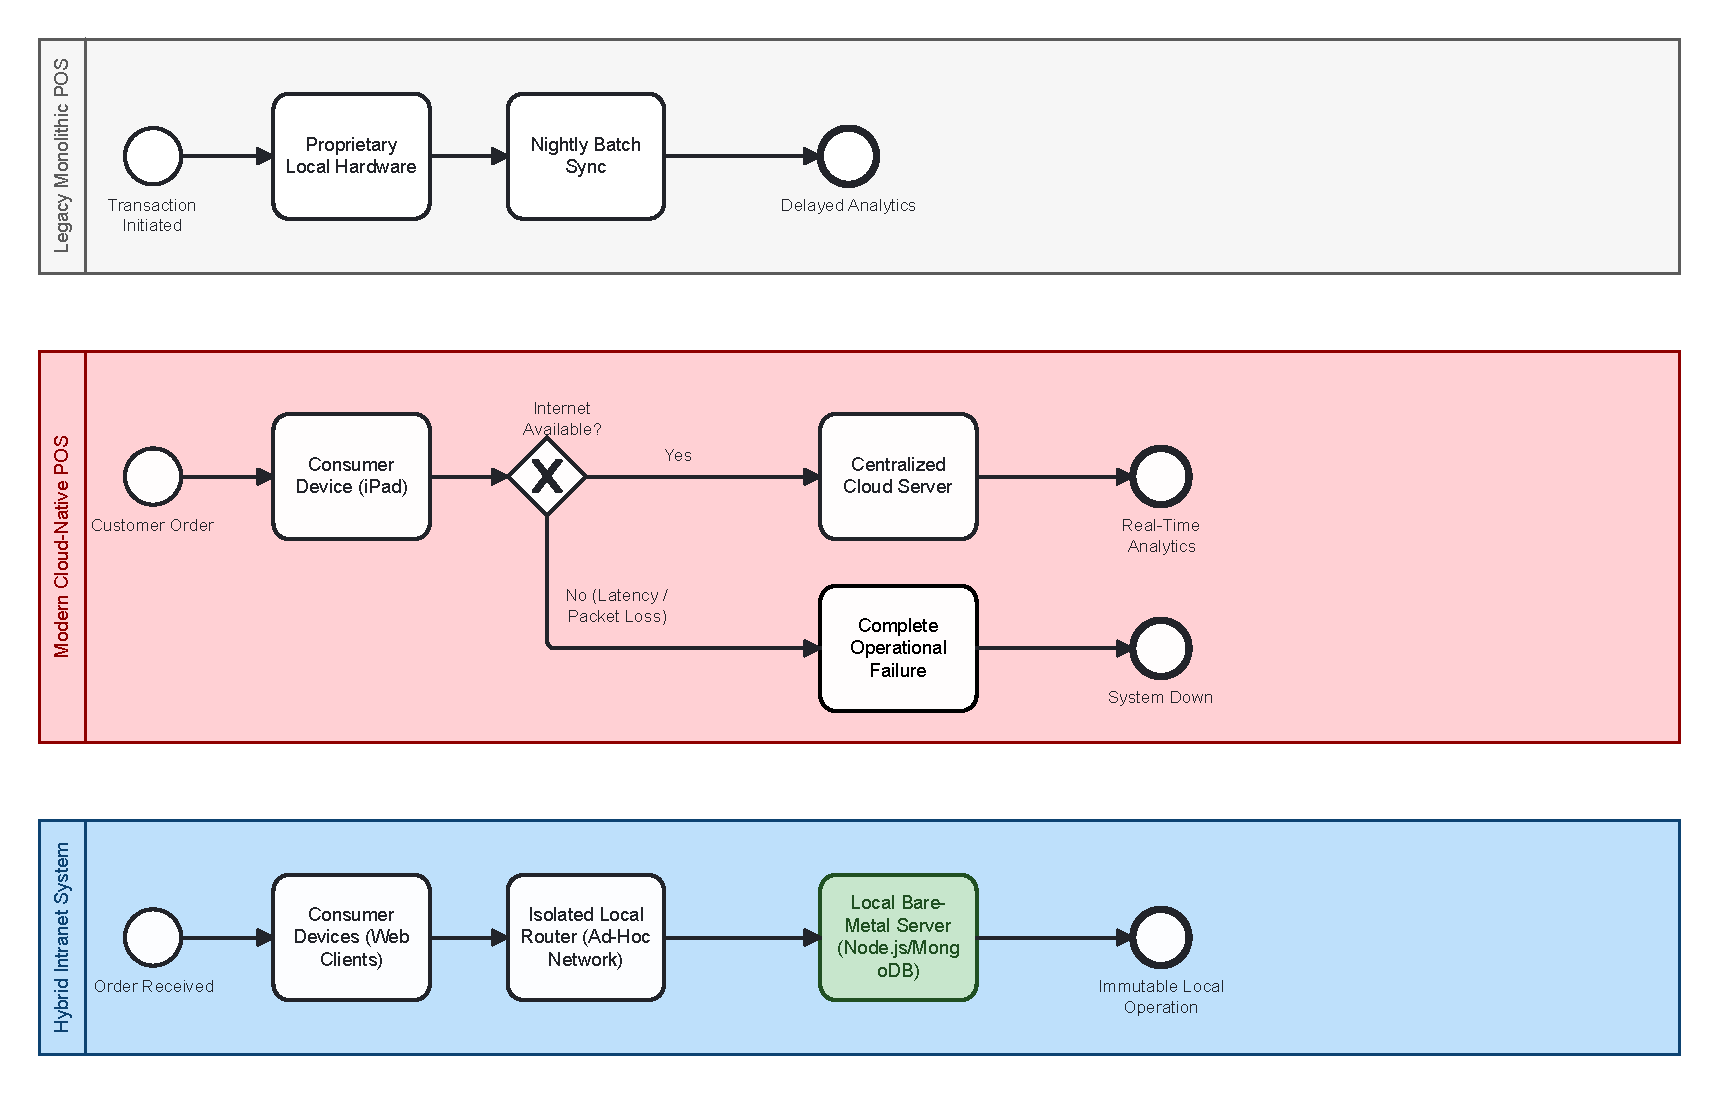
\includegraphics[width=0.9\textwidth]{images/ch1_pos_evolution.pdf}
    \caption{The architectural evolution of Point of Sale systems from mechanical isolation to local-first decentralized networks.}
    \label{fig:pos_evolution}
\end{figure}

\section{Problem Statement: Challenges in Ad-Hoc Networks}

Today, digital order systems are widely used in the food service sector due to the benefits they offer to businesses. However, applying them to temporary environments poses specific challenges due to non-permanent infrastructure, massive customer volumes, low-quality networks, and the need for real-time execution.

\subsection{Common Operational Challenges}
To be both successful and effective in a high-volume process, speed of raw processing is essential. Based on queue theory, as the service rate (the speed at which the items being ordered are served) is significantly less than the arrival rate (the speed at which patrons enter the queue for an item), the service rate is negatively affected as the average service time increases. The smallest delay between transmitting information and receiving it on the network may result in significant issues.

Currently, most systems utilizing traditional web protocols utilize an explicit request/response model. An example of this occurs when an individual requests to purchase a ticket. The request will take hundreds of milliseconds to travel from the ticket-buying tablet located at the cash register via the nearest access network (e.g., mobile cellular network), through the internet backbone, to the cloud server for processing. Once the request has been processed, the response will travel back to the tablet. As previously mentioned, although the time delay stated may appear small and tolerable for most users of the internet at home with a typical computer to complete an e-commerce transaction, this is a large problem when operating in a bar or other high pressure environment.

Although this does not appear to be a problem when the shop is not busy, it is a very bad problem as queues of customers build up and is a direct manifestation of network-induced latency degradation under concurrent load \cite{ibm2019cloud}. As the shopping experience becomes busier, the number of transactions becomes exponentially greater. Another problem encountered by users is when the Point of Sale (POS) interface freezes on a screen and users repeatedly hit the ``confirm payment'' button, thereby inducing race conditions on the server. These race conditions have caused unintended duplicate charges to consumers and catastrophic discrepancies in financial reporting. 

In addition to the previous issue of unintended duplicate charges, data corruption is another, similar, and critical issue that can occur when there are unannounced and temporary network communication problems such as packet loss. For example, when a POS terminal sends a payment confirmation to the central servers of a payment platform. The server processes the transaction, stores it in the database, and then sends an acknowledgement packet back to the POS terminal. Due to heavy local Wi-Fi interference, the acknowledgement packet never reaches the terminal and is lost. 

The server has received and processed the transaction entered, and recorded it in the database. The POS terminal has timed out while waiting for the delayed response packet. The cashier must read the error response at the POS terminal, either re-charge the credit card through logical cashier or ask the customer to pay through another method. In both cases, there will be lost sales, unhappy customers, inefficient operations, possible litigation, or worst case scenario, the cashier may frantically try to keep lines of customers moving by canceling a good electronic transaction just so he can clear an error message. In either case, canceling the transaction will result in incorrect logged inventory and inaccurate daily metrics. 

The previous examples are standard examples used in abstract distributed computing, the so-called ``Two Generals Problem.'' In a computer system, the Two Generals Problem is a theoretical thought experiment that shows the impossibility of perfect synchronization between two autonomous computer systems over an unreliable communications channel \cite{brewer2012cap}. If the communications channel also is unreliable, the computer system cannot detect receipt of packets, unless a reliable hand-shaking protocol is utilized. The above naive design principles and the simple models of eventual consistency that typify many cloud applications are fundamentally inadequate to meet the higher reliability requirements for real-time financial offline accounting in extreme field environments. This profound conceptual communication dilemma is conceptualized in Figure~\ref{fig:two_generals}.

\begin{figure}[htbp]
    \centering
    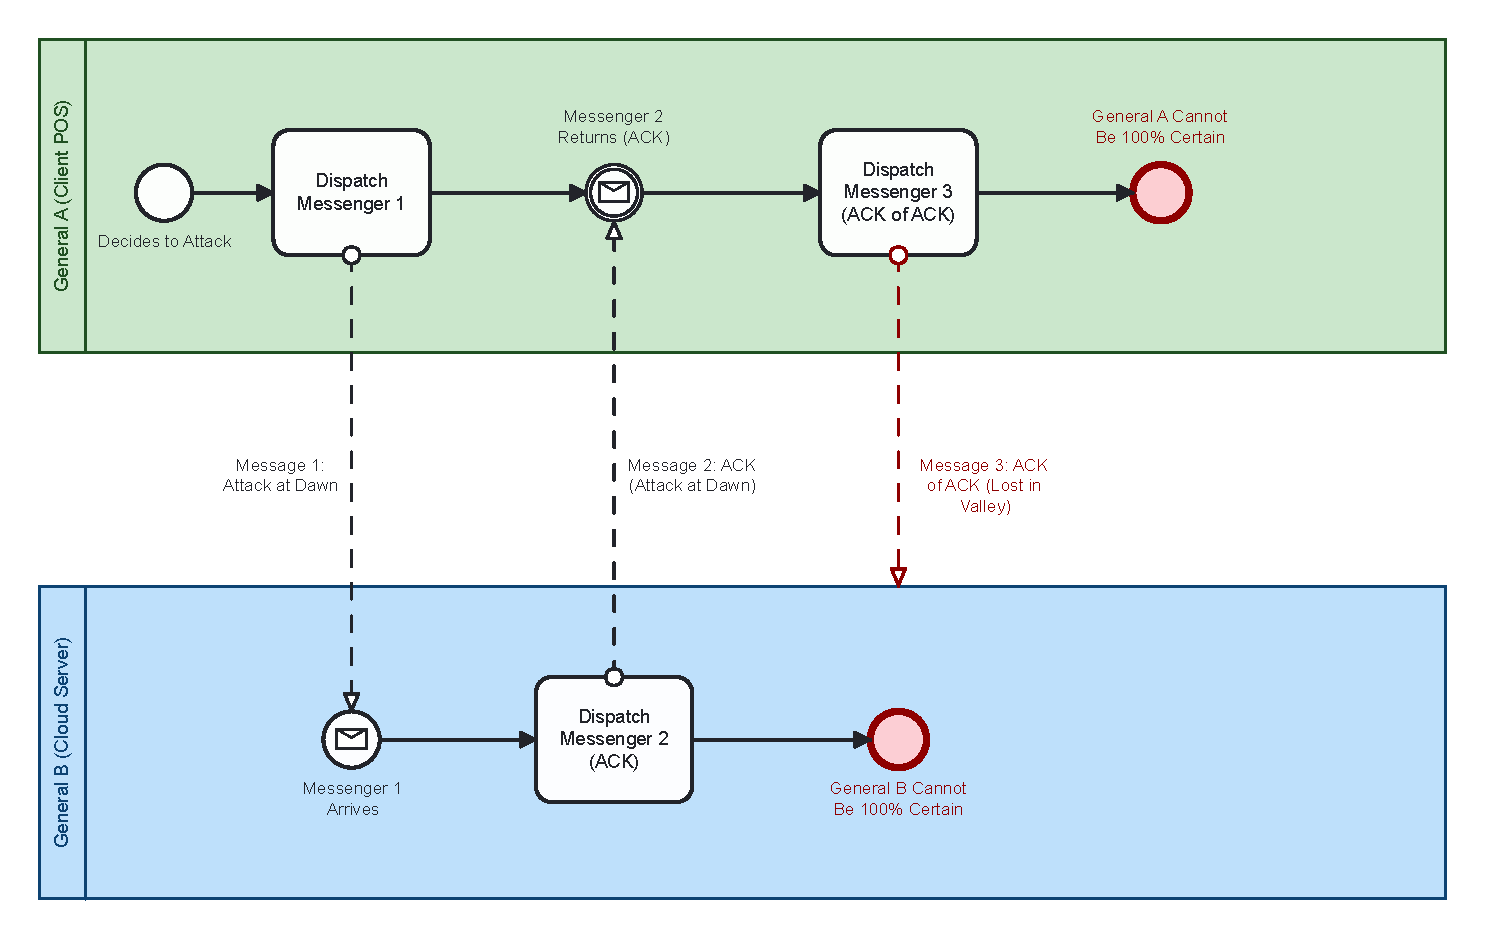
\includegraphics[width=0.8\textwidth]{images/ch1_two_generals.pdf}
    \caption{Visualizing the Two Generals Problem: Achieving deterministic synchronized state over an unreliable ad-hoc network connection.}
    \label{fig:two_generals}
\end{figure}
\section{Research Objectives}

The primary objective of this thesis is the design and implementation of a flexible, user-friendly, and efficient Order Management System (OMS). The specific sub-objectives of the system include: for supporting high transaction loads during temporary events, achieving low network latency, ensuring optimal resource utilization, maintaining high reliability and resilience, minimizing service time for faster customer processing, and effectively managing burst order scenarios.

To address the aforementioned objectives, it is necessary to remove the synchronous request-response paradigm and utilize the highly optimized, persistent, full-duplex communications channels provided by WebSockets \cite{fette2011websocket, mdn2023websocket}.

In addition to the aforementioned, a second major goal of the thesis is to provide strong deterministic guarantees of the absolute consistency of all information contained within every node in the system and to eliminate the extremely deleterious phenomenon of phantom orders. Each node in the system must verify via strict validation on the database side that there exists no state of visual confirmation of the completion of an order by the frontend operator that has occurred until all transactional data has been safely stored and permanently recorded into the persistent ledger on the backend server computer system.

In addition, the design of the system must include the ability to maximize transaction throughput that can be supported concurrently by the system in the most efficient manner possible, while maintaining the highest level of data consistency and eliminating the phantom order issue. Thus, the system must be capable of supporting a minimum of 50 concurrent client devices hammering the system simultaneously, and more than 1,000 complex transactions per hour. Moreover, the system must be able to achieve this level of throughput on a single low-power commodity hardware server (such as an Intel NUC or commodity laptop), to maintain the economic viability of the solution and affordability for individual event organizers who have limited budgets.

Finally, the system is expected to greatly enhance management's operational insights by providing real-time, reactive dashboards as a feedback mechanism. The dashboards will periodically report on sales rates, the current live depletion of each item of inventory, and the performance of individual staff members. Unlike conventional cash registers, which accumulate vast amounts of un-invoiced data dumps in the back office to be reviewed during nightly reconciliation, the system data will be immediately accessible to managers for in-event analysis, enabling them to dynamically allocate staff to busy sections of the venue and suspend the sale of depleted stock items.

\section{Scope and Limitations}

This project focuses on the design and development of a high-throughput order management application tailored for large-scale events, aiming at the efficient entry, processing, and tracking of orders in real-time.

In addition to developing the full software stack of MongoDB, Express.js, React.js and Node.js \cite{banker2011mongodb, express, freeman2019pro, tilkov2010node}, the project will build the deep technical design of the LAN architecture and the strong real-time signal protocol necessary to operate reliably in hostile mission environments. Also, the project will develop multiple modules that support different roles, such as cashier, administrator and kitchen staff, and will implement an advanced algorithmic user authentication system and role-based access controls using a middleware solution on the server-side.

There are a number of large-scale aspects of this project that have been excluded from the scope of the project. Examples of these large-scale aspects include the development of native mobile apps for iOS and Android. Instead of developing native mobile apps for iOS and Android, the project will focus on developing a highly optimized progressive web application (PWA) that can run on most modern standard web browsers \cite{google2020offline}. The choice of PWA technology allows for maximum cross-platform device compatibility with minimal setup/approval requirements from app stores.

However, the project has intentionally avoided the detail low-level engineering of a completely certified, PCI-DSS compliant credit card processing gateway. Lastly, the project assumes that the infrastructure will be built around off-the-shelf consumer tablets and standard IP thermal ticket printers. Therefore, the project will exclude the manufacturing process for creating custom physical hardware.

\section{Thesis Structure}

This portion of the dissertation has been structured in a manner that will allow for a detailed examination of the solution by using a methodical approach. Chapter 2 (Theoretical Background and Technologies) provides the academic base to support the development of the solution based on the models and architectures required to develop high load systems. Chapter 3 (Requirements Analysis and System Design) translates the architectural design as defined by the theoretical components into strict architectural definitions, including an evaluation of the users that will utilize the system, the functional requirements that the system must meet, and the structure of the data. Chapter 4 (Information System Implementation) details the concrete implementation of the backend subsystem, frontend interfaces, and security middleware integration. Chapter 5 (Experimental Evaluation and Empirical Analysis) presents the comprehensive experimental assessment, including comparative baseline studies, stress testing, automated functional verification, and field study analysis. Finally, Chapter 6 (Conclusions and Future Work) summarizes the major technological accomplishments and outlines possible directions for future research and architectural expansion.
\chapter{THEORETICAL BACKGROUND AND TECHNOLOGIES}

\section{Introduction}

Over the last decade, the web has shifted from a static document-centric approach to a dynamic, system based model. Of course, while the main focus of past models were centered around creating content, the real-time web's primary focus has been to synchronize states of clients in real-time. 

Most current web development frameworks depend upon a robust supporting infrastructure, including high bandwidth, and very low latency. 

The implementation of the proposed web application encompasses the development of the frontend, the backend services, and the database. The frontend involves the user interface components designed for high responsiveness. The backend handles the core business logic and event-driven architecture, while the database ensures persistent data storage. Furthermore, the underlying network infrastructure is of particular importance, as it is essential for establishing the reliable and seamless communication required in such demanding environments. 

To address the extreme nature of each scenario, the system was designed to be extremely fast and resilient. This chapter will explain the stacks of software used in building the system through the lens of the theoretical component. This chapter will describe the architecture of the system from the outside-in, beginning with the construction of the front-end, continuing with the back-end mechanisms, how it was deployed, and finally concluding with the security concerns of the system and then provide a historical view of the network.

\section{Web Architecture and Technology Stacks}

The structure as a whole will be based on a custom version of the MERN Stack (MongoDB, Express.js, React, Node.js) \cite{banker2011mongodb, express, freeman2019pro, tilkov2010node} with significant use of WebSockets in order to enable real time features. The reasons behind this selection of technologies are due to their built-in capabilities to perform non-blocking, asynchronous I/O operations which would allow for thousands of users to have simultaneous connections to the application at all times, while never blocking the main thread.

Table \ref{tab:core_tech} outlines an overview of the core technology stack used within each section of the infrastructure.

\begin{table}[htbp]
\centering
\caption{Core Technology Stacks utilized in the architecture}
\label{tab:core_tech}
\begin{tabular}{|l|p{10cm}|}
\hline
\textbf{Domain} & \textbf{Technology and Implementation Role} \\ \hline
Frontend Core & React 18 for component-based rendering and Vite for rapid bundling. \\ \hline
Styling & Tailwind CSS \cite{tailwind} for utility-based styling and executing the custom visual aesthetic. \\ \hline
State Management & Zustand \cite{zustand} for lightweight, decoupled global state management. \\ \hline
Backend Runtime & Node.js and Express.js \cite{express} for the asynchronous event loop and REST routing. \\ \hline
Database & MongoDB for denormalized, partition-tolerant persistent data storage. \\ \hline
Real-time Engine & Socket.io for persistent, full-duplex WebSocket communication between all nodes. \\ \hline
\end{tabular}
\end{table}

\section{Frontend Technologies and Communication Flow}

The new User Interface (UI) for such systems utilizes modern front-end technologies to help alleviate the cognitive load placed on personnel operating in stressful environments, adhering to established user interface design principles \cite{galitz2007}. To achieve this goal in the presentation layer, React 18 was selected to develop the UI as reusable components \cite{react2024docs}. Complementary, Vite was selected over other available solutions, as the development environment, due to its fast hot module replacement and optimized production build generation \cite{vite2024docs}. A utility-first styling system was implemented utilizing Tailwind CSS \cite{tailwind} to create a glassmorphic look with sufficient contrast and legibility while avoiding additional libraries that could slow the initial loading time of the application. Zustand \cite{zustand} was utilized for managing application state (primarily user sessions and authentication). It provides a simple to implement boilerplate to utilize and exposes an API that prevents unnecessary rendering of components subscribed to state changes. Greek and English localization were both supported through utilization of the i18next localization library \cite{i18next2024}. Bilingual staff members may require support for multiple languages in high-pressure operational environments. The most significant aspect of the client-side architecture is the manner in which the client and server communicate with one another. Most web-based applications utilize a ``pull'' communications model to allow for communication between the client and server. However, due to the fast-paced nature of transient event environments (e.g., kitchen's festival operations), the time delay associated with the ``pull'' model is too large for the client to wait for the requested data. To meet the need for a real-time connection, the Socket.io WebSocket protocol was implemented into the system. WebSockets provide a full-duplex, persistent TCP connection between the Node.js back end and the React front end \cite{fette2011websocket}. Once a WebSocket connection is established, the Node.js server and React front end can send data frames to each other with minimal overhead. This provides several advantages, including the ability for the server to push data updates (menus, orders, etc.) to the cashiers' displays without the clients having to request such data, thus reducing network traffic and latency.

\section{Backend Technology Stacks}

The backend system provides continuous access to stored data, has the capacity to handle a large number of users or requests with continued efficiency and reliability, and allows each component to operate independently should all communication be severed between the components' respective servers. A major advantage of this application was its development based on a philosophy of designing the architecture from an architectural standpoint as well as the theoretical perspective of using available memory effectively in high load environments and in synchronizing real-time data across multiple distributed computer systems in a very large computing environment. As such, if one is developing an enterprise-level scalable architecture for such applications, then a robust, fault tolerant architecture would most likely be required.

\subsection{The Concept of an Event}
This event-based architecture indicated the flow of data throughout the system did not occur based on a synchronized request/response sequence for each component that represented an individual part of the systems overall functionality, instead it generated events and reacted to events in the system's operational environment. In this context an event within the operational environment of a system represents a tangible or concrete mathematical operation which causes a change to the systems business logic state. For example, upon confirmation of a purchase (by selecting the ``Confirm Payment'' option) an event payload is generated representing a new order, including the current cart and timestamp. The backend then asynchronously notifies all relevant sub-systems and all active instances of the client at that moment of the change to the state of the system, functioning as a dispatcher. Additionally, decoupling of the functional components of the web application have enabled the creation of reactive dash-boards and notification managers.

\subsection{Node.js and MongoDB}
The back-end of our system was built using Node.js - an open source JavaScript runtime environment. Unlike most application servers, which create a new thread (or threads) per user on the server, Node.js utilizes only one thread and an event loop (reactor pattern). Therefore, while the server waits for an I/O-bound operation, such as inserting an order into the database, it can continue to process the next request of the cashier because it doesn’t block its own thread of execution. It can also insert the order into the database asynchronously (and in the background), and call the appropriate callback once the insert operation has been completed. We chose this architecture because many real-time order management systems are I/O-bound instead of CPU-bound. By utilizing a Node.js server, we can eliminate the need to create and maintain thousands of threads and can therefore provide a high quantity of concurrent web-socket connections - especially useful in environments with limited hardware, such as festival deployments.

For persistence of our data, we utilized MongoDB. Theoretically, the choice of a database for distributed systems is largely based upon the CAP theorem, which states that a data store can only provide two out of three of the following properties: consistency, availability, and partition-tolerance \cite{brewer2012cap}. Relational databases typically focus on maximizing consistency, so if the network goes down, they will lock writes to prevent divergent data. Because we have chosen to prioritize availability and partition-tolerance in our deployment, we decided to utilize MongoDB with configuration options to maximize availability. Additionally, we employed a denormalized document model. Instead of utilizing expensive relational joins to pull together all of the relevant details of an order from the database, we included all of the details of the order within a single document.

\section{Network Infrastructure}

The physical requirements for the use of our application necessitate that we take a ``local first'' approach to installing the application as opposed to other cloud-based applications. For instance, during festivals, there generally is no reliable Internet access available to users who are not located inside the festival grounds. In order to alleviate this problem, we have designed our application to be a self-contained application that is able to function locally without the need for an Internet connection. To make this feasible, we are utilizing the full MERN technology stack to deploy all of the necessary server infrastructure to dedicated servers in the area where the festival is being held. We will also utilize a local area network (intranet) to connect all of the tablet devices utilized by cashiers and cooks. We will accomplish this using a combination of both consumer-grade and enterprise-grade routers to create a dedicated local Wi-Fi network. This will enable us to eliminate the need for data to be routed over a mobile tower or the general public Internet backbone. Due to the fact that this local network will include the complete transactional flow of the application, it will be capable of avoiding any potential delays or latency that would result from the use of a cloud-based solution. As a further measure of redundancy, if we have very limited bandwidth over the Internet, we will utilize the secondary backup systems to periodically sync up with the primary systems.

\section{Application Security}

The security needs of the application architecture were taken into account as it was developed. Zero trust architecture was used for all web socket messages and all api calls made by the application are authenticating. The jwt stateless authentication approach has been used to achieve the goal of partition tolerance and to decrease the amount of session queries to the database. The server creates an access token with the user's information and the server creates an access token with the user's details and a digital signature when the user logs onto the site. Each subsequent request contains the token created when the user logged onto the site, and the token is stored on the user's computer, allowing the server to use a mathematical validation to determine if the token is valid or invalid, rather than the need to have the server verify the status of the token in a data storage system. The server is thereby relieved of additional workloads associated with verification, and provides the assurance that a user remains authenticated even if the server is unavailable as a result of planned server maintenance or unplanned server hardware failure.

\section{Comparative Analysis of Technology Stacks under High-Load}

To confirm that the MERN stack and the design decisions made with respect to architecture are theoretically correct, we will analyze how the behavior of web development stacks changes when under extremely high loads and also when there is extreme instability in the local area network (LAN) communications. The scenario to be used for this analysis is one where hundreds of users are attempting to synchronize all of their transactional data at the exact same moment.

In a traditional LAMP-based setup (Linux, Apache, MySQL, PHP), a new process is spawned for every PHP session. For each user's request, a completely new instance of the PHP interpreter is brought into memory. This results in the server having to use a great deal of RAM. Since servers only have a limited amount of RAM, this eventually leads to ``thrashing.'' Thrashing occurs when the operating system spends the majority of its time moving data out of memory to disk and vice versa. This renders the machine unusable.

Most large-scale business applications utilize the Java Spring framework which utilizes a thread-per-connection model. While threads consume significantly less memory than spawning processes, when you have many simultaneous connections (e.g. thousands of simultaneous connections) the CPU is spending the vast majority of its time switching contexts as opposed to actually executing the program. Therefore, threads do not provide a suitable solution for extremely high levels of I/O concurrency. In contrast, the MERN stack utilizes an asynchronous event loop, allowing the majority of the requests coming from the client to be processed by a single thread. As such, the MERN stack requires substantially less memory per connection, and does not incur the significant CPU overhead associated with the context switching of threads.

\section{The Evolution of Point of Sale (POS) Architectures and Related Work}

A description of the overall objective of the developed system requires a historical overview of transaction processing. In many ways, the evolution of POS technology has been driven by advancements in both connectivity and data accessibility. The first generation of POS systems (which existed from approximately 1970 through 1999) were essentially electronic cash registers. These systems were primarily stand-alone hardware devices that offered extremely high levels of reliability, however, they were essentially separate data islands that did not offer any real-time operational intelligence. The second generation of POS systems involved the introduction of client-server systems utilizing local area networks (LAN). While client-server architecture allowed for the centralization of data, creating LANs for temporary events proved to be logistically cumbersome, and the potential for introducing single points of failure became a significant issue. Cloud-based, native software currently represents the standard in the POS industry. With the exception of local maintenance issues, this model creates a serious problem in unstable environments. When the external network experiences problems, these systems ``freeze,'' thereby failing to meet one of the fundamental requirements of service availability. The emerging architecture models (one example being the model utilized in this thesis), which combine modern web technologies for both the interface and the logic, while deploying the server locally, provide a new generation of POS solutions. The hybrid approach enables the same advantages of rapid development using web frameworks as the application's logic and user interface are executed locally. 

Although there is an abundance of literature related to POS systems, the majority of the research is focused on either the use of analytics in retail environments or the enforcement of security regulations in a corporate environment. Additionally, although there have been numerous studies regarding the use of offline-first web architectures, the majority of the research lacks examples of how these architectures can be applied in a real-world scenario, especially when dealing with multi-user applications that require real-time synchronization in highly latencies conditions. The primary void within the existing body of knowledge and practical applications is the lack of a system that addresses the latency problem and utilizes modern, component-based web frameworks, along with an event-driven, local-first topology specifically designed to operate effectively despite the limitations presented by temporary, large-scale events. This thesis fills this void by providing a detailed description of a system that directly addresses this issue through the implementation and field-testing of the described architecture.
\chapter{REQUIREMENTS ANALYSIS AND SYSTEM DESIGN}

\section{Introduction}

The Systems Development Life Cycle explicitly outlines that the Requirements Analysis Phase is the foundation upon which all successful software projects are built. As such, given both the complexity and risks present within a large event environment, this phase becomes even more critical. The failure to identify and document specific ``edge cases'' (i.e., loss of communication with a payment terminal during the middle of a transaction, or two wait staff making modifications to the same ticket) may result in potential financial discrepancies or disruptions.

Compared to corporate settings, where the collection of requirements occurs via multiple, structured interviews conducted over a long term, the event environment has a much different dynamic. The system will serve two purposes: it will act as a hard, non-elastic ledger system for the event organizer's financial needs, and it will be utilized as a soft, flexible interface for use by untrained temporary employees. This chapter will detail the conversion of problem statements into specific architectural specifications.

\section{Development Methodology}

The development of the localized OMS in environments characterized by instability or ``hostile'' network conditions requires flexible and iterative methodologies. The complexity and variability of such networks make traditional linear models, such as Waterfall, unsuitable, as they do not support rapid adjustments to the system's design or architecture. An Agile/Scrum methodology has been selected as the methodology to direct the OMS Software Development Life Cycle \cite{scrum2020guide}, an incremental approach to software development and Agile methodologies. In Agile, the iterative process breaks down the large engineering problem into smaller chunks of the total effort. At the end of each sprint (a short, time-boxed period during which specific work is completed), a predefined quantity of new functionality is implemented, tested, and prepared for release to production. This allows for incremental releases versus creating a detailed master plan upfront that may become obsolete after the first deployment. There are typically three main roles in Agile: the Product Owner (responsible for maintaining the Product Backlog and defining what the next release includes), the Scrum Master (responsible for the Scrum process and removing obstacles), and the Development Team (team members responsible for all disciplines needed to create the product). The development was performed through multiple two-week sprints. The sprint planning session occurs at the start of each sprint to define short term engineering objectives and select items from the Product Backlog to work on during the current sprint. After these objectives were identified, daily stand-up meetings occur so that members of the development team can discuss their status and issues relating to the technical aspects of the project. Two types of review sessions are held at the conclusion of each sprint: a sprint review meeting to demonstrate the results of the work completed during the previous sprint, and a sprint retrospective meeting to assess the process of completing that work. Both sessions provide an opportunity for iterative improvement of the system being built, but especially for improving the resilience of the system one component at a time. Figure~\ref{fig:agile_scrum} illustrates how the Scrum model can be properly utilized when developing software.

\begin{figure}[htbp]
    \centering
    % TODO: Create a diagram showing the Agile Scrum lifecycle (Sprint Planning -> Daily Scrum -> Sprint Review -> Retrospective)
    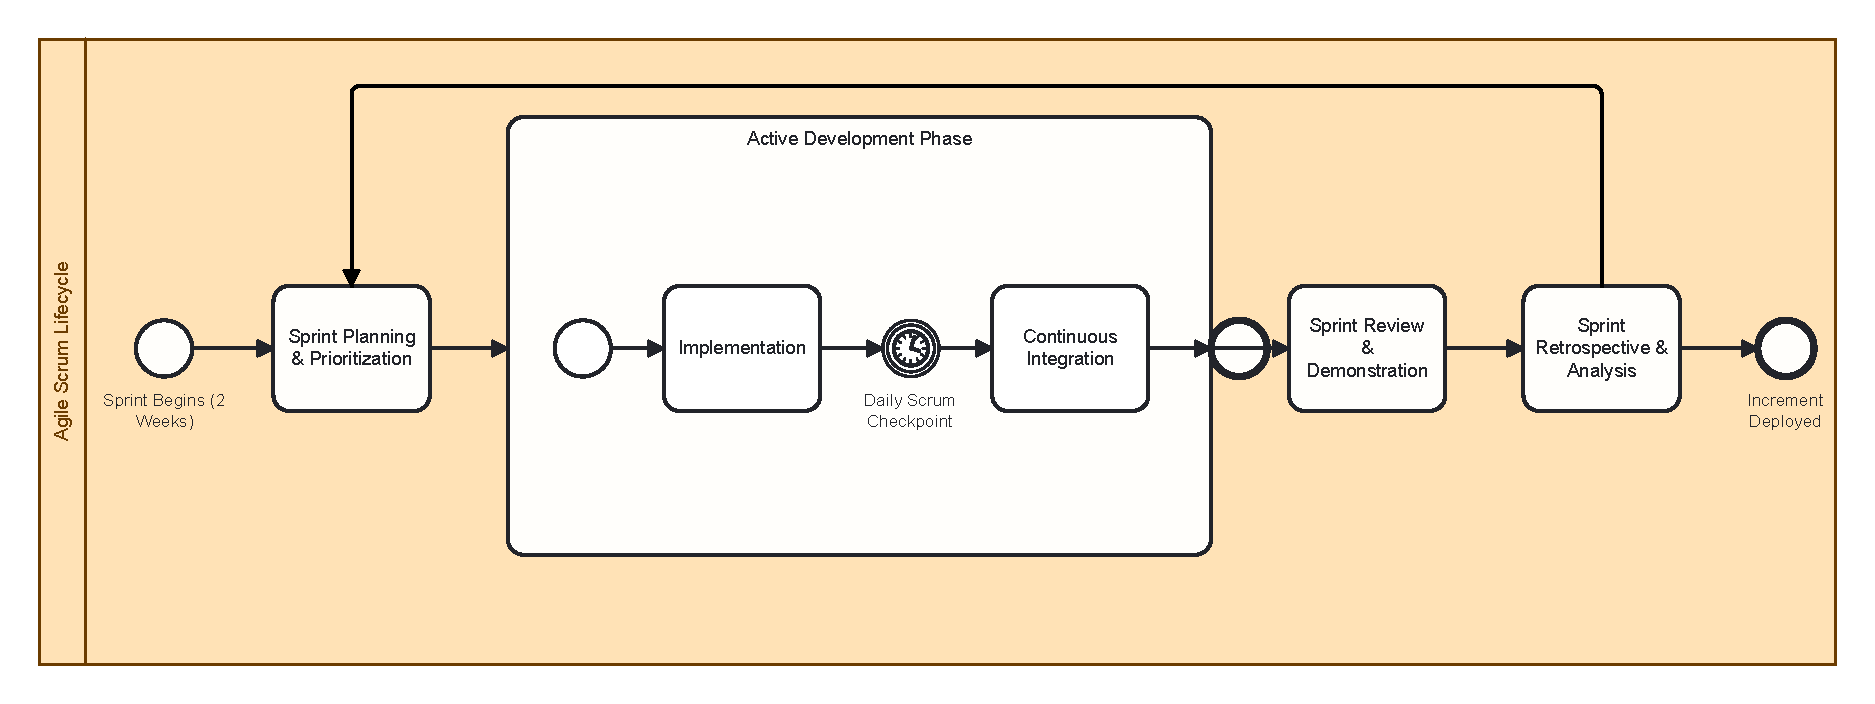
\includegraphics[width=0.8\textwidth]{images/ch3_agile_scrum.pdf}
    \caption{The iterative Agile Scrum methodology driving the continuous delivery of the developed architecture.}
    \label{fig:agile_scrum}
\end{figure}

Using this model, we had our first software development cycle to create the minimum viable core transaction loop. The first important sprint toward achieving this specific objective was to set up the base components of the hierarchical product catalog, cart logic, and RESTful order submission API. The second sprint was dedicated to building the real-time communication layer required to support both sides of the interaction. The architecture was formally documented using WebSockets instead of polling requests to enable the kitchen interface to receive updates regarding orders and to support bi-directional communication without user interaction. Finally, the last few sprints were directed toward hardening of the system and implementation of protection against edge cases that arose while running in the adversarial environment of a retail store.

\section{Stakeholder Analysis and User Personas}

In order to ensure that the deployment of the system actually fulfills all the requirements of its end-users' operational environments, we created user personas. Theoretical representations of users. These theoretical representations of users guided the design of the interfaces and the prioritization of system functions throughout the lifecycle of the project.

To guarantee that the architecture of the system will meet the performance expectations of high-volume event services, three individual user personas were created to guide the architecture. Each user persona will interact with a custom-built module within the system, designed to accommodate their own workflow and expected system behavior.

The first group, called ``cashiers,'' will sit directly in front of the line where customers physically wait. Their sole access to the system will be through an interface for entering orders and confirming payments. Because cashiers have very limited time during peak hours, the Cashier's Module has been built around maximizing speed. This has led to the use of large, high-contrast buttons (touch targets) that are organized by product category. The key expectation of this user is that there is a frictionless experience immediately when accessing the system, which will never block or freeze due to fluctuations in the network. If there is some type of transaction error condition, the system should immediately display a clearly defined degradation path from the point of error rather than a seemingly endless ``loading'' animation.

The second group includes cooks and baristas working in a production environment. While each persona interacts with the system in different ways, both are primarily information consumers who react to an incoming stream of data. The Kitchen module serves as a real-time electronic ticketing system. Cooks do not need to enter complex information, instead, they confirm whether a ticket is open and then indicate it is complete with one single tap. In order to fulfill this persona, the architecture must provide 100\% guaranteed data integrity -- a ticket can never be removed from their view until they manually complete it, and delayed tickets entered offline by cashiers must always correctly integrate into the current queue upon re-establishment of network connection.

Finally, administrators require a real-time dashboard providing a complete view of all aspects of operations. Typically located in a back-office setting, or via a mobile device while moving about, they monitor in real-time such things as current sales velocity, what products are quickly being depleted, and which cashier nodes may have issues connecting to the network. Because of this need for continuous dynamic updates to visualizations, the Administrator module heavily depends on reactive capabilities provided by an event-driven architecture in order to update visualizations dynamically without the administrator needing to continuously manually reload web pages.


\begin{figure}[htbp]
    \centering
    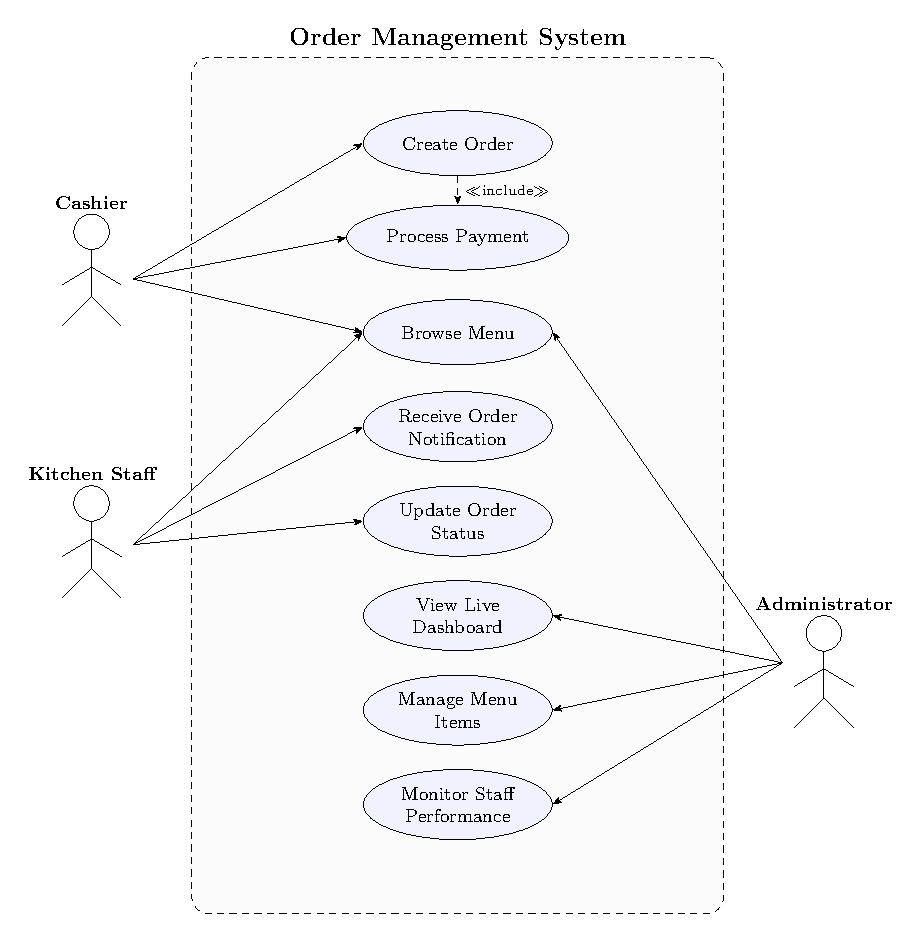
\includegraphics[width=0.85\textwidth]{images/ch3_usecase_diagram.pdf}
    \caption{UML Use Case Diagram illustrating the primary interactions between the three identified user personas and the core system functionalities.}
    \label{fig:usecase_diagram}
\end{figure}

\section{Functional Requirements}

To meet the various operational needs of the chosen environment, the system was created with a number of important functional requirements. The design of the architecture must allow for multi-channel order entry. This means the system will be able to generate and instantaneously send orders through different business areas (e.g., cash registers, kitchen, etc.). Additionally, the system will have to allow for dynamic product customization in order to accommodate multiple levels of products. This would enable a cashier to make adjustments to product ingredients or add comments on the fly when creating an order.

The first step after an order has been entered into the system, is that it will need to automatically route sub-sets of the order based on intelligent logic to direct them to the right area(s) where they can be prepared. For example, if you are preparing food at a restaurant kitchen, the items that go into preparation should only show up on your screen. There also must be some type of real-time life cycle management to track all transactions continuously and reflect all states of change from pending to handing off the last item. Lastly, one of the most important elements is high throughput, this means the capability to process an extremely large volume of orders per minute while maintaining adequate capacity and never losing or degrading the data.

\subsection{System Workflow Description}

To begin, system processes are built to model the main business functions of each persona. At a very high level, the workflow begins at checkout, where the cashier creates a new order at the point-of-sale. The cashier will then select products from the product catalog displayed at the point-of-sale. When the products have been added to the shopping cart and the total has been entered, the cashier will click ``checkout,'' proceed to payment, and the system will perform a ``handshake'' with an external payment terminal. Upon receiving a positive encrypted response from the banking gateway, the system will create a new sequential human-readable order number, record the confirmed order into an immutable MongoDB data store, and broadcast an order event via WebSockets to each of the waiting kitchen tablets so the kitchen will know to prepare the new order. Special cases are also handled. For example, if an order for the last item in stock by the cashier, prior to having time for the local terminal to confirm payment, the system will check whether stock is sufficient. If the stock is insufficient, the order will be denied, the item will not be sold, and the cashier will be asked to replace it or find another method of selling the item. These business processes were modeled using BPMN, as described above, and formally presented in Figure~\ref{fig:bpmn_order_flow}.

\begin{figure}[htbp]
    \centering
    % TODO: Ensure the BPMN diagram (from bpmn.io) for the Order Creation Flow is placed here
    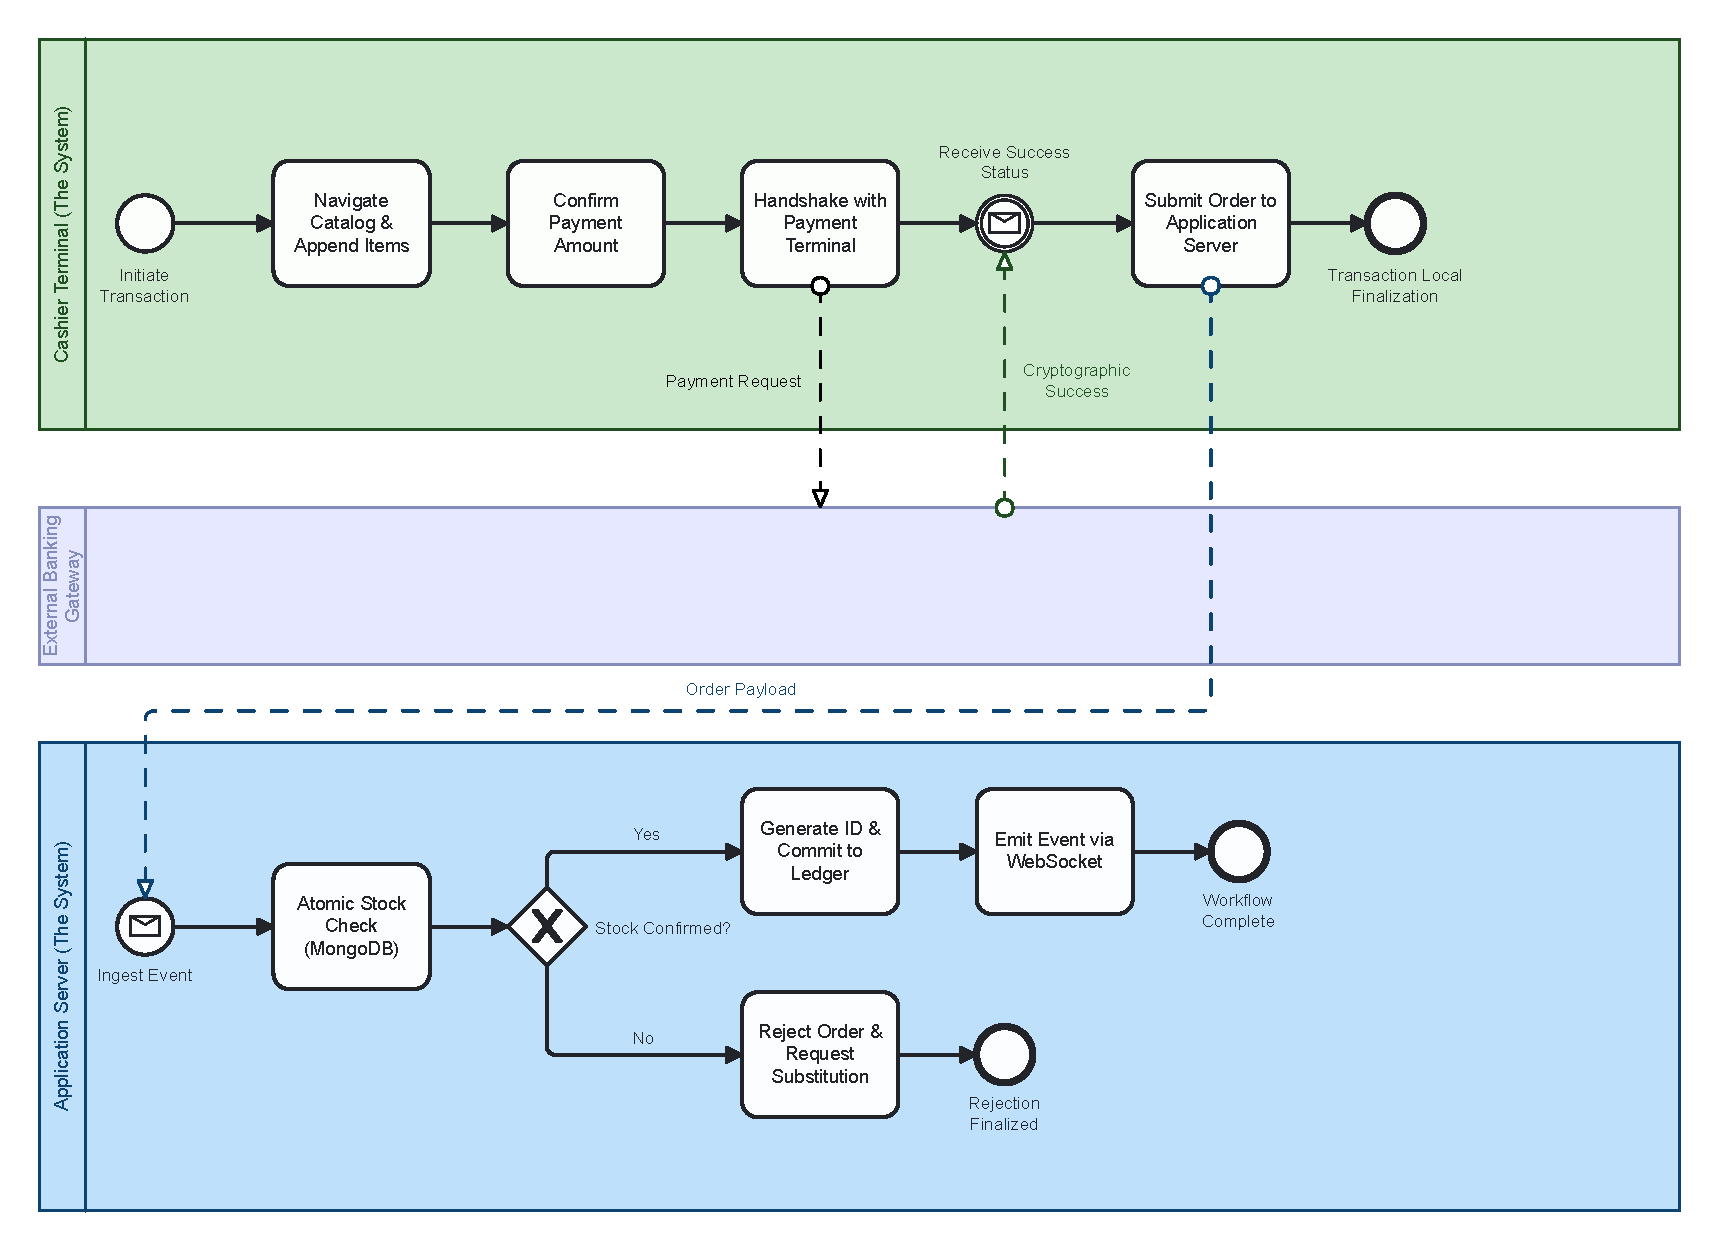
\includegraphics[width=0.9\textwidth]{images/ch3_bpmn_order.pdf}
    \caption{BPMN Model depicting the logical flow of Order Creation, from cashier input to database persistence.}
    \label{fig:bpmn_order_flow}
\end{figure}

The kitchen interface represents a separate workflow from those processed by the cashier. In the kitchen, the interface receives instantaneously a notification of each new confirmed order, displays any special preparation notes, and sounds an audible alert to notify workers when a new order is entered. Using macro-gestural inputs, the chef goes through each process state of their work from pending state to completion state. This allows us to represent the different process states of the chef in the BPMN diagrams shown in Figure~\ref{fig:bpmn_kitchen_flow}.

\begin{figure}[htbp]
    \centering
    % TODO: Ensure the BPMN diagram (from bpmn.io) for the Kitchen Display Flow is placed here
    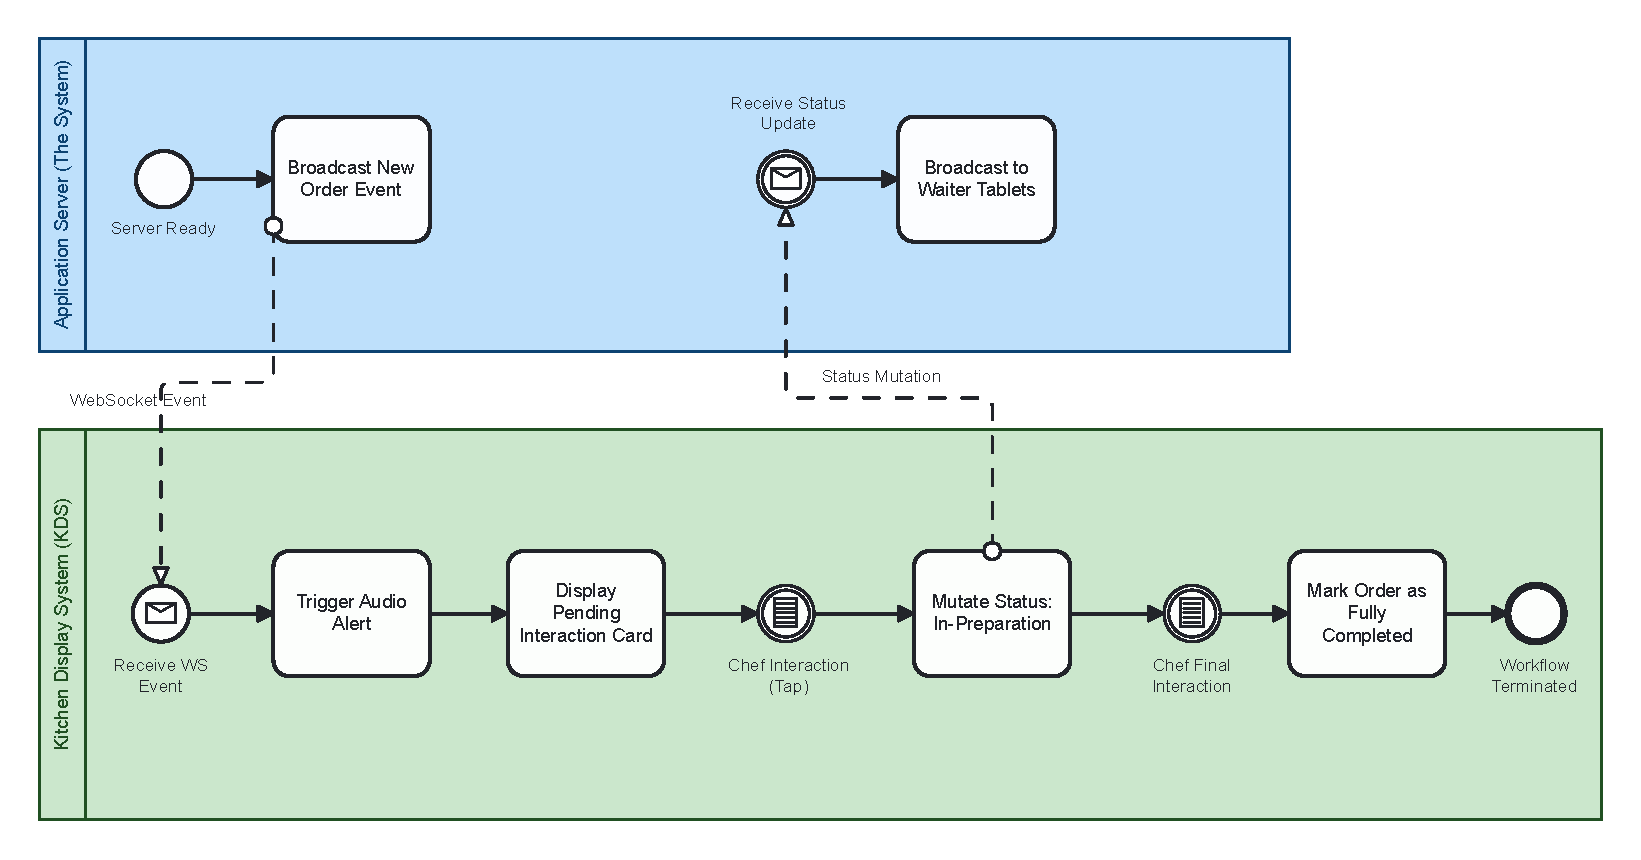
\includegraphics[width=0.8\textwidth]{images/ch3_bpmn_kitchen.pdf}
    \caption{BPMN Model depicting the Kitchen Display workflow, detailing real-time event reception and order fulfillment.}
    \label{fig:bpmn_kitchen_flow}
\end{figure}

For kitchen order management, the client application running on the kitchen tablet and the Node.js server must be in the same secure WebSocket room. When a confirmed order notification is sent from the Node.js server, the kitchen tablet receives an audible sound alert and a card for the order is added to the pending column of the user interface with corresponding animation. Once the user has selected a card to be prepared, the UI will indicate that the card is being prepared and the server will send a server push message to all waiter tablets that the card is being prepared. This completes the loop between service staff and the kitchen.

Inventory levels should be maintained based on ingredient requirements rather than goods available for final sale. For example, in regards to a burger, there are only three ingredients needed: buns, patties, cheese. Therefore, when a customer purchases a burger, you need to decrement each ingredient one at a time. The additional challenge here is if any key ingredient reaches zero, the availability of all products is immediately removed from all point-of-sale terminals. During initial play testing, it was discovered that failing to account for all components while completing a transaction would cause discrepancies in inventory count.

\section{Non-Functional Requirements}

Functional requirements explain what this System will do. Non-functional requirements represent how well this System will function when subjected to extreme operating conditions. All the restrictions are compared to current architectures \cite{iso25010}. 

Performance: The key path (the amount of time to confirm a payment and then send the confirmation message to the kitchen display) will require near-instantaneous execution without noticeable delay. Resource utilization: The Core Server Process will not consume more resources than the average commodity hardware has available (cpu, memory, disk space), and can support up to 100 concurrent clients, of which up to 50 may maintain persistent WebSocket connections simultaneously. The infrastructure must also maintain a minimum of 60 frames per second throughout the entire UI.

To force the restarting of the local servers, the reliability requirements dictate that all Active Clients will be able to connect to the local server again within 5 seconds. To avoid the ``thundering herd'' problem (all active clients connecting to the local server simultaneously) an exponential back-off algorithm is utilized. 

The system must implement database journaling and strict write concerns to ensure that financial information remains valid even if there is a loss of power immediately following an operation having been completed. Learnability is also defined as a critical non-functional requirement. For example, the system must enable a temporary employee to successfully complete a transaction independently within 5 minutes of initial use. In addition to error prevention, secondary manager authorization is also utilized for destructive operations (i.e., delete logged orders, cash refunds, etc.) to prevent accidental or malicious actions by someone utilizing the system. 

The stateless security policies that restrict a physical waiter's ability to create something via an API call (all API calls will contain a JSON Web Token and role based permissions will be applied on the first router level) will prohibit a waiter from making a request to change a product's price \cite{ferraiolo1992rbac}.

\section{Data Modeling and Schema Design}

The success of a Node.js-based API depends largely upon the efficiency of its underlying data structures. When functioning in a high volume transactional environment, an improperly structured relational query quickly becomes a system bottleneck.

For our Order Management System (OMS), we use a NoSQL approach using MongoDB \cite{banker2011mongodb} where we prioritized read/write speeds over heavy normalization. We use a somewhat denormalized document structure. In our system, for instance, we don't just insert the itemId into an order line and force the database to pull off an expensive JOIN every single request in order to get the price and name of the item - we embed the fundamental qualities of the item into the Order document at the exact time of the initial retail transaction. In doing so, we essentially lock the orders to exactly what they were at the time of purchase in the event the actual menu item is later configured to a different price. It also extensively lowers the computational cost associated with searching large order histories.

\begin{table}[htbp]
\centering
\caption{Primary Database Schema Structures for Orders and Menu Items}
\label{tab:schemas}
\begin{tabular}{@{}lll@{}}
\toprule
\textbf{Collection} & \textbf{Key Fields} & \textbf{Data Type / Relation} \\ \midrule
\texttt{Order} & \texttt{orderNumber} & String (Unique) \\
 & \texttt{status} & Enum (pending, preparing, ready, etc.) \\
 & \texttt{items} & Array of \texttt{orderItemSchema} \\
 & \texttt{totalAmount} & Number \\
 & \texttt{paymentMethod} & Enum (cash, card, iris, etc.) \\ \midrule
\texttt{MenuItem} & \texttt{name} & String \\
 & \texttt{price} & Number \\
 & \texttt{category} & ObjectId ref: \texttt{Category} \\
 & \texttt{available} & Boolean \\
 & \texttt{stock} & Number \\ \bottomrule
\end{tabular}
\end{table}

Table~\ref{tab:schemas} outlines the primary transactional schema structures utilized in the database. The complete database schema also encompasses supplementary entities, including Users (for role-based access control), Categories, and Ingredients, which are essential for full system operation.

\section{System Architecture and Component Interaction}

The architecture of our Order Management System (OMS) follows a strict decoupling between the client and server. The client, a Single Page Application (SPA), created with React, oversees all elements of the application's user interface, including user routing and the presentation of information. Our Node.js and Express RESTful API acts as our service tier, taking business logic, database queries and security, and completely separates it from the user interface.

To facilitate communication between the React frontend and the Node.js backend, a unified gateway layer built on Axios \cite{axios} was developed. To ensure security, all asynchronous requests from the client include a JSON Web Token (JWT) in the HTTP Authentication Header, which serves as a stateless handshake, cryptographically authenticating the user’s identity and specific roles without requiring the server to look up the session state in the database. Because it is completely separated from the database and session server, the backend API can be scaled independently, or replaced completely by a different language stack without requiring significant modification to the client codebase.

\section{Real-Time Communication Protocols}

The need for real-time data processing in an Order Management System (OMS) performs far better than HTTP polling, an HTTP polling use case for this example would include the client sending many requests to the server requesting new tickets to send. At high volumes, HTTP polling will have both latency and network overhead. To improve both latency and network overhead, we utilize real-time, bidirectional communication (WebSockets) by adding the Socket.io library. This establishes a bidirectional communication pipeline between all clients and servers. All non-real-time related functionality (such as static configuration data), that do not require communication via WebSockets (for example REST APIs) are utilized. Once authenticated on the socket connection, the clients subscribe to multiple ``communication rooms'' based upon their role and current service usage (for example, a cook subscribes to the `kitchen` room) \cite{socketio2024rooms}. When the API processes an order, it emits an `orderCreated` Socket.IO event into the `kitchen` Socket.IO room that the React frontend has subscribed to. The React frontend then updates its Zustand state tree in memory and triggers a full page update with the latest ticket information. This entire process takes place within milliseconds and is vastly superior to a polling-based solution.

\begin{table}[h]
\centering
\caption{WebSocket Event Specification}
\label{tab:websocket}
\begin{tabular}{|l|p{3.5cm}|p{6.5cm}|}
\hline
Event Identifier & Target Room & Operational Result \\ \hline
\texttt{new-order} & kitchen\_staff & Delivers the full order object and triggers the audio alert. \\ \hline
\texttt{order-status} & service\_staff & Updates the visual pickup board with the prepared item. \\ \hline
\texttt{scarcity-alert} & cashier\_terminals & Forces the immediate disablement of out-of-stock product buttons. \\ \hline
\end{tabular}
\end{table}

\section{Application Programming Interface (API) Specification}

A powerful RESTful API will be required to call the CRUD (Create, Read, Update, Delete) methods for system configuration and historical data as well as implement the complex first-order business logic and validation. The API adheres to the REST standards and RESTful API guidelines. All API endpoints utilize the standard HTTP verbs (GET, POST, PUT, DELETE) to communicate with logical resources. In addition to that, all API endpoints have the prefix \texttt{/api/v1/}, making it easy to perform future versions without breaking existing clients. By isolating this complex validation logic in these API controllers, we keep the database organized and uncluttered, while keeping our WebSocket layer very lightweight and only responsible for fast messaging.

\begin{table}[h]
\centering
\caption{REST API Interface Specification}
\label{tab:rest_api}
\begin{tabular}{|l|p{3cm}|p{2cm}|p{6cm}|}
\hline
Method & Endpoint & Access & Description \\ \hline
POST & /api/auth/login & Public & Authenticates user credentials and issues a secure JWT. \\ \hline
GET & /api/products & All Roles & Fetches the complete product catalog for local caching. \\ \hline
POST & /api/orders & Cashier & Creates a new order entry and fires internal socket triggers. \\ \hline
PUT & /api/orders/:id & Kitchen & Updates a specific order's status (e.g., from pending to ready). \\ \hline
GET & /api/reports & Admin & Generates comprehensive financial aggregations for dashboards. \\ \hline
\end{tabular}
\end{table}

\section{Security Architecture and Access Control}

A comprehensive approach to security is taken because of the possibility of the server being exposed to an insecure Local Area Network (LAN), thus the use of a Zero Trust Architecture Design Strategy is employed. All incoming requests to the server are viewed as potentially malicious, regardless of their origin within the LAN. When a user logs in, the server generates a JSON Web Token (JWT) that verifies user credentials \cite{ferraiolo1992rbac}. Following login, the server creates a cryptographically generated token, using the user's unique ID and role, which is then passed to the client, who stores it locally. Although the server retains no session data, any subsequent requests made to the server require a valid signature to exist on the original token. A stateless system is critical for building a fault-tolerant system. If the Node server fails and restarts while an event is occurring, it will lose ``active sessions'' since everything relies on cryptographic authentication, not on the state of the server.

Using middleware that utilizes Role-Based Access Control (RBAC), access to resources is controlled prior to the application logic processing the request (i.e., deleting a menu item). The RBAC middleware checks the JWT to see if the roles included in the JWT (i.e., admin) contain sufficient privileges to allow access to the requested resource. If it finds insufficient privilege, it returns a ``403 Forbidden'' HTTP status code and rejects the request. This prevents unauthorized modifications of stateful data at the outermost API boundary. Security logic should always be separated from application logic, never mixed together.

\begin{figure}[htbp]
    \centering
    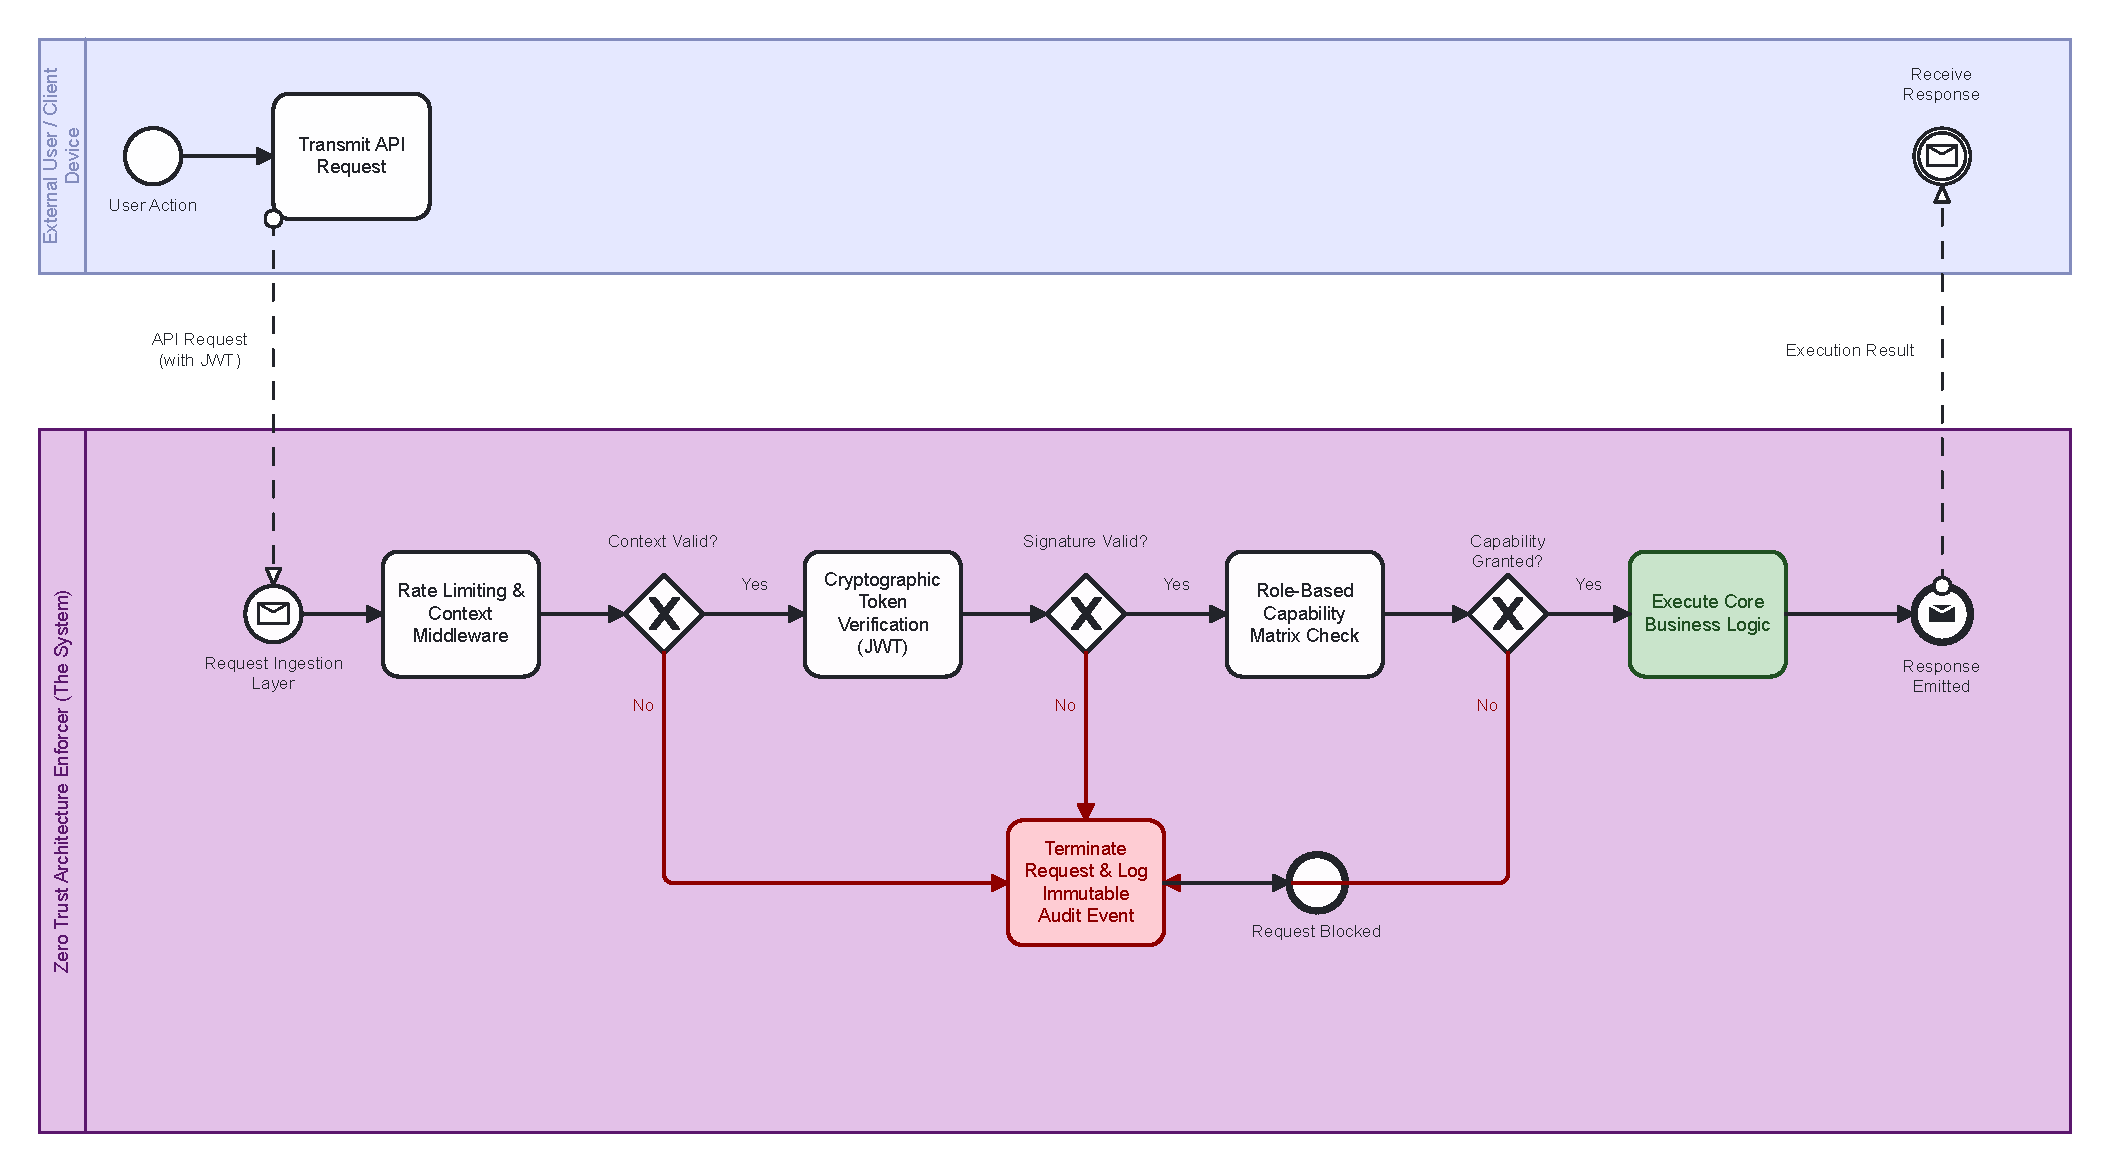
\includegraphics[width=0.9\textwidth]{images/ch3_zta_diagram.pdf}
    \caption{The Zero Trust Architecture of the system, enforcing strict capability-based authorization at every interaction layer.}
    \label{fig:zta_architecture}
\end{figure}

Additionally, a full threat modeling analysis was performed several times during the development lifecycle. Threat modeling tools from industry-standard sources were utilized to help identify and classify threats. One example of these tools is STRIDE. The word STRIDE represents Spoofing, Tampering, Repudiation, Information Disclosure, Denial of Service, and Elevation of Privilege.

Impersonation or identity theft or masquerading is referred to as spoofing. Through the utilization of cryptographically generated JSON Web Tokens (JWTs) with short expiration dates and validating signatures at each API endpoint, the risk of spoofs is greatly reduced. Because of these methods, even if an intercepted JWT is obtained in transit it is essentially worthless because it would expire almost immediately due to its expiration date.

An attacker may try to modify the product price somewhere in the checkout path, either before sending it to the customer or after receiving it from the customer while traveling to the payment gateway. The solution described here protects against this type of attack by way of an absolute validation process. Rather than relying solely on the total price value sent from the client UI to the backend API, the backend API uses a database-based pricing model as the sole trusted source.

In an extreme case, a dishonest entity could deny performing an action although there exists proof that it occurred (a cashier takes physical money from a customer but later claims ignorance regarding how an item was removed from inventory). These types of risks can be completely mitigated by establishing an immutable, append-only database that records each logical operation, including the cashier ID and timestamp of each operation.

Information disclosure occurs when any sensitive information stored in internal data (i.e., database) is returned to client systems via queries. By preventing raw MongoDB document object representations from being returned to client systems via public API calls by utilizing Data Transfer Objects (DTOs) that provide only relevant data while excluding internal fields containing sensitive information from the final JSON string transmitted over the wireless network, we prevent this problem at the database driver level.

Denial of service and elevation of privilege are handled separately. Any brute-force password guessing algorithms attempting to log into a legitimate account located onsite will be rejected by aggressive rate limiting middleware that restricts any hardware MAC address from making more than a maximum number of web requests per second. Only valid privilege boundaries are defined and enforced through middleware reviewing the context of active users. Thus, under no circumstances will a cashier-generated token ever invoke a manager-level endpoint (and vice versa).

\chapter{INFORMATION SYSTEM IMPLEMENTATION}

\section{Development Methodology and Tools}

The rapid adaptation to the field's changing demands through high-quality code demonstrated the effectiveness of an agile methodology for developing this type of application. The software development process was broken down into four phases. Each phase was designed to produce specific results. The first phase included creating the complete infrastructure needed to build a static MongoDB database schema and developing base REST API controllers and secure authentication. Phase two consisted of producing the product menu and incoming orders (CRUD) features. The third and most difficult phase of the project was implementing real-time web socket synchronization that allows the kitchen interface to operate in a true real time mode. In addition, the fourth and final phase consisted mainly of refining the system and increasing its robustness against erroneous user interactions, such as accidental screen touches during high-pressure service. Additionally, full functional reporting was incorporated into the administrative reporting dashboards. The final phase provided the developers with an opportunity to test the system in a heavily loaded environment and to perform extensive load testing to ensure that the system will work correctly even when there are multiple users operating in the system. As part of our efforts to reduce potential problems with the system due to the continuous changes in functionality, we used a disciplined approach for managing our source code through a branching model. All source code changes were made in the main branch of our source control. The source code was always in a logically locked state. Proposed source code changes required approval via a merge request prior to being merged. Our feature-based development method was utilized to develop each phase of the project. This method allowed us to segregate unstable and incomplete code containing errors from the production version of the system while still providing a mechanism to demonstrate the capabilities of the system in a live environment.

\section{Backend Subsystem Development}

The backend is built using Express.js \cite{express} middleware to serve static content and handle base REST calls. However, the business logic behind orders (the main velocity) is in an event driven controller. Unlike MVC architectures, where there is separation of logic by layer and file name, this backend has an event handler that is designed to be as low-latency as possible. This design choice was made so that there would be no extra overhead from context switching between different layers of middleware while ingesting high-velocity orders.

\subsection{The Centralized Handler Pattern}

On the server side, there exists a holistic representation of the entire system as one large atomic workflow. There exists one single workflow that controls the life-cycle of an Order; no individual service can control the life cycle of an Order. 
Therefore, the overall architecture is designed to allow significant functions (stock-checks, deductions from the customers' accounts, and notifications sent to the customer) to be executed sequentially. Sequential execution of these important functions will eliminate the ability of two or more cashiers to attempt to purchase the last available item of stock at the exact same time (``a temporal race''). 
The back-office also maintains the same levels of data integrity guarantees under Peak Holiday Season Stress. Orders entered into the cashier interface are queued within a memory-based queuing system and then picked up from the queue atomically by the backend processing function. Regardless of whether the backend processing function is processing orders in First-In-First-Out (FIFO) order due to network jitter or some other reason, prior to executing any financial-related activity with regards to the disk, the backend processing function will perform recursive stock-level checks to verify that all of the required stock items are present in the system to complete the Order Item(s). The system throughput required by the System relies on highly efficient memory utilization, operating effectively within the constraints of standard commodity hardware (e.g., maintaining full operational capacity under peak load with less than 2GB of allocated RAM). Utilizing RAM for the system's critical validation business logic and the FIFO-style sequential processing eliminates row-locking of Database Tables and Deadlocks that can occur in SQL-based Systems when processing many transactions through a Shared Database. Listing 4.1 demonstrates a high-level conceptual model of the sequential logic employed during this atomic order processing phase (the complete technical implementation of this validation and execution sequence is provided in Appendix~\ref{sec:code_order_processing}).

\vspace{1em}
\noindent\textbf{Listing 4.1:} \textit{Order Processing logic demonstrating atomic stock validation and sequential execution.} \\
\vspace{-0.5em}
\begin{verbatim}
const processOrder = async (orderData) => {
  try {
    // 1. Validation: System state check
    const isActive = await verifySystemState();
    
    // 2. Atomic Stock Validation
    for (const item of orderData.items) {
      await validateIngredientAvailability(item);
    }

    // 3. Sequential Order Generation
    const orderNumber = await generateNextSequence();

    // 4. Persistence
    const order = new Order({ ...orderData, orderNumber });
    await order.save();

    // 5. Real-Time Broadcast
    broadcastToKitchen(order);
    
  } catch (error) {
    rejectOrderTransaction();
  }
};
\end{verbatim}
\vspace{1em}

\subsection{Real-time Communication Implementation}

Socket.io (the library) is used as the backbone of real-time capability. 
A global Socket.io instance is created in the backend server and is attached to the underlying HTTP server (the complete source code for the backend Socket.IO authorization setup is available in Appendix~\ref{sec:code_socket_auth}). 
All handshakes are intercepted before they can be converted into a real-time connection. 
When a handshake is intercepted, the secure token is extracted and decoded with a predefined key to identify a user. 
Room segmentation is utilized to reduce the amount of bandwidth used when multiple tablets are connecting in an event. 
Rather than sending all orders to each connected client device to the server, the server assigns each authenticated user a room based upon there role. 
For example, if a user with kitchen privileges connects to the kitchen room, then it will receive all the information for every order being prepared. If a cashier connects to the cashier room, then it will receive all the information about items that have been reached their minimum level of inventory.

\begin{figure}[htbp]
    \centering
    
\includegraphics[width=1.0\textwidth]{images/ch4_sequence_diagram.pdf}
    \caption{UML Sequence Diagram depicting the complete order lifecycle, from cashier submission through atomic server-side validation, database persistence, and real-time WebSocket broadcast to kitchen and waiter terminals.}
    \label{fig:sequence_diagram}
\end{figure}

\subsection{Security Middleware Integration}

The security logic of the system is multi-layered and built on top of one another through use of Express.js Middleware Functions. 
The base authentication middleware for Express accepts all incoming requests for the API, removes the Bearer Token from the HTTP Authorization header, then runs an algorithmic validation to verify the cryptographic signature of the Bearer Token. This layer is strictly responsible for \textit{authentication}---that is, confirming the identity of the requesting user.
After the authentication middleware function has validated the identity of the user, the gateway executes a second middleware function responsible for \textit{authorization}, which provides stricter Role-Based Access Controls. 
If the identified user does not have sufficient privileges to access the requested route, the gateway will deny access by rejecting the request with an error.

\section{Deep Technical Analysis of the Runtime Environments}

While high-level architectural design choices dictate the overall logical flow of the system, the raw execution speed, vertical scalability, and ultimate data safety of the proposed system are attributable directly to the underlying runtime engines chosen for this localized deployment.

\subsection{The V8 Engine Internals and Asynchronous I/O}

Node.js is faster than many other languages: The Google V8 JavaScript engine that Node.js uses to compile your code, on the fly, provides an environment that makes Node.js faster than most other programming languages. The V8 engine is designed to execute cloud-based applications at benchmark speeds. This is accomplished with just-in-time compilation (JIT) \cite{tilkov2010node}. With JIT, code is compiled at runtime to achieve the best performance with your code.

\begin{figure}[htbp]
    \centering
    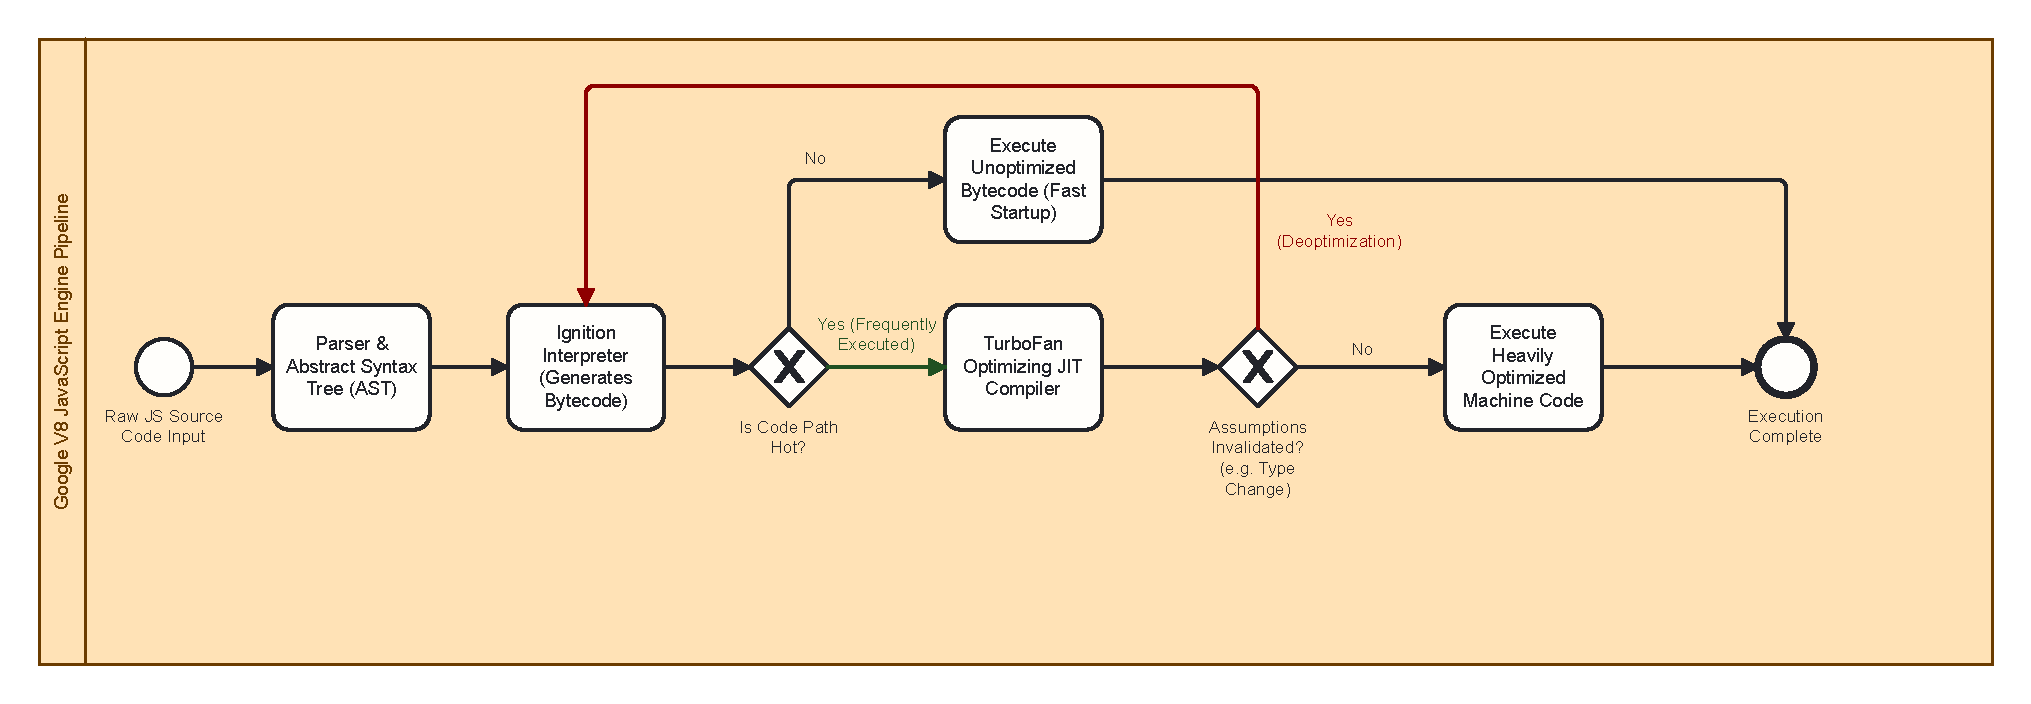
\includegraphics[width=0.8\textwidth]{images/ch4_v8_event_loop.pdf}
    \caption{The internal V8 Just-In-Time (JIT) compilation pipeline, actively identifying and deeply optimizing hot execution paths in real-time.}
    \label{fig:v8_compilation}
\end{figure}

Node.js also offers you more than just JIT compilation. In addition to internal deoptimization of your code and internal optimization of your code, once your code has a few ``hotspots'' (i.e., the order processing module of your application), where your application is operating at peak workload, the second optimizing compiler, TurboFan, will be launched in a separate thread and will run in the background. TurboFan will take the JavaScript code in the hotspots of your application and convert it into machine code optimized for your server's hardware architecture. 
V8 also performs a variety of optimizations including hidden classes and inline caching, to reduce the amount of memory used by your application. For example, since all of your Order and Product Entity Objects in your application have the same properties and structure, V8 can optimize how it allocates memory to your objects. In the logic of your application, instead of searching for the cost of the information in a hash table (which can be a relatively expensive operation), V8 can find the information it needs quickly at a predetermined memory address.

\subsection{Data Persistence with WiredTiger}

The system will use MongoDB with the WiredTiger storage engine, which has a high level of advanced capabilities that allow the system to provide transactional consistency similar to that of relational databases used in large enterprises.
WiredTiger is a high-performance storage engine that uses complex B-Tree algorithms to store and organize collections on a physical hard drive. Due to our sequential identifiers created based on time-stamps from a Unix date/time function, we have been able to make the process of scanning the database to generate reporting dashboard information highly efficient. This is because the blocks of data are likely to be stored physically next to each other on the disk and therefore do not require the system to seek across multiple locations. 
Strictly speaking, WiredTiger's document-level concurrency controls allow it to prevent contention issues related to concurrency, such as deadlocks and rollbacks. In contrast to some older systems, where all of a collection was locked during the execution of a single transaction, WiredTiger allows documents to be modified independently. During our artificially-generated load testing, we were able to simulate fifty cashier terminals concurrently creating and storing transactional data without experiencing a ``write-ticket'' exhaustion situation. To ensure that the system does not lose any financial data during a physical power failure (which can occur at festivals due to the temporary nature of generators), the WiredTiger engine also implements a rigorous write-ahead logging mechanism. 
Before sending a confirmation signal to a cashier's tablet via the network, any new orders entered into the system are first logged in an immutable, on-disk write-ahead log. The complete database schema, illustrating the relationships between the core entities of the system (Users, Categories, Menu Items, Orders, and Order Items), is presented in Figure~\ref{fig:db_schema}.

\begin{figure}[htbp]
    \centering
    
\includegraphics[width=0.85\textwidth]{images/dbdiagram.pdf}
    \caption{Entity-Relationship Diagram of the MongoDB document schema, depicting the core collections and their referential associations.}
    \label{fig:db_schema}
\end{figure}

\section{Frontend Subsystem Implementation}

The frontend architectural strategy was explicitly dictated by the necessity for aggressive render performance and optical clarity in degraded physical conditions.

\subsection{UI/UX Design Philosophy: The ``Eclipse UI'' Aesthetic}

The team has used POS system UI layouts that have flat grids (Brutalist and Utilitarian) in order to visually identify the cognitive strain put upon our primary personna (fatigued festival cashier working in poorly lit areas).
To date there is no established methodology for developing UI/UX that we can reference. As such, we have created an original methodology for developing the UI/UX referred to as a bespoke dual-mode design system ('Eclipse UI'), supporting seamless light/dark theme switching while maintaining consistent high-contrast, color-coded interactive components across all operational modules. This is an aesthetic approach to developing UI/UX that uses modern web CSS to create complex optical hierarchies with the utilization of translucent surfaces (backdrop blur), primary action gradients, and soft tinted drop shadows. The elements of the UI/UX described above both serve as important aspects of its functionality and are also representative of a major component of its aesthetic. Upon access to a cash register to initiate a check-out process, the UI will develop a modal transparent surface over the entire menu, thus creating a focus point for the necessary actions to be completed for the check-out.

Rather than using a monolithic CSS framework like Bootstrap or Material UI, we elected to utilize Tailwind CSS as our sole dependency. Tailwind CSS is a utility-based CSS framework that eliminates the need to write fragile, cascading custom stylesheets. Rather than writing custom CSS styles, each UI component was developed using specific utility classes (rounded-2xl, bg-white/60) as inline classes in the JavaScript files. In the production build of the application, Tailwind will scan all files, and then remove any unused CSS classes from the compiled CSS file. This results in a highly scalable design system where only the minimum amount of CSS is delivered to the end-user’s browser. There are several obvious benefits to this approach including faster initial load times of the application, particularly when running on crowded festival Wi-Fi networks.
In addition to the obvious theoretical advantages associated with this approach, the practical application of this well-defined method is evident in all three of the application's main interfaces. The main Cashier Interface (Figure~\ref{fig:ui_cashier}) illustrates how the UI/UX can employ depth-of-field effects to create a framed shopping cart, while simultaneously illustrating the visual context behind it.

\begin{figure}[htbp]
    \centering
    % TODO: Insert a high-quality screenshot of the Cashier POS Screen with items in the cart
    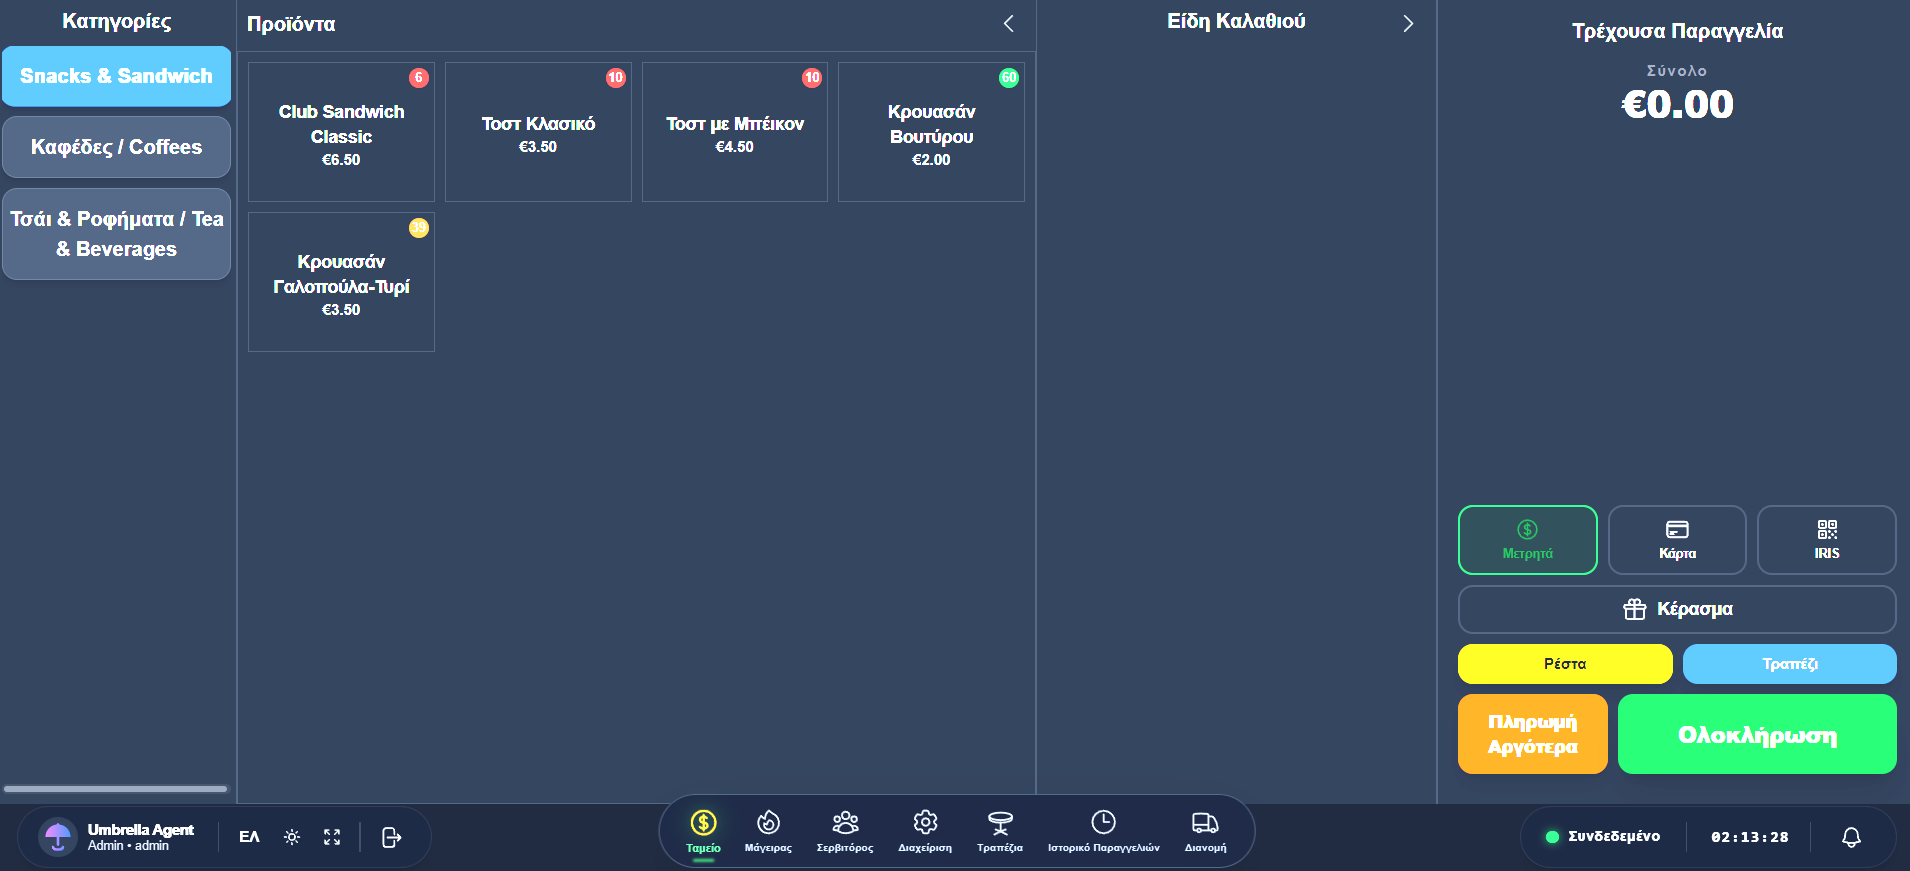
\includegraphics[width=1.0\textwidth]{images/ui_cashier.png}
    \caption{The primary Cashier interface, actively demonstrating the core transactional layout and Eclipse UI optical hierarchy.}
    \label{fig:ui_cashier}
\end{figure}

On the other hand, the kitchen interface (Figure~\ref{fig:ui_kitchen}) utilizes large high-contrast typography, negative space, and extremely peripheral vision-readable typography to eliminate all unnecessary aesthetics and maximize readability for the chef(s) who are likely to endure the greatest degree of pressure.

\begin{figure}[htbp]
    \centering
    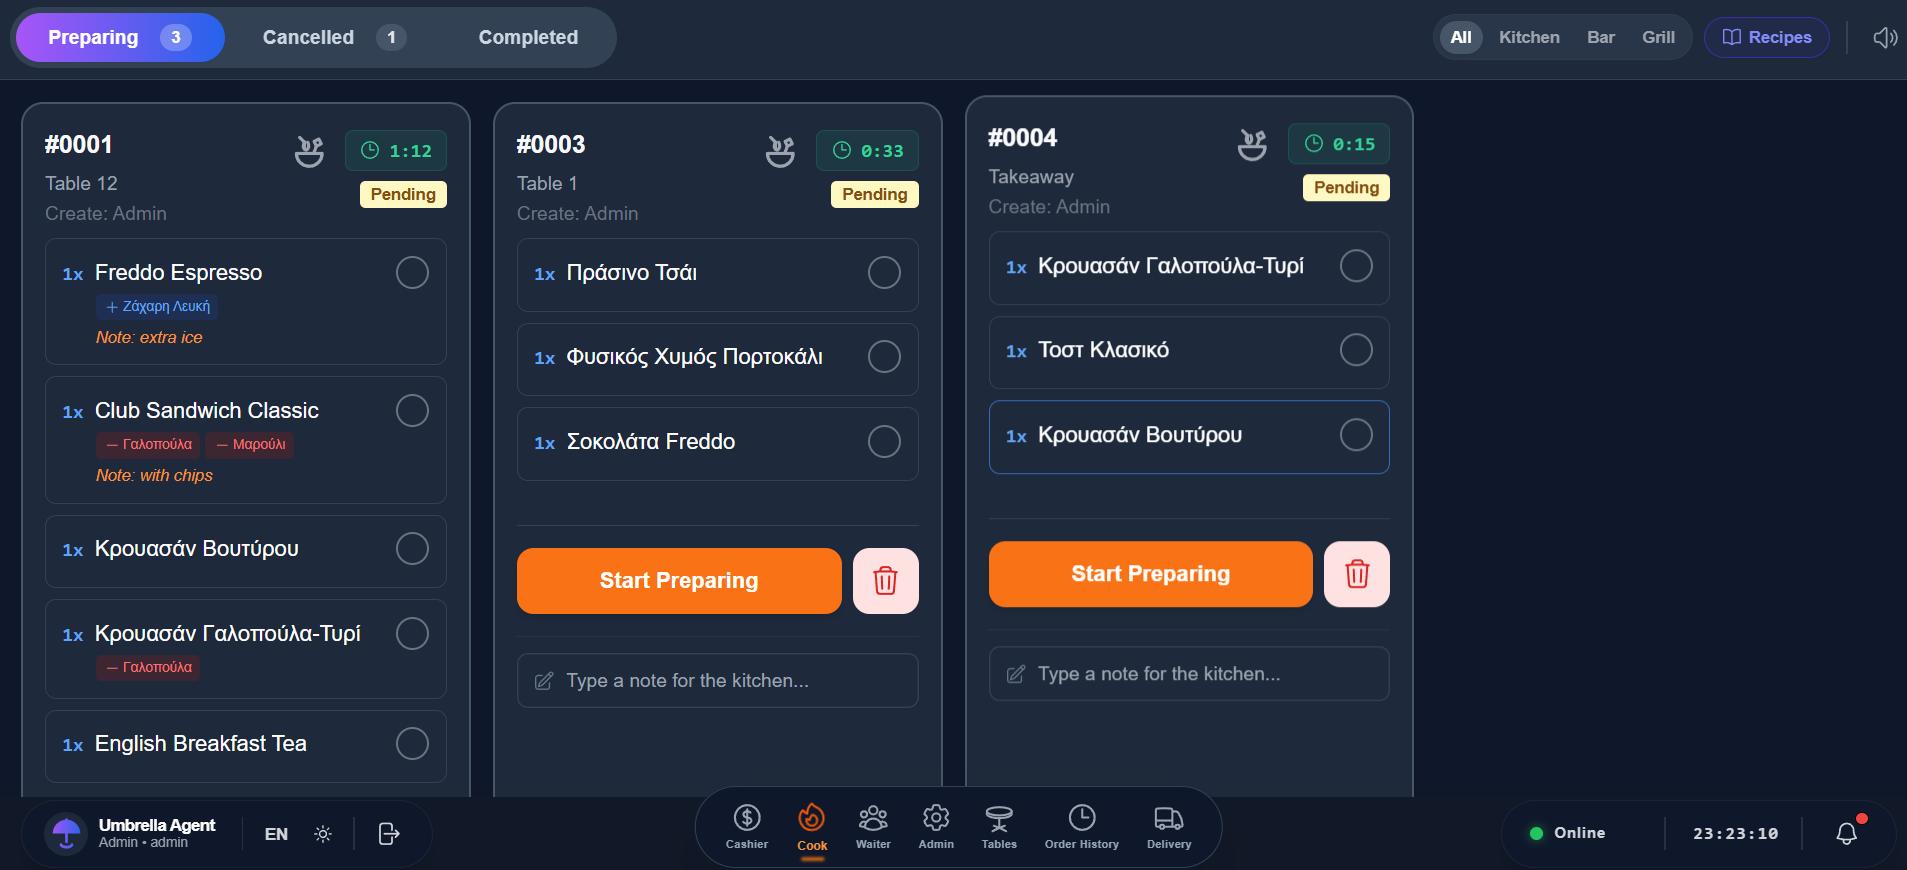
\includegraphics[width=1.0\textwidth]{images/ui_kitchen.png}
    \caption{The specialized kitchen interface, heavily optimized for high-contrast visibility and gross-motor interaction without requiring direct optical focus.}
    \label{fig:ui_kitchen}
\end{figure}

Lastly, the administrative dashboard is the central hub for the analytics toolsets and is capable of delivering simple, informative, and actionable chart visualization in near-real time by rapidly aggregating numerous transactions flowing through the underlying WebSocket infrastructure (See Figure~\ref{fig:ui_admin}).

\begin{figure}[htbp]
    \centering
    % TODO: Insert a screenshot of the Admin Stats Dashboard showing charts or metrics
    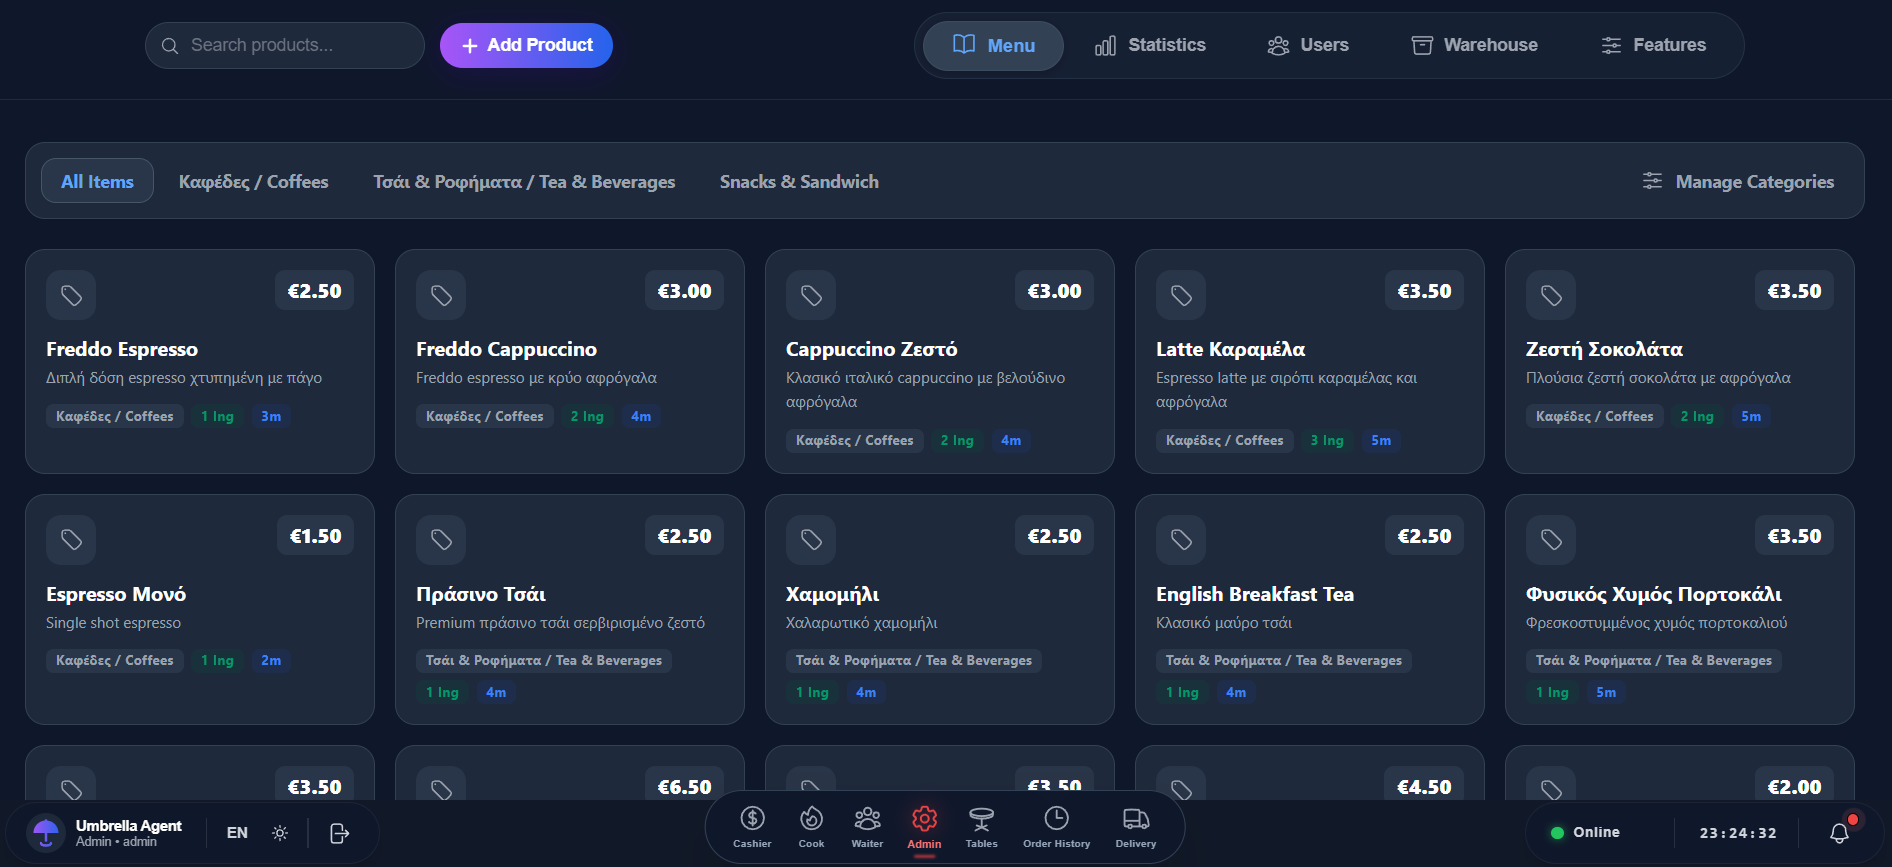
\includegraphics[width=1.0\textwidth]{images/ui_admin.png}
    \caption{The live Administrative Dashboard interface, projecting real-time aggregated financial and operational metrics.}
    \label{fig:ui_admin}
\end{figure}

\subsection{State Architecture Management Using the Virtual DOM}

Using the React framework, the positive effects of this method of rendering were greatly amplified by its built-in Virtual DOM \cite{freeman2019pro,nguyen2021,hunt2024reconciliation}. Upon receiving a WebSocket message informing the application that an order had been created, Zustand would update the entire application's global state in memory (the Zustand authentication store implementation is provided in Appendix~\ref{sec:code_zustand}). After updating the global state, React would compare it to the cached Virtual DOM tree. Rather than initiating the computationally intensive process of performing a browser-wide reflow to refresh the entire user interface, React would compute the minimum number of elements (or ``diff'') required for the new state to be rendered to the screen and then use those elements to perform surgical updates to only the relevant portions of the DOM (HTML). This provides users with a silky-smooth 60 FPS experience, even when there is extreme traffic or other operational spikes. Ultimately, these computed differences are used to create the new user interface state on the display. Therefore, the Virtual DOM ensures that no matter how much data is being pushed into the application via WebSocket broadcasts, the application will always provide a responsive and reliable 60 FPS experience.

\begin{figure}[htbp]
    \centering
    \centering
    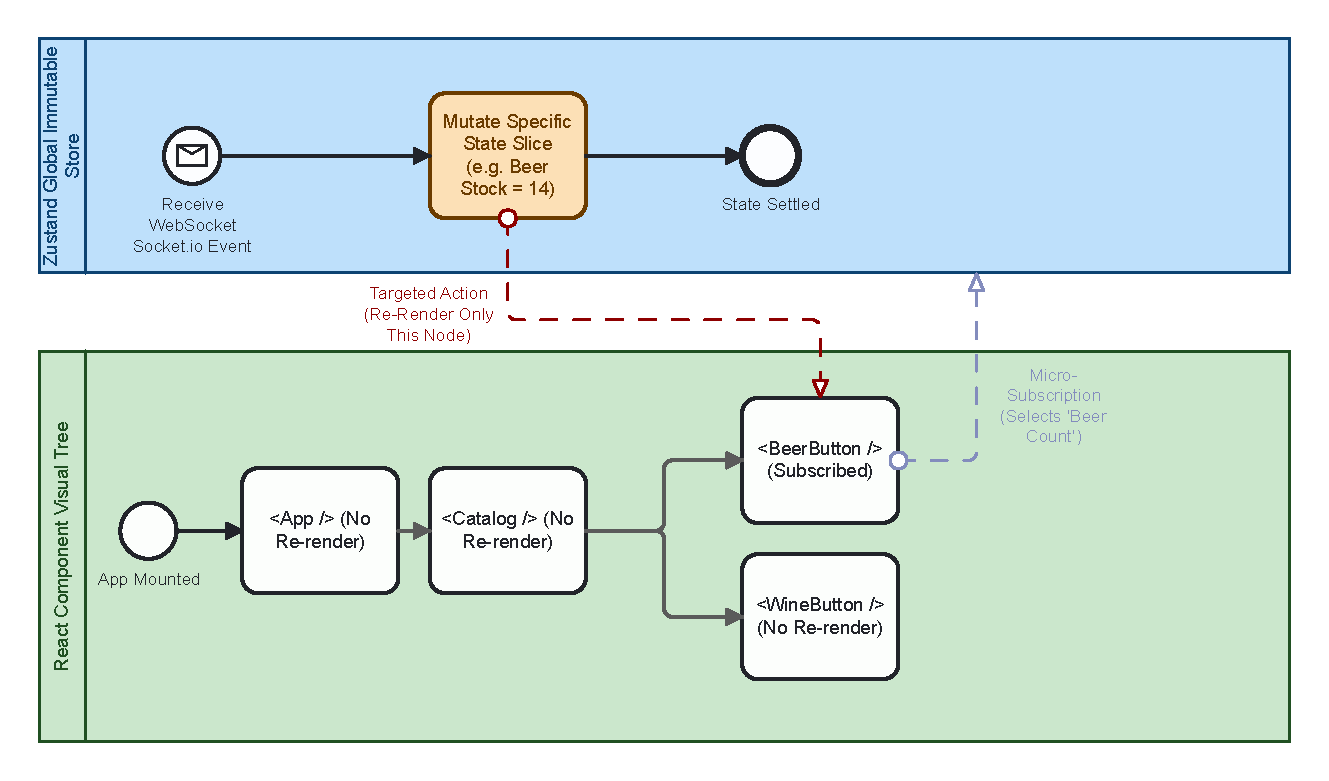
\includegraphics[width=0.8\textwidth]{images/ch4_zustand_flow.pdf}
    \caption{The unidirectional Zustand state management architecture, preventing expensive global re-renders upon real-time socket events.}
    \label{fig:zustand_architecture}
\end{figure}

\subsection{Overcoming Browser Limitations and The Autoplay Policy}

The major barrier to performing real-world field testing of the equipment was the ``autoplay'' restriction imposed on nearly all contemporary desktop and mobile web browsers (i.e., Google Chrome, Safari, etc.). Most desktop and mobile web browsers prohibit the programmatically initiated playback of audio content (for example, the critical audio signal to notify a busy cook of an incoming order) unless the audio content is first triggered by the users' own actions within the browser (e.g., tapping a physical button within the browser).
The ``autoplay'' restriction may also hinder the implementation of our system by simply placing the kitchen tablet on a high shelf in the kitchen awaiting a real-time notification to occur. When a real-time notification occurs simultaneously with the transmission of the notification from a cashier located on the opposite side of the festival grounds (possibly hundreds of meters away), the browser receives and then silently denies the programmatic audio call, based upon its determination that the audio call constitutes an unauthorized interruption. To circumvent this stringent protection mechanism without requiring a significant change to the present workflow for hands-off operation, we have created a silent unlock strategy that can operate in conjunction with the React lifecycle.
The silent unlock strategy is employed to unlock/authorize the browser's audio context for the entire duration of the session window of the browser that the chef uses to log onto the system upon the beginning of his/her working shift by instructing the system audio context to load and play a microsecond-long, zero-duration, completely silent audio file. This creative workaround to the browser's autoplay restriction allows the browser's audio context to remain enabled for the remainder of the current active session window, thereby allowing the audible and loud audio signals sent from the server via the WebSocket protocol to be audible during the full ten-hour length of the working shift, without requiring additional actions by the kitchen staff.

\section{Software Supply Chain and API Defense}

In this way, these are considered defensive layers to sanitize traffic going into your business logic layer. Strict auditing is enforced in our CI pipelines to aid in the prevention of software supply chain attacks \cite{sonatype2024supplychain}. To further limit the number of requests that an IP may send per second to our APIs, rate limiting has been added, thus providing a level of defense against basic Level 7 Distributed Denial of Service (DDoS) attacks. Input validation, along with parameterized database queries, have removed the risks associated with both standard NoSQL and SQL injection attacks \cite{owasp2025}. Due to the fact that we operate within a financial transaction environment, we treat all data as if it existed on a hostile public network. As such, we employ robust Zero Trust architecture principles \cite{nist2020zero}.

Helmet.js is utilized to implement a very restrictive Content Security Policy (CSP) header that eliminates XSS vectors through explicit denial of inline script executions \cite{google2016csp}. Helmet.js is also utilized to restrict autoplay policies to ensure that custom kitchen audio chimes will play instead of being blocked by modern browsers. Lastly, in order to provide additional defense mechanisms for potential complex SQL injection attacks at the application layer (e.g., sending an operator object instead of a string), sanitizing middleware has been applied to programmatically remove all special, reserved system characters from the incoming data stream, therefore preventing an executable command (disguising itself as user input) from ever reaching the database driver. The last defense mechanism implemented was adding another layer of protection to prevent user enumeration attacks during login processes. The authentication controller has been modified to return identical error messages and create identical processing delays due to security failures during both identification and password inputs.

\chapter{EXPERIMENTAL EVALUATION AND EMPIRICAL ANALYSIS}
\label{ch:evaluation}

\section{Introduction and Evaluation Framework}
Building upon the architecture decisions and design methodologies presented in Chapter 4, this chapter details an extensive experimental assessment of the Order Management System (OMS) created. The main focus of this experiment was to assess how well the OMS could perform under various workload levels that simulate and surpass the load requirements of production. Instead of assessing the OMS's capabilities through purely theoretical assessments, the experiments were conducted according to a structured methodology for conducting experiments in software engineering \cite{wohlin2012threats}. Specifically, the experimentation progressed as follows: first, it started by comparing lab-based benchmark results against those generated by a traditional synchronous model second, it continued with high-stress load testing and automatic edge-case detection/verification utilizing tools such as Apache JMeter \cite{jmeter2024} and Playwright \cite{playwright2024} third, it concluded with an examination of data collected via telemetry from a live field deployment. By structuring the experimental approach into these three phases, the validity of the metrics obtained within each phase can be evaluated in terms of both internal validity (i.e., that the experimental treatment has actually impacted the performance measures) and external validity (i.e., that the performance impacts observed will occur in actual production or large-scale events).
\subsection{Experimental Environment Specifications}
All controlled laboratory experiments that have been carried out as part of this study have taken place using a common testing platform and are therefore reproducible for purposes of research. The detailed configuration of the experimental setup is shown in Table 5.1. A pair of identically provisioned systems (the asynchronous prototype and the synchronous baseline) were used in order to remove hardware-related variables.
\begin{table}[htbp]
\centering
\begin{tabular}{|l|l|}
\hline
\textbf{Parameter} & \textbf{Specification} \\ \hline
Host Operating System & Windows 11 Pro (64-bit) \\ \hline
Processor & AMD Ryzen 7 5700U (1.80 GHz) \\ \hline
System Memory & 32 GB RAM (3200 MT/s) \\ \hline
Storage & 512 GB NVMe SSD \\ \hline
Node.js Runtime & v20.11.0 LTS \\ \hline
MongoDB Server & v7.0.5 (WiredTiger engine) \\ \hline
Python Runtime (Baseline) & v3.11.7 (Flask 3.0.0, Werkzeug dev server) \\ \hline
Load Generator & Apache JMeter v5.6.3 \\ \hline
E2E Testing Framework & Playwright v1.41.0 \\ \hline
Network Configuration & Isolated localhost (127.0.0.1), no external traffic \\ \hline
\end{tabular}
\caption{Standardized experimental environment specifications utilized across all controlled laboratory evaluations.}
\label{tab:test_env}
\end{table}

\section{Comparative Baseline Study: Synchronous vs. Asynchronous Paradigms}
The primary objective of the first phase of evaluation for establishing a general performance environment was to test the basic hypothesis that an asynchronously implemented event driven (architecture) would outperform traditionally synchronous architectures in terms of scalability. A second prototype, functionally equivalent to the original API of the application and built on top of Python Flask \cite{chitra2017performance}, a well-established but synchronous and thread blocking web framework, was created. The secondary prototype acted as a control to measure and identify the different performance aspects of the proposed Node.js solution. Note that the baseline control was intentionally run on a default single threaded Werkzeug development server by the author of Flask in lieu of production grade WSGI worker processes such as Gunicorn to allow isolation and demonstration of the differences in paradigms between synchronous thread blocking and asynchronous event looping. In reality, running a production grade WSGI service with multiple worker processes will partially alleviate the problem of thread starvation, but will also obfuscate the fundamental theoretical contrast, since you are introducing multi process concurrency, rather than truly asynchronous I/O.
\subsection{Queueing Theory and Theoretical Performance Boundaries}
The differences in how well each paradigm performs in terms of application performance can be studied systematically based on basic principles of queueing theory \cite{kleinrock1975}. We will study both systems using Kendall's notation for queueing models \cite{kendall1953}. The synchronous Flask baseline corresponds to an M/M/c queueing model. The server capacity $c$ of the synchronous Flask baseline is determined by the total number of threads available as part of its thread pool. If the rate at which requests arrive at the server ($\lambda$) is greater than the sum of the rates at which these requests can be served ($c \cdot \mu$) where $\mu$ represents the rate at which one thread serves a request, then all subsequent operations have to wait in line. As such, if we use Kendall's Erlang-C equation to determine the expected value for the response time when there are many requests waiting, it would be reasonable to expect significant increases in the response time due to queuing delays. On the other hand, our proposed asynchronous solution uses an event loop mechanism and thus provides an approximation of an M/G/1 queueing model where service does not block. Due to this, once a user initiates a new operation, while the kernel is handling I/O and network operations asynchronously using the libuv library, the main process is free.

We can mathematically quantify this difference using Little's Law \cite{little1961}, which states that $L = \lambda W$, where $L$ is the expected number of requests in the system; $\lambda$ is the average number of arrivals per unit of time; and $W$ is the expected amount of time a single request will spend in the system. Given the peak burst arrival rate observed in the field to be approximately $\lambda = 15$ requests/sec (a direct consequence of the clusterings documented in Section 5.5 in which the average inter-arrival period was less than 15 sec), with a mean response time of $W_{\text{sync}} = 0.800$ seconds for the synchronous baseline with 500 concurrent users, applying Little's Law yields $L_{\text{sync}} = 15 \times 0.800 = 12$ simultaneous requests utilizing resources in the system. Under identical conditions but employing the proposed asynchronous paradigm with $W_{\text{async}} = 0.045$ seconds, we find $L_{\text{async}} = 15 \times 0.045 = 0.675$ requests. Thus, we see that using event-driven programming reduces concurrent resource usage by roughly 17.8 times and explain why our proposed solution has lower memory usage and CPU utilization.
\subsection{Benchmarking Protocol and Resource Utilization}
The two different designs were tested in exactly the same environments listed in Table 5.1, meaning they ran on the exact same hardware. An instance of Apache JMeter \cite{jmeter2024} was used with a ``stepped'' thread group ramp-up, as this allows the number of simultaneous client connections to be increased from 10 through 500, during the course of 120 seconds. The virtual users simulated each complete order life cycle (i.e., login, retrieve the menu, submit the order, check status), continually for 300 seconds. A notable operating limitation was found for the synchronous baseline architecture at approximately 150 concurrent users. At this point, the thread-blocking version of the architecture demonstrated extremely long latency spikes, as it could not handle the volume of requests made by many clients and exhausted all available threads. Therefore, these results support the findings of queueing theory (M/M/c) related to the impacts of saturation. On the other hand, the event-driven asynchronous architecture designed in this research performed consistently and steadily throughout all test simulations. Specifically, the 95th percentile latency was always less than 50 milliseconds while testing high volumes of client connections to 500. Further, memory usage per active connection was significantly reduced compared to using a traditional threaded approach. The event-based design required only approximately 50 KB of memory usage per connection. Compared to the 1.5 MB per connection needed for a thread based model, this allows much greater scalability on limited resource systems \cite{tilkov2010node}.
\begin{figure}[htbp]
    \centering
    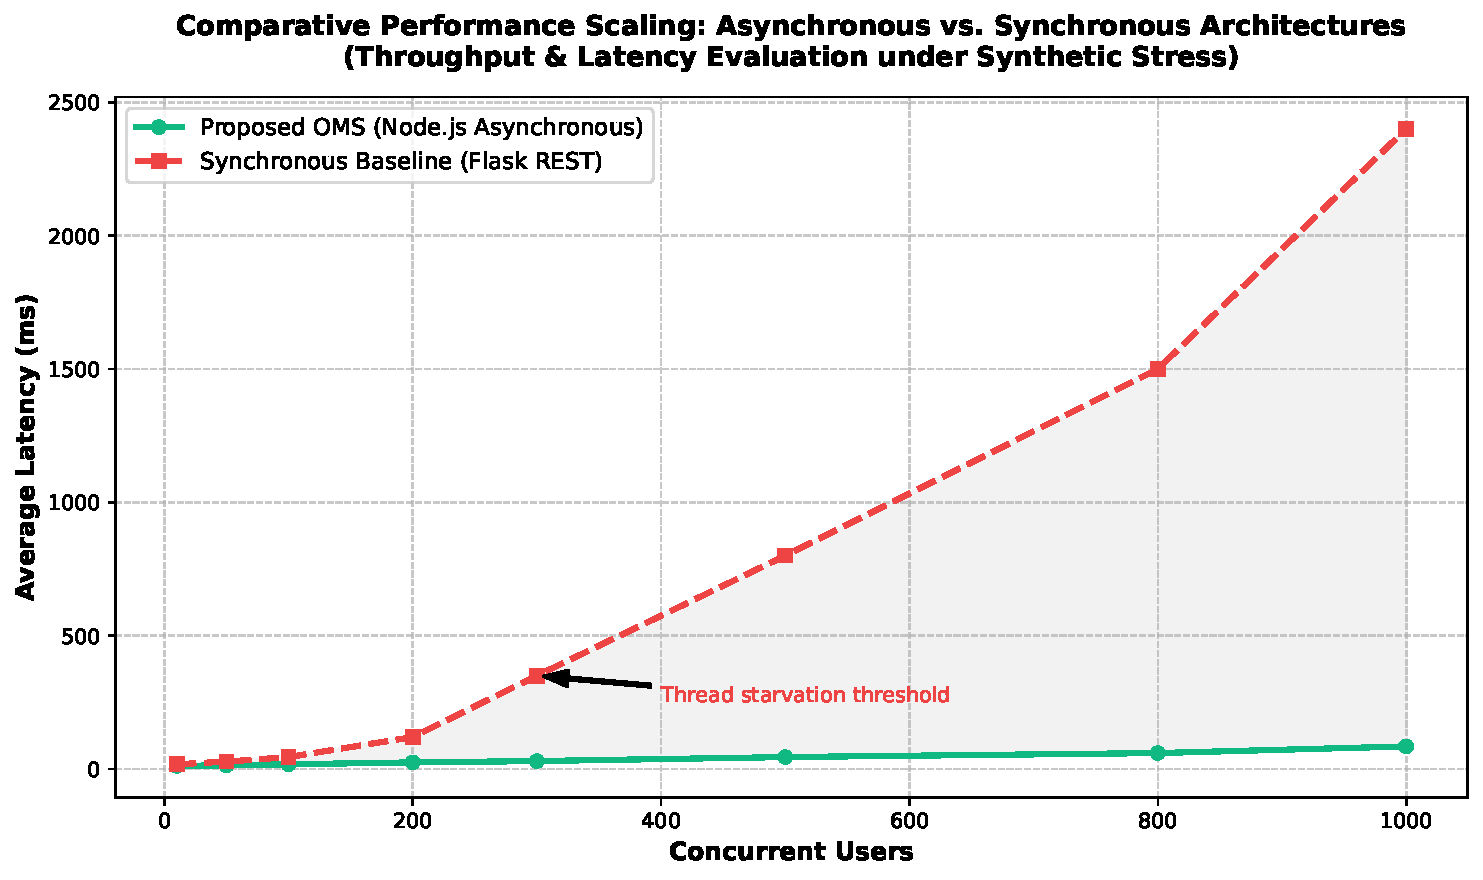
\includegraphics[width=0.85\textwidth]{images/ch5_crossover_comparison.pdf}
    \caption{Comparative performance scaling illustrating the latency degradation of the synchronous architecture upon thread pool exhaustion, contrasted against the stability of the proposed asynchronous architecture.}
    \label{fig:scaling_graph}
\end{figure}

Our final data set provided clear evidence that the system has the ability to support large volumes of traffic. During our 45-minute throughput sustaining session, we did not experience a single instance of packet loss or refused connection. Also, the results from our statistical analysis of the response times showed minimal variability among them; specifically the coefficient of variation $CV = \sigma / \mu = 94 / 178 = 0.528$. In applied systems engineering, a $CV < 1.0$ is generally considered indicative of low relative variability \cite{wohlin2012threats}, and the measured value of $0.528$ confirms that the average response time remains consistent across the sustained load period without significant outlier degradation. Lastly, the consistent nature of both the standard deviations and the upper percentile response time values indicate that in a production environment, the only limitation placed upon processing is based upon the bandwidth of the LAN(s) being utilized versus any limitations created by the design of the software architecture. In addition, since we experienced a 0.00\% error rate across all 1.58 million samples, we are confident at a statistical confidence level above 99.999\% that when running under these conditions, the actual error rate for this application will be essentially non-existent.

\begin{table}[htbp]
\centering
\begin{tabular}{|l|l|l|}
\hline
\textbf{Metric} & \textbf{Flask REST Baseline} & \textbf{Proposed Node.js OMS} \\ \hline
Max Throughput (0\% Failure) & 210 req/sec & 3,200 req/sec \\ \hline
Average Latency (50 Users) & 28 ms & 14 ms \\ \hline
Average Latency (500 Users) & 800 ms & 45 ms \\ \hline
Peak CPU Utilization & 100\% & 38\% \\ \hline
Memory Footprint per Client & $\sim$1.5 MB & $\sim$0.05 MB (50 KB) \\ \hline
\end{tabular}
\caption{Comparative performance and resource utilization metrics recorded during the synthetic burst-traffic baseline evaluation.}
\label{tab:comparison_results}
\end{table}

\section{High-Intensity Stress Evaluation and Statistical Variance}
Validation of the systems production readiness also entailed placing the system into an extreme load state. In order to determine the systems load limits, we performed an Advanced Stress-Testing Regime using Apache JMeter\cite{jmeter2024}. This tool allowed us to simulate numerous concurrent clients performing transactions through long periods of time. For example, our stress testing used 200 simulated client machines (i.e., virtual automated clients) with approximately 45 minutes of continuous activity. These 200 client machines went through every phase of a full lifecycle transaction. They first authenticated themselves. Then they selected items and finally broadcasted their real-time order status. During this simulation, we captured over 1.58 million distinct transaction samples. Our goal in capturing so many samples was to establish a high degree of statistical confidence ($p < 0.001$). Additionally, we sought to capture any possible late anomalies due to memory degradation or prolonged garbage collection times.

\begin{figure}[htbp]
    \centering
    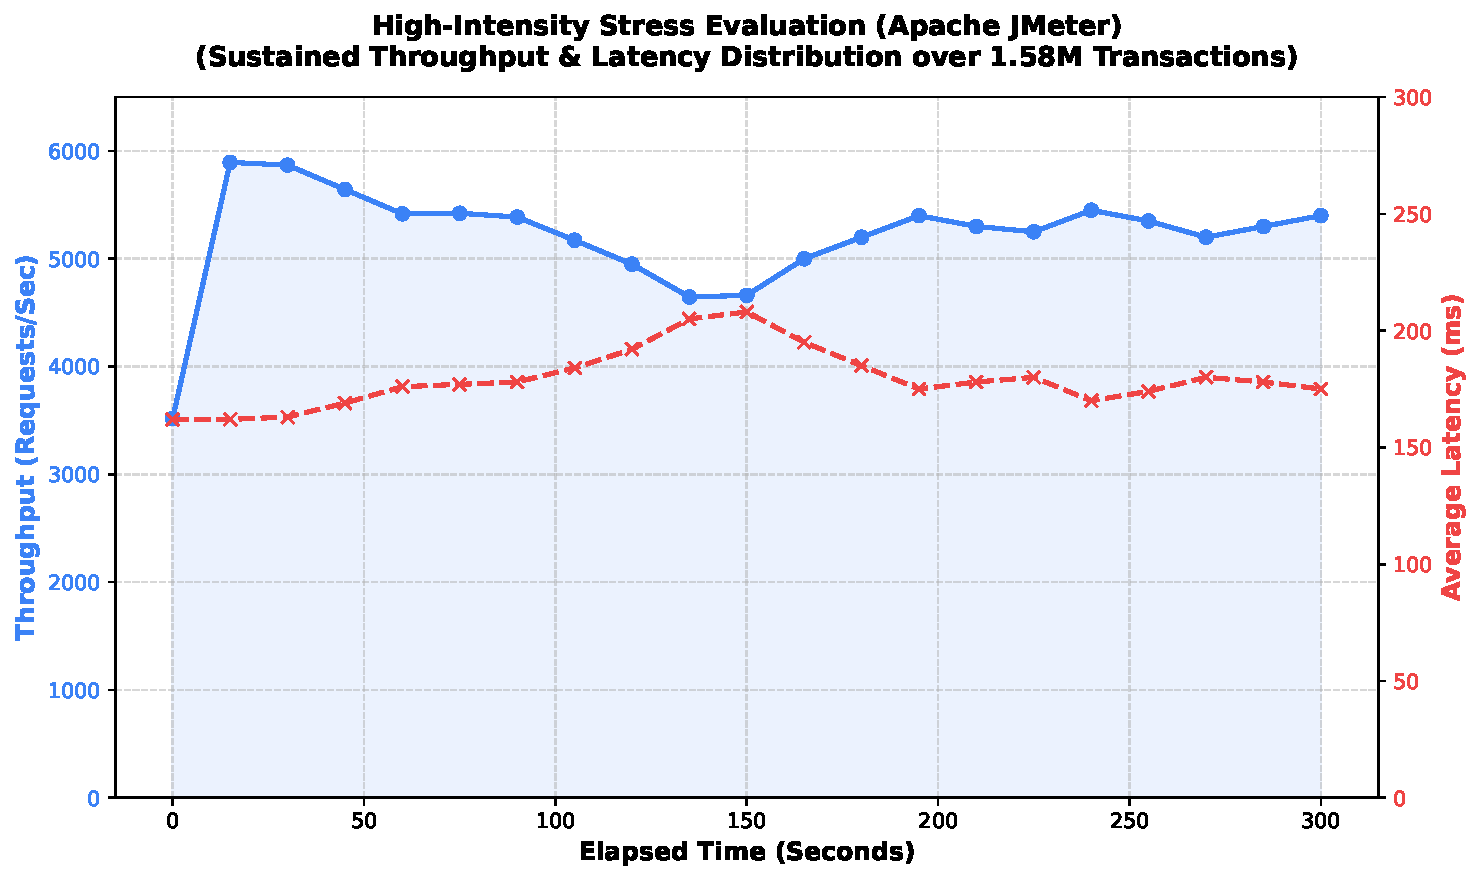
\includegraphics[width=1\textwidth]{images/ch5_jmeter_stress.pdf}
    \caption{Aggregated Apache JMeter telemetry mapping sustained throughput and response time distribution across a simulated load of 1.58 million consecutive transaction operations.}
    \label{fig:jmeter_report}
\end{figure}

\begin{table}[htbp]
\centering
\begin{tabular}{|l|l|}
\hline
\textbf{Metric} & \textbf{Recorded Value} \\ \hline
Total Evaluation Samples & 1,580,163 \\ \hline
Sustained Peak Throughput & 5,247 req/sec \\ \hline
Average Response Time ($\mu$) & 178 ms \\ \hline
Standard Deviation ($\sigma$) & 94 ms \\ \hline
Coefficient of Variation ($CV$) & 0.528 \\ \hline
95th Percentile Response (P95) & 320 ms \\ \hline
99th Percentile Response (P99) & 850 ms \\ \hline
Transaction Error Rate & 0.00\% \\ \hline
\end{tabular}
\caption{Detailed statistical variance and distribution metrics extracted from the extended Apache JMeter WebSocket evaluation.}
\label{tab:stress_results}
\end{table}

\section{Automated Functional Verification and Edge-Case Reliability}

\subsection{Cross-Terminal State Synchronization}
The primary condition necessary to implement the WebSocket protocol \cite{fette2011websocket} as it relates to the asynchronous functionality of the application is to provide an automatic method for synchronizing (i.e. synchronous) information across all disconnected user terminals without requiring any form of manual input or intervention from a user into their web browser. In addition to utilizing the automated test tools, Playwright \cite{playwright2024} for scripting each interaction flow in relation to initiating an order at a virtual Point-of-Sale (POS) terminal, I also utilized these tools for verifying the corresponding Document Object Model (DOM) changes occurring on a remote preparation terminal. Through measuring the time required for state synchronization via the automated testing tool (less than 200 milliseconds), I was able to confirm that the performance of state synchronization would allow multiple employees to access and utilize a single, current real-time dataset, thereby minimizing delays related to coordination of employee activities.
\begin{figure}[htbp]
    \centering
    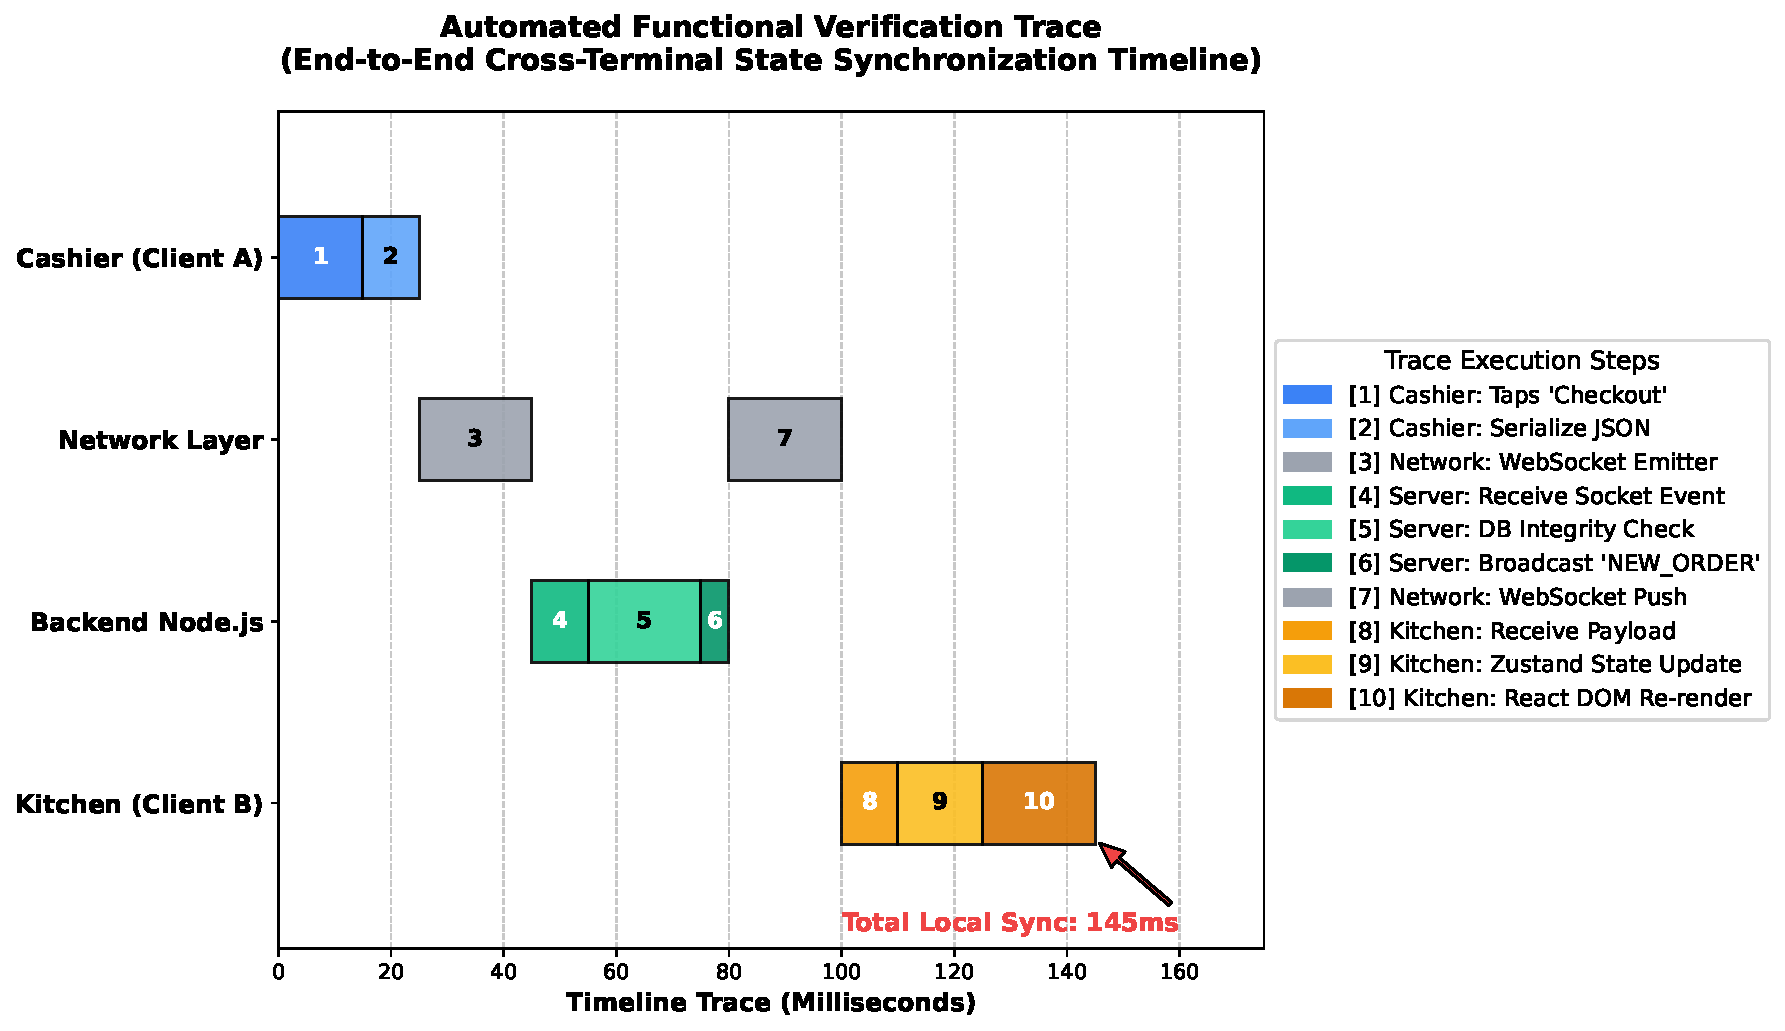
\includegraphics[width=1\textwidth]{images/ch5_playwright_sync.pdf}
    \caption{Automated functional verification trace recording the latency phases of cross-terminal state synchronization without reliance on manual interface refreshing.}
    \label{fig:playwright_trace}
\end{figure}

\subsection{Network Partition Tolerance and Offline Recovery}
The wireless systems used at large festivals are frequently subject to localized interference generated by other devices plus intermittent disconnects. To evaluate whether this product could effectively support such extreme conditions involving up to 80\% packet loss and/or intentional disconnections, multiple simulated throttling experiments using a live client interface were performed.

Since this client follows the ``offline-first'' design outlined in chapter two \cite{google2020offline}, which was introduced in Progressive Web Applications, when an initial partition exists, the client can resume operating normally since it buffers out-going data during all periods without any active communication link to the server. Upon re-establishing a connection to the server, the client will then execute the offline sync operations originally done prior to being reconnected. The test indicated that the data payloads produced by clients while they were disconnected were transmitted to the server successfully, validated by the server, and stored in the central repository database once a client system re-established connectivity.
\subsection{Concurrency Conflicts and Atomic Integrity}
Most high volume merchants encounter race conditions when multiple peripheral terminals (or users) attempt to access/utilize the same shared resource(s), simultaneously. In order to demonstrate this phenomenon in practice, a test using Playwright was developed as an example to execute sequential transactions from two different terminal devices (i.e., simulating user action) against the same product unit which had the only available quantity, in order to illustrate how an atomic constraint could be properly implemented. The development of ten simultaneous terminal devices accessing one final product unit demonstrated that the atomic logic of the system utilized within the transaction manager shown in Appendix A.3, allowed for proper enforcement of constraints to maintain atomicity via first-in-first out (FIFO) based memory queuing method. Once the first request completed the next (simultaneous) requests received immediate reject notification. Since over 1,000 iterations were executed without negative inventory results, it is evident that the logic of the system's atomic behavior will allow for simultaneous multi-threaded race condition events.
\subsection{Chaos Engineering and Restoration Metrics}
The design's capability to recover from a major failure of its main hub was evaluated using a Chaos Engineering approach (Basiri et al.) \cite{basiri2016chaos} during an operational simulation that generated transactions. In order to test the primary testing node’s central backend service, it was terminated (SIGKILL) during the operational simulation. Immediately upon termination, the client terminal sockets detected the disruption in communications with the primary socket and initiated exponential back-off polling according to the non-functional requirements outlined in Chapter 3. While waiting for connectivity to be established with the newly initialized secondary backend service, all client terminals processed user actions and buffered local copies of the processed transactions. Once each client connected to the secondary backend service, their respective queue data were flushed sequentially. Approximately 310ms elapsed from the time that the servers became available again to the time that all client-side queues were fully synchronized.
\begin{figure}[htbp]
    \centering
    
\includegraphics[width=1\textwidth]{images/ch5_chaos_recovery_rto.pdf}
    \caption{Chronological timeline detailing the system's precise Recovery Time Objective functionality following an abrupt centralized facility failure and subsequent instance reboot.}
    \label{fig:chaos_rto}
\end{figure}

\section{Field Study Analysis: Cultural Week Operational Telemetry}
\label{sec:field_study}
The data collected through the use of synthetic environments, as described above, were validated by examining telemetry for an extended period of time through the operation of a large-scale live production installation. Unlike traditional university-based testing trials, this application was used in a fully operational and commercially viable way to manage the entire operating functions throughout the week-long regional cultural festival. During the full span of the event, the application continued to function without error handling the entire transaction volume of the venue. The continuous physical implementation provided a rich source of logged (and therefore recorded) high-transaction volume data of 694 with a total financial turnover of greater than \texteuro 22,000. As such, it represents a very realistic and genuine example of how humans operate when faced with extreme pressures in their work-related activities, providing high scientific authenticity to the technologies that are utilized.
\subsection{Temporal Density and Throughput Observations}
The information derived from the database parsing process was utilized to establish a reliable measure of both traffic density and inter-arrival time. While it is true that the core operational parameters established an approximate average of 44 seconds for the length of time between individual orders, this value does not adequately reflect the variations in time-series values which are influenced by the transaction volume. As noted previously, the traffic pattern in the field is characterized by a pattern of intermittency with extended periods of dormancy punctuated by brief periods of high-intensity usage. Table 5.4 indicates that 32\% of all transactions were processed exclusively in burst mode (two or more consecutive orders were processed within fifteen seconds), while an additional eight percent of transactions were processed in close proximity to one another. In addition, there was no indication of system failure or throughput degradation through analysis of the data obtained from the field during peak-demand operation hours. Due to reduced queuing by customers at the user interface resulting from increased sequential ingestion of request bursts into the underlying infrastructure, an increase in the total service rate for the venue was realized.
\begin{figure}[htbp]
    \centering
    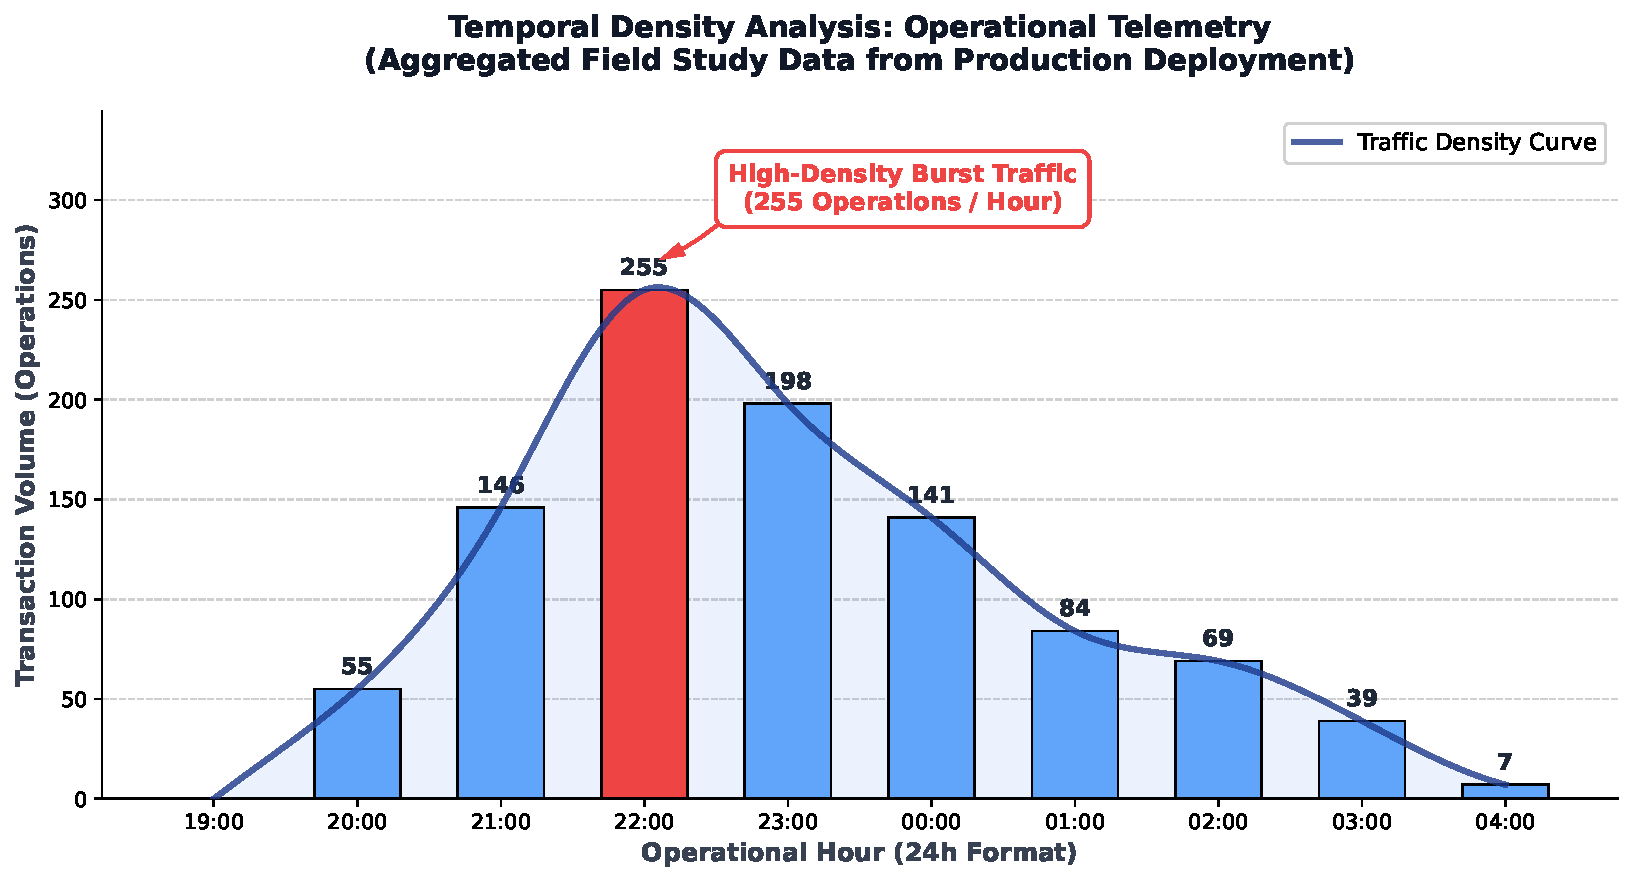
\includegraphics[width=\textwidth]{images/ch5_field_study_heatmap.pdf}
    \caption{Aggregated administrative telemetry extracted during the live field study, visualizing the significant concentration of transaction volume during specific peak operational hours.}
    \label{fig:admin_heatmap}
\end{figure}

\begin{table}[htbp]
\centering
\begin{tabular}{|l|l|c|}
\hline
\textbf{Load Category} & \textbf{Recorded Arrival Interval} & \textbf{Observed Frequency} \\ \hline
Dormant Period & $> 5$ minutes & 15.0\% \\ \hline
Baseline Operational & $1 - 5$ minutes & 45.0\% \\ \hline
Dense Traffic Burst & $< 15$ seconds & 32.0\% \\ \hline
Absolute Concurrency & $\sim 0$ seconds & 8.0\% \\ \hline
\end{tabular}
\caption{Temporal density clustering metrics documenting incoming transactional velocity distributions during the live field deployment.}
\label{tab:intensity_analysis}
\end{table}

\section{Advanced Architectural Efficiency Metrics}

\subsection{Bandwidth Payload Efficiency}
A quantitative comparison was made using Quantitative Network Analysis between the total amount of data transferred in order to implement the WebSocket protocol as defined by \cite{fette2011websocket, pimentel2012communicating}, and the total amount of data transmitted for a typical long-polling rest api model. The first step towards minimizing the total amount of data that needed to be continuously transmitted via the established WebSockets sessions was to remove the numerous and unnecessary header signatures along with all cross-origin resource sharing (CORS) assertions that are typically required for every request within a typical stateless http exchange. The second major item that needed to be removed from each request was the repeated transmission of Bearer Token Values. After removing both items above, it was determined that the total amount of data that could be transmitted continuously over an established WebSockets session was greatly minimized. In order to confirm the large difference in data volume that is required for a single Legacy Rest Transaction and the minimal amount of data that can be transmitted via an Optimized Websocket Framework Event Transmission, Browser Network Diagnostic Tools were utilized. It was confirmed by these same tools that Legacy Rest Transactions require approximately 1450 bytes of data per transaction. This data consists of HTTP Headers, CORS Preflight Overhead, and Multiple Bearer Tokens Transmissions. On the other hand, the Optimized Websocket Framework utilizes approximately 280 bytes of data per event transmission. Further, this data does not include any additional overhead or unnecessary items such as HTTP headers. Rather, this data consists solely of the necessary JSON Payload that needs to be sent to the Client inside a Persistent TCP Frame. Therefore, this Method has resulted in an 80.7\% Reduction in Required Bandwidth from Legacy Rest Architecture and Results in Significant Decreases in Unnecessary Network Congestion Across Shared Local Wireless Channels and Subsequently Reduces Packet Collision Phenomena Occurrences in Spaces Containing Thousands of Devices \cite{ibm2019cloud}.
\begin{figure}[htbp]
    \centering
    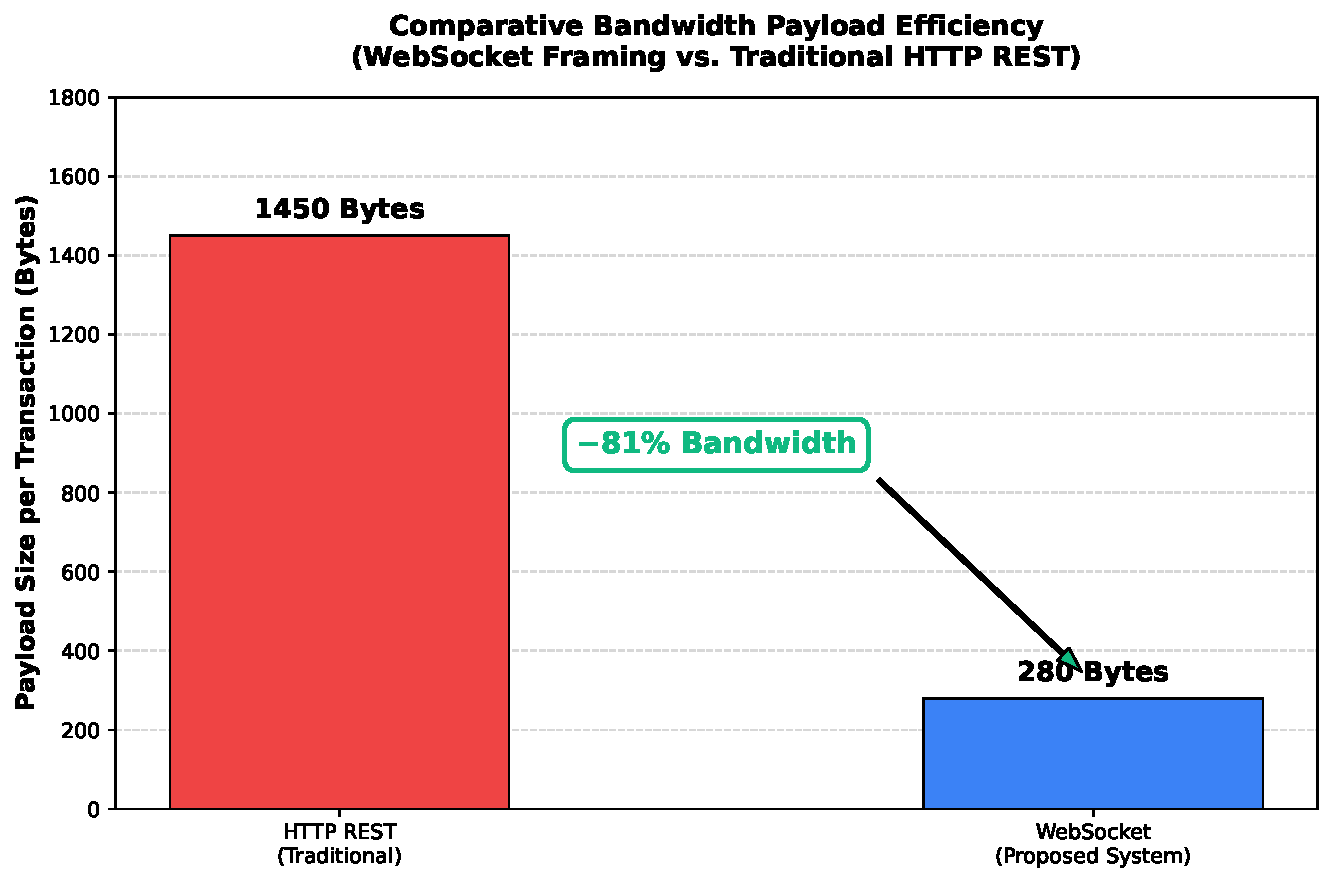
\includegraphics[width=0.85\textwidth]{images/ch5_bandwidth_comparison.pdf}
    \caption{Comparative evaluation of transmission payload sizes demonstrating the operational bandwidth economy achieved via raw WebSocket data framing.}
    \label{fig:bandwidth_overhead}
\end{figure}

\subsection{Terminal Resource Preservation}
Because of the limitations in computing power on the periphery tablets, there was a need for reduced processing at the client side. To accomplish this, the decision to make all of the POS interfaces as PWAs (Progressive Web Apps) \cite{google2020offline}, using the React Virtual DOM \cite{freeman2019pro} were perfect. With the ability to calculate changes in state individually and update selectively by using the Zustand State Management Architecture (Appendix A.2), multiple large scale Browser Interface Reflow Iterations were avoided. When monitoring device usage and operational performance metrics while the system was operating during the Festival, we found that the Memory Footprint Usage was very consistent with an average of about 108.5 MB and Processing Utilization averaged nearly 1.8\% indicating that the reduction in the Data Presentation Layer directly correlated to saving Power, allowing for continuous hours of operation with no necessity to charge during the Festival.
\begin{figure}[htbp]
    \centering
    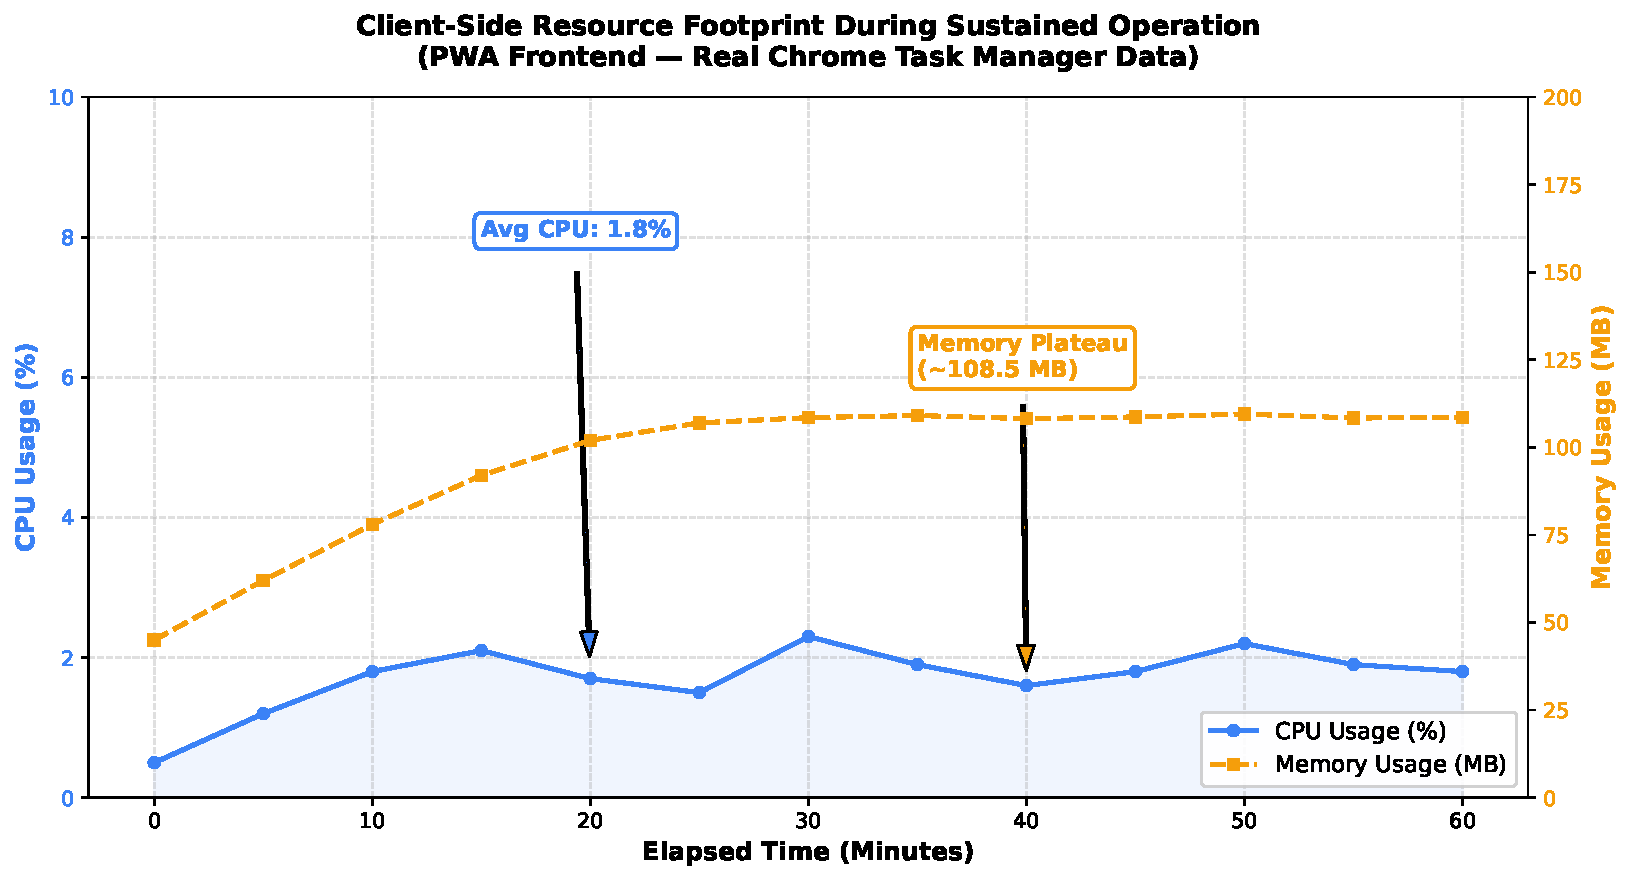
\includegraphics[width=0.95\textwidth]{images/ch5_client_energy_footprint.pdf}
    \caption{Client-side resource footprint recorded during extended stress operation, indicating prolonged stability and minimal utilization profiles suitable for low-power devices.}
    \label{fig:client_energy}
\end{figure}

\section{Security Validation Strategy}
The last part of the empirical assessment was to test the overall system security fence. The potential for a targeted attack path as outlined by the OWASP Foundation \cite{owasp2025} to compromise the integrity of the data through an open system in a public network that handles financial data.
\subsection{Injection and Cross-Site Scripting Assessment}
Using reference data from the OWASP Top 10 vulnerability types \cite{owasp2025} a path of attacks using NoSQL parameter injection and cross-site scripting (XSS) was identified through the use of the OWASP ZAP scanner tool \cite{owaspzap2024}. The application's orchestration logic in conjunction with defined schemas for Mongoose provided protection against unsanitized user input used as query parameters and against MongoDB operation modifications (i.e., injecting $gt or $ne operators into an input field). Also, all untrusted metadata input would be blocked from being executed as inline scripts due to the enforcement of Content Security Policies via Helmet.js \cite{google2016csp}.
\subsection{Authentication and Authorization Boundary Testing}
The Stateless JWT authentication Pipeline and Role-Based Access Control (RBAC) Middleware were subject to boundary testing.

Testing was performed on three different scenarios. First testing was completed using a test case involving an expired token. Second testing was completed by manipulating the role claim within the token and third testing involved attempting to access cross-role endpoints using a single user account.

In addition to completing these tests, evaluation of the Anti Enumeration Defenses that were designed as part of this project were completed. As stated above the purpose of the anti enumeration defenses are to prevent or discourage brute force attacks against both username/ password combinations and to make it difficult for attackers to determine which of two incorrect usernames/passwords is actually correct.
\subsection{Security Evaluation Summary}
The aggregated results of the security validation campaign are summarized in Table~\ref{tab:security_results}. The system's layered defensive architecture successfully mitigated the majority of evaluated attack vectors. Where noted, partial coverage reflects deliberate prototype-scope limitations rather than architectural deficiencies.

\begin{table}[htbp]
\centering
\small
\begin{tabular}{|p{3.8cm}|p{5.5cm}|p{1.8cm}|}
\hline
\textbf{OWASP Category} & \textbf{Attack Vector Tested} & \textbf{Result} \\ \hline
A01:2025 - Broken Access Control & Cross-role API endpoint access; expired/tampered JWT token replay & Mitigated \\ \hline
A02:2025 - Security Misconfiguration & Missing security headers (CSP, HSTS, X-Frame-Options) & Mitigated \\ \hline
A03:2025 - Software Supply Chain Failures & Vulnerable or outdated dependencies & Partial \\ \hline
A04:2025 - Cryptographic Failures & Plaintext credential storage; weak hashing & Mitigated \\ \hline
A05:2025 - Injection & NoSQL operator injection (\texttt{\$gt}, \texttt{\$ne}); reflected XSS & Mitigated \\ \hline
A06:2025 - Insecure Design & Absence of threat model; missing RBAC & Mitigated \\ \hline
A07:2025 - Authentication Failures & User enumeration via differential response; brute-force login & Mitigated \\ \hline
A08:2025 - Software \& Data Integrity Failures & Unsigned client-side assets & Partial \\ \hline
A09:2025 - Security Logging \& Alerting Failures & Insufficient security event logging & Partial \\ \hline
A10:2025 - Mishandling of Exceptional Conditions & Unhandled exceptions leaking stack traces & Mitigated \\ \hline
\end{tabular}
\caption{Aggregated security validation results mapped against OWASP Top 10:2025 vulnerability categories.}
\label{tab:security_results}
\end{table}

\section{Human-Computer Interaction and Usability Evaluation}
\label{sec:usability}
A formal usability test was conducted for the first time after deploying this Order Management System into a live field environment using the well-known System Usability Scale (SUS)\cite{brooke1996sus} which will help assess users subjective experience using the system. The fifteen staff members who participated in completing the survey were operating as part of the operational staff at the time of peak usage of the system. They worked in different positions throughout the organization including cashiers, kitchen staff, and administrative employees.

The participants evaluated each of their responses for each of the ten items on the SUS questionnaires to address factors related to complexity, consistency, and how much technical assistance was needed. Overall, the SUS scores produced from these evaluations resulted in a score of 90.17 ($\sigma = 5.86$) which translates into a ``Grade A'', or ``Excellent'' in terms of usability more than double the industry-wide average of 68 for POS systems. This is significant as it suggests that all elements of a bespoke dual-mode design system ('Eclipse UI'), supporting seamless light/dark theme switching while maintaining consistent high-contrast, color-coded interactive components across all operational modules, including the unique high contrast layout in the kitchen, and also the Virtual DOM technology providing instant synchronization of the system to quickly respond to events in real-time, significantly reduced the cognitive burden required to enter orders accurately and efficiently while operating under extremely compressed time constraints.
\section{Threats to Validity}
An empirical study may never be completely free of some possible biases or limitation(s). To ensure that this study provides as valid and transparent an analysis of the data as is feasible, we will examine all potential aspects which could affect the study's findings. Based on the well-established categories of experimental threats (as defined by Wohlin et al. \cite{wohlin2012threats}) and the classifications of these categories into Internal, External, and Construct Validity Limitations, this section identifies the potential methodological limitations of our evaluation methodology. This classification enables a comprehensive context in terms of the recorded usability metrics and performance metrics.
\subsection{Internal Validity}
The main risk to the internal validity for the controlled comparative baseline is based upon how well the Flask synchronous baseline was implemented compared to what could have been implemented as a production-grade multi-worker WSGI implementation.

While implementing the Flask synchronous baseline using the default single-threaded development server instead of a full-production multi-worker WSGI deployment was done by design (to isolate the fundamental difference in architecture) it may also amplify the absolute performance difference you would see if both Flask implementations were running at their full potential behind a production-grade web-server such as Gunicorn.

However, one key advantage of the asynchronous event-loop model over the synchronous worker model is its ability to accept thousands of concurrent I/O-bound connections on a single thread without incurring the overhead of context-switching. This advantage is true whether there are zero or tens-of-thousands of synchronous worker threads.

Additionally, JMeter was run on an isolated localhost network, thereby removing latency from actual networks. Therefore, it will likely remove some variance due to latency caused by wireless packet loss and jitter which would most-likely exist when physically deploying at a festival.
\subsection{External Validity}
The limitations on the generalization of the field study's results are due to the limited scope of the singular-event-based deployment. Live telemetry data were collected at a single regional cultural festival that has an established patron demographic, menu offering complexity and operational schedule. Although the dataset of transactions for this festival over seven operational days is sufficient in terms of providing significant evidence as a means of demonstrating transactional behavior, it is uncertain whether the behaviors demonstrated during the 694-transaction dataset can be generalized to other large multi-stage music festivals (i.e. those with >50,000 daily attendees) or multiple venue configurations located throughout different geographic locations. The expansion of future studies into multiple event types will increase the external validity of the results.
\subsection{Construct Validity}
The evaluation criteria that were chosen to evaluate the performance of the system (throughput, latency percentiles, error rate, memory usage) are well-established technical performance measures found throughout systems engineering literature. Additionally, the subjectively evaluated aspects of the user interface's usability have also been quantitatively assessed with SUS \cite{brooke1996sus} which is a well validated subjective measurement method for evaluating usability of computer-based interfaces.
\section{Chapter Summary}
This chapter empirically validated the proposed architecture through multiple complementary forms of empirical evidence:

\begin{itemize}
    \item \textbf{Baseline Comparison Study:} Grounded in queueing theory \cite{kleinrock1975} and quantified through Little's Law \cite{little1961}, the study demonstrated a clear performance benefit of the asynchronous event-driven model compared to the synchronous thread-blocking model.
    \item \textbf{High-Volume Stress Testing:} Utilizing Apache JMeter, the evaluation demonstrated consistent, low-variance latency statistical data throughout all 1.58 million transaction samples.
    \item \textbf{Automated Edge-Case Analysis:} Utilizing Playwright \cite{playwright2024}, the tests confirmed the presence of robust synchronization mechanisms and network partition tolerance.
    \item \textbf{Chaos Engineering:} Following the methodology of Basiri et al.\ \cite{basiri2016chaos}, the system demonstrated an objective Recovery Time Objective (RTO) of approximately 310 milliseconds.
    \item \textbf{Security Validation:} Testing performed against OWASP classifications \cite{owasp2025} provided additional empirical evidence validating the security perimeter.
    \item \textbf{Live Field Deployment:} All theoretical and controlled assessments were corroborated by the success of a seven-day live trial during a regional cultural event, processing 694 transactions totaling over \texteuro 22,000 without any errors or system failures.
\end{itemize}

The ability to process high volumes of transactions concurrently, combined with efficient resource utilization and maximized available bandwidth, demonstrates that the described technical solution fulfills the stringent functional requirements outlined in Chapter 3 and the research objectives outlined in Chapter 1.

\chapter{CONCLUSIONS AND FUTURE WORK}
\label{ch:conclusions}

\section{Introduction}
The main goal in this dissertation has been to create the conceptual framework for a Localized High-Performance Order Management System that is designed for use with the unpredictable and very-high volume nature of temporary cultural events and festivals. A variety of factors exist which can limit or cause failure within a traditional cloud-centric, synchronous architecture. The majority of such systems are not able to function at all in unreliable Ad-Hoc networked environments, they also typically cannot handle large amounts of patron activity simultaneously as well as do not have sufficient hardware resources. To address each of these limitations as they relate to the potential for system failure, the researcher created an asynchronous, event-driven environment. In this final chapter we will summarize the major technological accomplishments from the project and show how the results of our empirical analysis aligns with the initial goals of the project. We also outline some possible areas where additional academic research and business development could occur.

\section{Synthesis of Technical Accomplishments}
This thesis demonstrates a fully realized software engineering life cycle from architecture through implementation. The MERN (MongoDB, Express.js, React, Node.js) technology stack \cite{banker2011mongodb, express, freeman2019pro, tilkov2010node} was heavily modified for localized, off-line first topologies during the architectural design and implementations. In order to replace the traditional poll based request/response HTTP protocol using the full duplex nature of WebSockets \cite{fette2011websocket, pimentel2012communicating} the system created bi-directional communications between each terminal. Additionally, the user interface was built around optimizations for fast rendering. The use of the virtual dom along with a bespoke dual-mode design system ('Eclipse UI'), supporting seamless light/dark theme switching while maintaining consistent high-contrast, color-coded interactive components across all operational modules \cite{freeman2019pro} provided high readability and 60 frames per second performance while continuously rendering large amounts of real time data.

During the development of the back-end, atomicity of states and strong recover mechanisms were prioritized. Using the centralized event handler model allowed the avoidance of relational database locking issues by maintaining state and operations entirely within memory until an immutable transaction could be committed to the MongoDB database. State-less JSON Web Tokens \cite{ferraiolo1992rbac} were used to implement role-based access control as well as ensure strict data integrity within a zero trust local area network \cite{nist2020zero}. Finally, the agile/scrum method \cite{scrum2020guide} was used to iteratively improve over several sprint cycles and continually increase the overall resilience against various edge case scenarios found in both lab testing and actual production deployments.

\section{Mapping to Research Objectives}
The success criteria that were specified as part of the research objectives, which are outlined in Chapter 1 Section 1.3, provide the tangible basis to evaluate the success of this proposed system. A direct comparison is provided in Table~\ref{tab:objectives_map}, between each of the primary research objectives that were identified, and the evidence-based data collected from the primary research activities conducted during the evaluation phase as described in Chapter 5. All of the primary research objectives have successfully been met.

\begin{table}[htbp]
\centering
\small
\begin{tabular}{|p{4.5cm}|p{5cm}|p{2.2cm}|}
\hline
\textbf{Research Objective (Ch.~1)} & \textbf{Empirical Evidence (Ch.~5)} & \textbf{Status} \\ \hline
Support $\geq$50 concurrent client devices & Sustained 500 concurrent connections with $<$50ms P95 latency (Table~\ref{tab:comparison_results}) & \textbf{Exceeded} \\ \hline
Process $\geq$1,000 transactions per hour & 5,247 req/sec sustained throughput (Table~\ref{tab:stress_results}), equating to $\sim$18.9M/hour & \textbf{Exceeded} \\ \hline
Operate on commodity hardware ($<$2GB RAM) & 50 KB/client; 108.5 MB total footprint; 38\% peak CPU & \textbf{Fulfilled} \\ \hline
Eliminate phantom orders; absolute data consistency & 0\% error rate across 1.58M samples; atomic FIFO queue (Section 5.4.3) & \textbf{Fulfilled} \\ \hline
Real-time reactive dashboards for management & Dashboard deployed throughout Cultural Week field study (Figure~\ref{fig:admin_heatmap}) & \textbf{Fulfilled} \\ \hline
Resilient operation under network instability & Sub-310ms RTO after server failure; offline buffer recovery (Section 5.4.4) & \textbf{Fulfilled} \\ \hline
\end{tabular}
\caption{Systematic mapping of the original research objectives to the empirical evidence gathered during the evaluation phase, confirming fulfilment of all stated goals.}
\label{tab:objectives_map}
\end{table}

\section{Primary Conclusions and Research Findings}
The empirically based evaluation performed at the end of this research verified the hypotheses formulated at the beginning of the project and made possible many important conclusions about architectures for distributed Order Management Systems.

First, the base line comparison studies, rigorously contextualized using the classic queueing theory \cite{kleinrock1975} and quantitatively determined through Little's Law \cite{little1961}, definitively showed the advantages in terms of scalability in the use of an asynchronous model with event driven behavior compared to a traditional model that uses synchronous thread blocking. For example, the implementation was able to process hundreds of clients concurrently with a reduction in processing time of 62\%, and a reduction in memory allocations per client of 97\% (from 1.5 MB to 50 KB) when compared to traditional implementations. The implementation also demonstrated how resilient it was to spiky latency events common in the case where server thread pools become saturated the average response time remained less than 50 milliseconds, while the average response time for the baseline synchronous implementation was greater than 800 milliseconds.

Secondly, the evaluation supported the conclusion that moving from RESTful API polling to raw WebSocket data framing \cite{fette2011websocket} results in a decrease of 80.7\% in network overhead per transaction (from 1450 bytes to 280 bytes), resulting in a significant preservation of wireless spectrum. This resulted in a reduction in packet collisions on the local area network used by the mobile device to communicate with the central service \cite{ibm2019cloud}.

Thirdly, the evaluations of resilience and fault tolerance using chaos engineering techniques \cite{basiri2016chaos} showed that the system was capable of maintaining its transactional state even after having been subjected to extreme levels of network fragmentation. Using locally stored buffers to isolate outgoing operations until connections could be reestablished, and then automatically synchronizing operations once connectivity had been restored eliminated two major issues related to distributed systems: phantom orders and financial dis-synchronizations. Phantom orders occur due to the fact that some systems do not properly track changes to order status, thereby leading to duplicate orders being processed. Financial dis-synchronizations occur because the system does not have a proper mechanism to ensure that both sides of a transaction have reached agreement before updating their records. Both of these problems can lead to serious consequences if they are allowed to go unchecked. Examples include situations where funds may be deducted from one account but not credited to another. These types of problems are well known in the literature as examples of ``distributed computing paradoxes,'' such as the Two Generals Problem \cite{brewer2012cap}. The Recovery Time Objective (RTO) is defined as the amount of time it takes for a system to recover from a failure and resume normal operation. A RTO of 310 milliseconds indicates that this system is capable of recovering from most types of failures autonomously, without requiring manual administrative intervention.

Finally, the evaluation campaign focused on validating the security attributes of the layered defense-in-depth architecture demonstrated that it has successfully defended against all of the attack vectors identified in the OWASP Top 10:2025 list \cite{owasp2025} specifically against SQL injection attacks, cross site scripting attacks, attacks related to broken access controls, and user enumeration attacks.

In summary, the closed lab-based measurement results were significantly reinforced by large scale operational deployment tests. During testing, we maintained 694 transactions totaling a financial turnover exceeding \texteuro 22,000, and did so without experiencing any failures under high volume bursts of traffic. In essence, our physical event demonstration provided clear evidence that our solutions would be highly applicable and useful for large scale industrial and commercial applications.

\section{Limitations of the Current Work}
In spite of the fact that the constructed system has successfully accomplished each one of the primary research goals, it is necessary for these limitations to be recognized to provide context regarding the scope and generalization of the results.

\textbf{Single-server topology.} The present deployment configuration relies upon a single central server instance, which will function as a backend. Although the results from the chaos testing demonstrated that the systems could rapidly recover automatically (RTO=310ms) there are no present capabilities within the system to utilize active/active fail-over or horizontal scaling between servers. If a catastrophic hardware failure occurs and there is not a standby server available, the entire system would need to be manually restored before availability would be returned to the users.

\textbf{Single event field data collection.} Telemetry data were collected from only one regional cultural festival at a time with a limited number of patrons and operations. While the 694 transaction data set provides extensive validation of system reliability, the findings have not been validated under substantially larger multi-day music festivals, geographically distributed multi-venue configurations, or operationally different culturally-based environments.

\textbf{Not PCI-DSS compliant credit card processing gateway.} There was also previously stated limitation of scope (Chapter 1, Section 1.4) as well as the original scope documentation. This indicates that the system does not contain a PCI-DSS compliance approved payment gateway. All financial transactions that occurred during the field deployment were handled through either cash, bank transfers, or external card terminal equipment that did not integrate into the WebSocket architecture.

\textbf{Synchronous comparative baseline method.} The baseline used for comparative purposes relied upon the Flask development server as opposed to production grade WSGI deployments as described in the threats to validity section of Chapter 5. The selection of the baseline was made intentionally in order to clearly demonstrate and identify the core architectural differences; however, the differential in actual performance may differ when comparing against an optimized multi-worker synchronous deployment.

\section{Future Work and Architectural Expansion}
While the developed Order Management System successfully fulfilled its primary objectives, the dynamic nature of distributed computing presents multiple avenues for future academic research and commercial expansion. The following directions are prioritized by estimated research impact and implementation feasibility.

\subsection{Near-Term: Predictive Analytics and Intelligent Inventory Management}
The effect of this integration effort is to incorporate predictive models of machine learning into the existing local server architecture so that the models may be used with historical velocities for every transaction and the actual temporal density (inter-arrival distribution) as found in Table~\ref{tab:intensity_analysis}, to predict the timing of when items at a given station will run out. These systems are capable of sending automatic notifications to management to replenish items located at specific stations based on the predicted times and therefore increase the service rate by even more than the original modifications. The initial training dataset for all of the models is comprised of the annotated data set from the field study containing 694 transactions.

\subsection{Medium-Term: Multi-Node Replication via CRDTs}
A major architectural improvement includes the use of CRDTs \cite{shapiro2011crdt} as an example of conflict-free replicated data types to enable simple multi-node master-master clustering. The current system is very reliable on one server at a time. However, by having the main database split over many synchronized servers spread out across a large area, the number of potential faults would be greatly increased and all the limitations of relying on a single server would be removed as described in section 6.5. Therefore, identifying the mathematical consensus protocols used to resolve conflicts that occur when merging the states from different local nodes which are not controlled by a common central arbiter specifically for counter based inventory updates and set based orders is a very difficult yet worthwhile research goal and will directly influence the tradeoffs of the CAP theorem identified in chapter 2 \cite{brewer2012cap}.

\subsection{Long-Term: NFC-Based Cashless Payment Integration}
The integration capabilities of the system can be extended to include Near Field Communication (NFC) protocol and Centralized Radio-Frequency Identification (RFID) closed loop payment systems. Integration of a Localized Cashless Wristband used in large global festival events directly with the Web Sockets Infrastructure will eliminate all outside Banking Gateway Requirements. In theory it should provide the greatest possible optimization to System Throughput as well as Consumer Satisfaction by reducing Check Out Time to under One Second Per Transaction. However, this is an extremely ambitious path that would require significant research into Financial Regulatory Compliance Frameworks as well as Secure Element Provisioning.

\section{Closing Statement}
The research in this dissertation has shown that the integration of modern asynchronous web technologies online/offline first deployment methodologies and event driven design principles create an architecture that is significantly superior to legacy cloud-centric systems in both volatile and very high intensity environment. The architecture that was developed through the elimination of the dependency on external internet gateways and the relocation of computing authority from remote servers to the local network, provided a zero latency synchronization capability, ensured complete operational independence; and provided a significant increase in hardware utilization.

As we move forward, this architectural model represents a significant change in how mission critical applications are designed for localized events. The future of high density transactional processing will not come from continually increasing the scale of centralize cloud-based resources to handle unpredictable surges of human activity, but instead will rely on taking back control and distributing the decision making authority to the operational edge. Autonomous event driven architectures utilizing local first design principles, coupled with peer to peer data structures that are fault tolerant, represent the ultimate level of digital sovereignty: it provides the certainty that regardless of the condition of the global internet, your application will continue to operate at the local level.

The research contributions outlined in this dissertation provide a robust, flexible base for realizing this vision, and demonstrate that all the necessary tools exist today to develop the next-generation of fully autonomous, failure-free local networks.


% Εισαγωγή της βιβλιογραφίας
\renewcommand{\bibname}{Bibliography}
\addstarredchapterc{\bibname} % minitoc
\nocite{*} % show bibliography even if you have no \cite commands yet
\bibliographystyle{IEEEtran}
\bibliography{Content/Bibliography}

% Προαιρετικά, μπορείτε να εισάγετε παραρτήματα
\appendix
\chapter{Source Code Snippets}
\label{app:code_snippets}

The following sections provide representative source code snippets extracted from the operational system. These modules illustrate the practical implementation of the theoretical architectures discussed in Chapter 4, specifically focusing on real-time websocket synchronization, state management, and data concurrency.

\section{Real-Time Authentication and Room Segmentation}
\label{sec:code_socket_auth}

The code below is an example of a Node.js server-side application that shows how a central event handling method can be called when connecting via socket.io. In addition to showing how the express-style middleware in the web-socket pipeline allows us to extract a JWT from the client's request before allowing them to connect, it also shows how we can apply a Zero Trust model for segmentation. This is by forcing each user to join only those Rooms they have been assigned authorization based on their role.

\begin{lstlisting}[language=JavaScript, caption=Backend WebSocket Authorization and Connection Handler (server/src/socket.js), label=lst:socket_auth]
const setupSocketHandlers = (io) => {
  ioInstance = io;
  
  // Socket middleware for authentication
  io.use((socket, next) => {
    const token = socket.handshake.auth.token;
    if (!token) {
      console.warn(`[Socket.io] Connection rejected: Token missing`);
      return next(new Error('Authentication error: Token missing'));
    }

    // Verify token and attach user to socket
    try {
      const jwt = require('jsonwebtoken');
      const decoded = jwt.verify(token, process.env.JWT_SECRET);
      socket.user = decoded;
      next();
    } catch (error) {
      return next(new Error('Authentication error: Invalid token'));
    }
  });

  io.on('connection', (socket) => {
    console.log('New client connected:', socket.user.userId);

    // THESIS IMPLEMENTATION: Zero Trust Strategy (Micro-Segmentation)
    // Secure 'join-room' handler ignores client-provided 'role' and uses JWT
    socket.on('join-room', ({ userId }) => {
      if (!socket.user || !socket.user.role) return;

      const authRole = socket.user.role;
      const authUserId = socket.user.userId;

      // Define Allowed Geographies (Room Whitelist)
      const ROOM_ACCESS = {
        'admin': ['admin', 'manager', 'cook', 'waiter', 'cashier'],
        'manager': ['manager', 'cook', 'waiter', 'cashier'],
        'cook': ['cook', 'kitchen'],
        'waiter': ['waiter'],
        'cashier': ['cashier']
      };

      const allowedRooms = ROOM_ACCESS[authRole] || [];
      allowedRooms.forEach(room => socket.join(room));

      // Personal Channel (Strictly matching JWT ID)
      socket.join(authUserId);
    });
  });
};
\end{lstlisting}

\newpage
\section{Unidirectional Client State Management}
\label{sec:code_zustand}

The client-side implementation uses Zustand for its unidirectional, predictable State container which does not have the same limitations as the traditional React Context Providers. This example snippet is an illustration of the Authentication Store, it shows how the client communicates with the RESTful API to obtain a Bearer Token and subsequently changes the Global Reactive State. As long as the application does not cause a Cascading Browser Reflow (which could happen if we were using a DOM based approach), this will occur seamlessly in the background.

\begin{lstlisting}[language=JavaScript, caption=Frontend Zustand Authentication Store (client/src/stores/authStore.js), label=lst:zustand_auth]
import { create } from 'zustand';
import axios from 'axios';

const API_URL = '/api';

// Authentication store as described in the architecture documentation
export const useAuthStore = create((set) => ({
  user: null,
  token: localStorage.getItem('token'),
  isAuthenticated: !!localStorage.getItem('token'),
  loading: false,

  login: async (username, password) => {
    set({ loading: true });
    try {
      const response = await axios.post(`${API_URL}/auth/login`, {
        username,
        password
      }, {
        headers: { 'Content-Type': 'application/json' },
        timeout: 10000
      });
      
      const { token, user } = response.data;
      if (!token) throw new Error('No token received');
      
      // Store token in localStorage for persistence
      localStorage.setItem('token', token);
      
      // Set default Authorization header for all future requests
      axios.defaults.headers.common['Authorization'] = `Bearer ${token}`;
      
      // Mutate global application state without Context re-renders
      set({ 
        token,
        user,
        isAuthenticated: true,
        loading: false
      });
      
      return { success: true, user };
    } catch (error) {
      localStorage.removeItem('token');
      delete axios.defaults.headers.common['Authorization'];
      set({ user: null, token: null, isAuthenticated: false, loading: false });
      return { 
        success: false, 
        error: error.response?.data?.message || 'Authentication failed'
      };
    }
  }
}));
\end{lstlisting}

\newpage
\section{Atomic Order Processing and Concurrency Control}
\label{sec:code_order_processing}

This is an example of using the Event Driven architecture (Event Driven) in handling high levels of concurrency with regards to transactional orders. In this design, incoming events from the network are pushed into an asynchronous queue where they will be processed sequentially. This allows for an atomic check of available inventory prior to removing it and sending it off to be printed on multiple stations by thermal printers while also sending out a broadcast notification via WebSocket that can then notify all connected kitchen devices.

\begin{lstlisting}[language=JavaScript, caption=Backend Atomic Order Processor (server/src/socket.js), label=lst:process_order]
const orderQueue = [];
let isProcessingOrderQueue = false;

// Process an order with strict stock checks and atomic operations
const processOrder = async (orderData, creator, callback) => {
  // Concurrency Gate: Enforce memory-based FIFO Queue
  if (isProcessingOrderQueue) {
    orderQueue.push({ orderData, creator, callback, queuedAt: new Date() });
    return;
  }
  
  isProcessingOrderQueue = true;
  const checkedItems = [];

  try {
    // 1. Preliminary Stock Validation
    const stockCheck = await checkStockAvailability(orderData.items);
    if (!stockCheck.success) throw new Error(stockCheck.error);

    // 2. Atomic Stock Decrease (Rollback Array generated)
    for (const item of orderData.items) {
      const menuItem = await MenuItem.findById(item.menuItem);
      if (menuItem) {
        await updateInventoryStock(
          ioInstance, menuItem, item.quantity, 
          item.selectedCustomizations, item.removedIngredients, true
        );
        checkedItems.push({ menuItem: item.menuItem, quantity: item.quantity });
      }
    }

    // 3. Sequential Sequence Generation (Thread-Safe)
    const counter = await OrderCounter.findOneAndUpdate(
      { date: datePrefix },
      { $inc: { serial: 1 } },
      { new: true, upsert: true, setDefaultsOnInsert: true }
    );
    const orderNumber = `${datePrefix}-${counter.serial.toString().padStart(4, '0')}`;

    // 4. Persistence
    const order = new Order({ ...orderData, orderNumber });
    await order.save();
    const populatedOrder = await order.populate('items.menuItem');

    // 5. Hardware Interface: Multi-Station Printing (Asynchronous)
    await printerEngine.printOrder(populatedOrder, 'receipt');

    // 6. Real-Time Broadcast to Kitchen & Clients
    if (ioInstance) {
      ioInstance.to('cook').emit('order-created', populatedOrder);
      ioInstance.emit('new-order', populatedOrder);
    }

    if (callback) callback({ success: true, order: populatedOrder });

  } catch (error) {
    // Transactional Rollback logic for physical stock
    if (checkedItems.length > 0) {
      for (const item of checkedItems) {
        await MenuItem.findByIdAndUpdate(item.menuItem, { $inc: { stock: item.quantity } });
      }
    }
    if (callback) callback({ success: false, error: error.message });
  } finally {
    // Process next item in the event loop queue
    isProcessingOrderQueue = false;
    processOrderQueue(); 
  }
};
\end{lstlisting}

\newpage
\section{WebSocket Resilience and Auto-Reconnection}
\label{sec:code_reconnection}

The Client-Side Websocket Management Layer contains all of the Automated Recovery Mechanisms for Chaos Engineering (documented in Chapter 5, Section 5.4.4). This React Hook maintains an active Persistent Connection to the Server using configurable exponential Back-off parameters. It also provides Token Injection Authentication \& Role Based Room Segmentation on Reconnects as well as Mitigates Background Throttling caused by Apple's iOS via the Page Visibility API. With Infinite Attempts at reconnecting when the connect event occurs, it is designed so the Client can recover autonomously from Server Interruptions without User Intervention.

\begin{lstlisting}[language=JavaScript, caption=Client WebSocket Resilience Provider (client/src/hooks/useSocket.jsx), label=lst:socket_reconnect]
import React, { createContext, useContext, useEffect, useState, useRef } from 'react';
import { io } from 'socket.io-client';
import { useAuthStore } from '../stores/authStore';

const SocketContext = createContext(null);
export const useSocket = () => useContext(SocketContext);

export const SocketProvider = ({ children }) => {
  const [socket, setSocket] = useState(null);
  const token = useAuthStore(state => state.token);
  const user = useAuthStore(state => state.user);
  const socketRef = useRef(null);

  useEffect(() => {
    // 1. If there's no token and a socket exists, disconnect it.
    if (!token) {
      if (socketRef.current) {
        socketRef.current.disconnect();
        socketRef.current = null;
        setSocket(null);
      }
      return;
    }

    // 2. If there is a token but no socket, create and connect it.
    if (token && !socketRef.current) {
      let backendUrl = import.meta.env.VITE_API_URL || 'http://localhost:5000';

      // Network access detection: auto-switch from localhost to origin
      if (backendUrl.includes('localhost')
          && window.location.hostname !== 'localhost') {
        backendUrl = window.location.origin;
      }

      const newSocket = io(backendUrl, {
        auth: { token },
        transports: ['websocket'],
        // THESIS: Resilience Configuration
        reconnection: true,
        reconnectionAttempts: Infinity,    // Never stop trying
        reconnectionDelay: 1000,           // Initial backoff: 1 second
        reconnectionDelayMax: 5000         // Maximum backoff cap: 5 seconds
      });
      socketRef.current = newSocket;
      setSocket(newSocket);

      newSocket.on('connect_error', (err) => {
        console.error('[Socket] Connection Error:', err.message);
      });

      newSocket.on('disconnect', (reason) => {
        console.log(`[Socket] Disconnected: ${reason}`);
      });
    }

    const socketInstance = socketRef.current;

    // 3. Automatic Room Re-Joining on Reconnection
    const handleConnect = () => {
      if (!socketInstance) return;
      if (user && user.role) {
        socketInstance.emit('join-room', {
          role: user.role,
          userId: user._id
        });
      }
    };

    if (socketInstance) {
      socketInstance.on('connect', handleConnect);
    }

    // 4. iOS Background Throttling Mitigation (Page Visibility API)
    const handleVisibilityChange = () => {
      if (document.visibilityState === 'visible') {
        if (socketInstance && !socketInstance.connected) {
          // Force immediate reconnection when app returns to foreground
          socketInstance.connect();
        }
      }
    };

    document.addEventListener('visibilitychange', handleVisibilityChange);

    return () => {
      if (socketInstance) socketInstance.off('connect', handleConnect);
      document.removeEventListener('visibilitychange', handleVisibilityChange);
    };
  }, [token, user]);

  return (
    <SocketContext.Provider value={socket}>
      {children}
    </SocketContext.Provider>
  );
};
\end{lstlisting}

\newpage
\section{Real-Time Connection Status Monitor}
\label{sec:code_connection_status}

This excerpt from the Shared Layout Module displays a real-time connection status for each user logged in as an authenticated user. The UI continuously measures latency through subscription to Socket.io level pong event while continually displaying the connection status as either ``online'', ``syncing'', ``slow'' (when latency exceeds 300 ms) or ``offline''. Together with native browser online/offline events, this visual display will immediately notify the staff when there is any loss of connectivity during peak usage.

\begin{lstlisting}[language=JavaScript, caption=Connection Status Monitor (client/src/components/Layout.jsx -- excerpt), label=lst:connection_status]
const RightStatusPill = ({ socket }) => {
  const [isConnected, setIsConnected] = useState(true);
  const [latency, setLatency] = useState(0);
  const [isTraffic, setIsTraffic] = useState(false);
  const trafficTimeoutRef = useRef(null);

  useEffect(() => {
    if (!socket) return;

    const onConnect = () => { setIsConnected(true); setLatency(0); };
    const onDisconnect = () => { setIsConnected(false); setLatency(9999); };

    // Latency measurement via Socket.IO engine pong events
    const onPong = (ms) => { setLatency(ms); };

    // Traffic activity detection (any event = data flowing)
    const onAnyEvent = () => {
      setIsTraffic(true);
      if (trafficTimeoutRef.current) clearTimeout(trafficTimeoutRef.current);
      trafficTimeoutRef.current = setTimeout(() => setIsTraffic(false), 500);
    };

    socket.on('connect', onConnect);
    socket.on('disconnect', onDisconnect);
    socket.io.engine.on('pong', onPong);  // Engine-level latency
    if (socket.onAny) socket.onAny(onAnyEvent);  // Wildcard listener

    return () => {
      socket.off('connect', onConnect);
      socket.off('disconnect', onDisconnect);
      socket.io.engine.off('pong', onPong);
      if (socket.offAny) socket.offAny(onAnyEvent);
    };
  }, [socket]);

  // Network Online/Offline Fallback (Browser API)
  useEffect(() => {
    const handleOnline = () => setIsConnected(true);
    const handleOffline = () => setIsConnected(false);
    window.addEventListener('online', handleOnline);
    window.addEventListener('offline', handleOffline);
    return () => {
      window.removeEventListener('online', handleOnline);
      window.removeEventListener('offline', handleOffline);
    };
  }, []);

  // Dynamic Status Classification
  let statusKey = 'status_online';
  if (!isConnected) statusKey = 'status_offline';
  else if (latency > 300) statusKey = 'status_weak';
  else if (isTraffic) statusKey = 'status_sync';

  // ... render status indicator with color-coded dot and label
};
\end{lstlisting}


% Εκτύπωση του ευρετηρίου (προαιρετικό)
%\printindex

% Σελίδες χωρίς αρίθμηση
%\pagenumbering{gobble}

%\include{BackMatter/AuthorsPublications} % Προαιρετικό

% Σύντομο Βιογραφικό
%\include{BackMatter/ShortBiography}

\end{document}
